\documentclass[upright, contnum]{umemoria}

%fix for the oneside argument
\makeatletter
\g@addto@macro\titlepage{\pagenumbering{Alph}}
\g@addto@macro\endtitlepage{\pagenumbering{roman}}
\makeatother

\depto{Departamento de Ingeniería Eléctrica}
\author{Felipe Andrés Santibáñez Leal}
\title{AN INFORMATION-THEORETIC SAMPLING STRATEGY FOR THE RECOVERY OF GEOLOGICAL IMAGES: MODELING, ANALYSIS, AND IMPLEMENTATION}
\titleesp{ESTRATEGIA DE MUESTREO BASADO EN TEORIA DE INFORMACIÓN PARA LA RECUPERACIÓN DE IMÁGENES GEOLOGICAS: MODELAMIENTO, ANÁLISIS, E IMPLEMENTACIÒN}
\auspicio{CONICYT PHD Fellowship $2013$, 21130890; BNI Postdoctoral Bridge Fellowship $2017$; The Information and Decision Systems Group (IDS) (Dep. of Electrical Engineering, University of Chile); The Advanced Laboratory for Geostatistical Supercomputing (ALGES) (Advanced Mining Technology Center (AMTC) CONICYT Project AFB180004, Dep. of Mining Engineering, University of Chile); and  The Advanced Center for Electrical and Electronic Engineering, AC3E, Basal Project FB0008.}
\date{2019}
\datefulleng{DECEMBER 2019}
\datefullesp{DICIEMBRE 2019}
\guia{Ph.D. JORGE SILVA SANCHEZ, Ph.D. JULI\'AN ORTIZ CABRERA}
\carrera{Doctor en Ingeniería Eléctrica}
\memoria{Tesis para optar al Grado de \break  Doctor en Ingeniería Eléctrica}
\comision{Javier Ruiz del Solar, Ronny Vallejos Arriagada, Matias Zañartu Salas}

\usepackage{lipsum}

\usepackage[utf8]{inputenc}
\usepackage[T1]{fontenc}

\usepackage{lipsum}

%\usepackage[latin1]{inputenc}
\usepackage[T1]{fontenc}



\usepackage{fancyhdr}
% ajuste de margenes.Se puede omitir, pero a mi no megustan los margenes gigantes que trae por defecto
\usepackage{anysize}

%\marginsize{2cm}{2cm}{1cm}{2cm}
% paquetes espa�ol que incluyen � y tildes
%\usepackage{ucs}

%\usepackage[utf8x]{inputenc}

%\usepackage[activeacute,english]{babel} 
%\usepackage[english]{babel} 
%paquete para letras con dos rallitas

\usepackage{amsmath}
\usepackage{amssymb}
% paquetes imagenes
%\usepackage[rflt]{floatflt}

\usepackage{graphicx}
\usepackage{float}
\usepackage{fancyvrb}

%\pagestyle{fancy}

\usepackage{xcolor}

%\usepackage[ruled,vlined]{algorithm2e}

\usepackage[ruled,,vlined,lined,linesnumbered]{algorithm2e}

%\usepackage{color,soul}

\usepackage{cancel}
\usepackage{wrapfig}%Inclusi�n de gr�ficos al lado de texto
\usepackage{enumerate}
\usepackage{multirow}
\usepackage{pgfplots}
\usepackage{verbatim}
\usepackage{epstopdf}
\usepackage{dsfont}
\usepackage{hyperref}
\usepackage{mathtools}


\usepackage{pgfgantt}
\usepackage[export]{adjustbox}
\usepackage{caption}
\usepackage{subcaption}
%\usepackage{subfigure}  % Dont use with subcaption






\usepackage{media9}


\usepackage{epstopdf}
\epstopdfsetup{update}


\definecolor{gray51}{rgb}{0.51,0.51,0.51}
\definecolor{gray31}{rgb}{0.31,0.31,0.31}
\definecolor{gray71}{rgb}{0.71,0.71,0.71}


\DeclareMathOperator*{\argmin}{arg\,min}
\DeclareMathOperator*{\argmax}{arg\,max}

%=====================================================================
 \newtheorem{corollary}{\bf COROLLARY}
\newtheorem{theorem}{\bf THEOREM}
\newtheorem{lemma}{\bf LEMMA}
\newtheorem{proposition}{\bf PROPOSITION}
\newtheorem{definition}{\bf Definition}
\newtheorem{remark}{\bf Remark}



%\usepackage{spconf,amsmath,graphicx,amsfonts}
%\usepackage{subfigure}
%\usepackage{hyperref}

%\usepackage{dsfont}

%\usepackage[export]{adjustbox}
%\usepackage{caption}
%\usepackage{subcaption}

%\usepackage{epstopdf}
%\epstopdfsetup{update}

%\newcommand{\argmin}{\operatornamewithlimits{argmin}}
%\newcommand{\argmax}{\operatornamewithlimits{argmax}}


\newcommand{\cmark}{\ding{51}}%
\newcommand{\xmark}{\ding{56}}%
\newcommand{\specialcell}[2][c]{%
  \begin{tabular}[#1]{@{}c@{}}#2\end{tabular}}

% Includes a figure
% The first parameter is the label, which is also the name of the figure
%   with or without the extension (e.g., .eps, .fig, .png, .gif, etc.)
%   IF NO EXTENSION IS GIVEN, LaTeX will look for the most appropriate one.
%   This means that if a DVI (or PS) is being produced, it will look for
%   an eps. If a PDF is being produced, it will look for nearly anything
%   else (gif, jpg, png, et cetera). Because of this, when I generate figures
%   I typically generate an eps and a png to allow me the most flexibility
%   when rendering my document.
% The second parameter is the width of the figure normalized to column width
%   (e.g. 0.5 for half a column, 0.75 for 75% of the column)
% The third parameter is the caption.
\newcommand{\scalefig}[3]{
  \begin{figure}[ht!]
    % Requires \usepackage{graphicx}
    \centering
    \includegraphics[width=#2\columnwidth]{#1}
    %%% I think \captionwidth (see above) can go away as long as
    %%% \centering is above
    %\captionwidth{#2\columnwidth}%
    \caption{#3}
    \label{fig:#1}
  \end{figure}}


\RequirePackage{fix-cm}
%
%\documentclass{svjour3}                     % onecolumn (standard format)
%\documentclass[smallextended]{svjour3}       % onecolumn (second format)
%\documentclass[smallcondensed]{svjour3}     % onecolumn (ditto)
%\documentclass[smallextended,referee,natbib]{svjour3}       % onecolumn (second format)
%\documentclass[smallextended,natbib]{svjour3}       			% onecolumn (second format)
%\documentclass[twocolumn]{svjour3}          % twocolumn
%
%\smartqed  % flush right qed marks, e.g. at end of proof
%
\usepackage{tikz}
\usetikzlibrary{shapes,arrows}
\usetikzlibrary{arrows,positioning}
\usetikzlibrary{calc,matrix}

\usepackage{graphicx}
\usepackage{color,soul}
%
% \usepackage{mathptmx}      % use Times fonts if available on your TeX system
\usepackage{amsfonts}
%
% insert here the call for the packages your document requires
\usepackage{amsmath, amssymb, mathbbol}
\usepackage{lineno}
\usepackage{multirow}


%To highlight the text: --------------
\newcommand{\red}[1]{\textcolor{red}{}}
\newcommand{\js}[1]{\textcolor{blue}{#1}}
\newcommand{\jsc}[1]{\textcolor{red}{#1}}
\newcommand{\jse}{\textst}


% FASL packages
\usepackage{dsfont}
\usepackage{algorithm2e}
\usepackage{tikz}
\usetikzlibrary{matrix,positioning,arrows.meta,arrows}

\tikzset{
mymat/.style={
  matrix of math nodes,
  text height=2.5ex,
  text depth=0.75ex,
  text width=6.25ex,
  align=center,
  column sep=-\pgflinewidth
  },
mymats/.style={
  mymat,
  nodes={draw,fill=#1}
  }  
}

\DeclareMathAlphabet{\mathcalligra}{T1}{calligra}{m}{n}

\hyphenation{Goo-va-erts}

%\usepackage{latexsym}
% etc.
%
% please place your own definitions here and don't use \def but
% \newcommand{}{}
%\newcommand{\argmax}{\arg\!\max}
%\newcommand{\argmin}{\arg\!\min}
%\usepackage{natbib}
%\bibliographystyle{plainnat}
\usetikzlibrary{babel}

\RequirePackage{fix-cm}
\usepackage{lineno}

\usepackage{booktabs}
\newcommand{\ci} {\subseteq}
% FASL packages
\usepackage{dsfont}
\usepackage{algorithm2e}
\usepackage{algorithmic}
\SetKwInOut{Parameter}{parameter}
\usepackage{eqparbox}
\renewcommand\algorithmiccomment[1]{%
  \hfill\#\eqparbox{COMMENT}{\tiny{#1}}%
}



\usepackage[semicolon,round,sort&compress,sectionbib]{natbib} 
%\bibliographystyle{plain}

\usepackage{usebib}
\newbibfield{journal}
\newbibfield{volume}
\newbibfield{author}

\usepackage{bibentry}
\bibinput{References/main_owp}
\nobibliography*
%\usepackage{chapterbib}
%\usepackage[resetlabels]{multibib}


\usepackage{nomencl}
\makenomenclature

\usepackage[acronym,toc,nonumberlist]{glossaries}
\makeglossaries

%	\nomenclature[z-cif]{$CIF$}{Cauchy's Integral Formula}                                % first letter Z is for Acronyms 
%	\nomenclature[a-F]{$F$}{complex function}                                                   % first letter A is for Roman symbols
%	\nomenclature[g-p]{$\pi$}{ $\simeq 3.14\ldots$}                                             % first letter G is for Greek Symbols
%	\nomenclature[g-i]{$\iota$}{unit imaginary number $\sqrt{-1}$}                      % first letter G is for Greek Symbols
%	\nomenclature[g-g]{$\gamma$}{a simply closed curve on a complex plane}  % first letter G is for Greek Symbols
%	\nomenclature[x-i]{$\oint_\gamma$}{integration around a curve $\gamma$} % first letter X is for Other Symbols
%	\nomenclature[r-j]{$j$}{superscript index}                                                       % first letter R is for superscripts
%	\nomenclature[s-0]{$0$}{subscript index}                                                        % first letter S is for subscripts



%%%%%%%%%%% first letter Z is for Acronyms 
%%%%%%%%%%% first letter A is for Roman symbols
\nomenclature[a-N]{$N$}{1D random array size}
\nomenclature[a-NtoN]{$[N]\times[N]$}{Available positions set for a square \emph{2-D} image}
\nomenclature[a-X]{$X$}{Regionalized Variable (R.V.)}
\nomenclature[a-Xij]{$X_{i,j}$}{R. V. in $(i,j)$ position}
\nomenclature[a-Alphabet]{$\mathcal{A}$}{Alphabet}
\nomenclature[a-MarginalP]{$\mathds{P}_{X_{ij}}$}{Marginal Probability of $X_{ij}$}
\nomenclature[a-JointP]{$\mathds{P}_{X}$}{Joint Probability of $X$}
\nomenclature[a-k]{$k$}{Number of measurements}
\nomenclature[a-Ck]{$C_k$}{Resolvability Capacity}
\nomenclature[a-f]{$f$}{Set of $k$ measurements}
\nomenclature[a-fl]{$f(l)$}{$l$-th measurement in $f$}
\nomenclature[a-Fk]{$\mathbf{F}_k$}{Set of all $f$ of size $k$}
\nomenclature[a-fc]{$f^c$}{Complement of $\mathbf{f}$}
\nomenclature[a-Xf]{$X_{f}$}{$X$ subset within $f$}
\nomenclature[a-Entropy]{$H(X)$}{Shannon's entropy of $X$}
\nomenclature[a-ConditionalE]{$H(X_{f^c}|X_{f})$}{Conditional Entropy}
\nomenclature[a-Facies]{facies}{Rock structures recognized by its composition or fossil content and mapped  by these characteristics}
\nomenclature[a-RM]{Rm}{Metallurgical Recovery}
\nomenclature[a-Cv]{$C_v$}{Covariance Matrix}
%%%%%%%%%%% first letter G is for Greek Symbols
%%%%%%%%%%% first letter X is for Other Symbols
%%%%%%%%%%% first letter R is for superscripts
%%%%%%%%%%% first letter S is for subscripts
%\nomenclature[s-ij]{$i,j$}{subscript indexes}


\newacronym{owp}{OWP}{Optimal Well Placement}
\newacronym{osp}{OSP}{Optimal Sensor Placement}
\newacronym{mps}{MPS}{Multiple point simulations}
\newacronym{adsemes}{AdSEMES}{Adaptive Sequential Empirical Maximum Entropy Sampling}
\newacronym{amis}{AMIS}{Adaptive Maximum Information Sampling}
\newacronym{ramis}{RAMIS}{Regularized Adaptive Maximum Information Sampling}
\newacronym{smis}{SMIS}{Sequential (non-adaptive) Maximum Information Sampling}
\newacronym{pmf}{pmf}{Probability Mass Function}
\newacronym{pdf}{pdf}{Probability Density Function}
\newacronym{rhs}{RHS}{Right Hand Side of an equation}
\newacronym{lhs}{LHS}{Left Hand Side of an equation}
\newacronym{sc}{SC}{Single Channel}
\newacronym{mc}{MC}{Multiple Channel}
\newacronym{mi}{MI}{Mutual Information}
\newacronym{aep}{AEP}{Asymptotic Equipartition Property}
\newacronym{nipd}{nipd}{No Inter-Pixel Dependency}
\newacronym{id}{i.d.}{Identically Distributed}
\newacronym{iid}{i.i.d.}{Independent Identically Distributed}
\newacronym{mmse}{MMSE}{Minimum Mean Square Error estimator}
\newacronym{ada}{ADA}{ADAptive sampling approach}
\newacronym{str}{STR}{STRuctured sampling approach}
\newacronym{mrf}{MRF}{Markov Random Field}
\newacronym{sgems}{SGEMS}{Stanford GEostatistical Modeling Software}
\newacronym{it}{IT}{Information Theory (or Information Theoretic)}
\newacronym{tv}{TV}{Total Variations}
\newacronym{ncs}{NCS}{Noisy Compressive Sensing}
\newacronym{cs}{CS}{Compressive Sensing}
\newacronym{np}{NP}{Non deterministic Polynomial time}
\newacronym{mp}{MP}{Matching Pursuit}
\newacronym{omp}{OMP}{Orthogonal Matching Pursuit}
\newacronym{bp}{BP}{Basis Pursuit}
\newacronym{bpdn}{BPDN}{Basis Pursuit DeNoising}
\newacronym{cog}{COg}{\emph{Cut-Off} grade}
\newacronym{ti}{TI}{Training Image}
\newacronym{snesim}{SNESIM}{Single Normal Equation SIMulation}
\newacronym{gslib}{GSLIB}{Geostatistical Software Library}
\newacronym{mes}{MES}{Maximum Entropy Sampling}
\newacronym{dct}{DCT}{Discrete Cosine Transform}
\newacronym{snr}{SNR}{Signal to Noise Ratio}
\newacronym{ssim}{SSIM}{Structural Similarity Index Measure}
\newacronym{hd}{HD}{Hard Data (i.e. Samples or measurements)}
\newacronym{sd}{SD}{Soft Data (i.e. weak samples and simulated data)}
\newacronym{gp}{GP}{Gaussian Process}
\newacronym{rv}{RV}{Regionalized Variable}


\newacronym{spsa}{SPSA}{Simultaneous Perturbation Stochastic Approximation}
\newacronym{fdg}{FDG}{Finite Difference Gradient}
\newacronym{vfsa}{VFSA}{Very Fast Simulated Annealing}
\newacronym{bga}{bGA}{binary Genetic Algorithm}
\newacronym{cGA}{cGA}{continuous or real-valued GA}
\newacronym{ga}{GA}{Genetic Algorithm}
\newacronym{pso}{PSO}{Particle Swarm Optimization}

\newacronym{rip}{RIP}{Restricted Isometry Property}

 %Given a set of numbers, there are elementary methods to compute its \acrlong{gcd}, which is abbreviated \acrshort{gcd}. This process  is similar to that used for the \acrfull{lcm}.

%\gls{ } To print the term, lowercase. For example, \gls{maths} prints mathematics when used.

%\Gls{ } The same as \gls but the first letter will be printed in uppercase. Example: \Gls{maths} prints Mathematics

%\glspl{ } The same as \gls but the term is put in its plural form. For instance, \glspl{formula} will write formulas in your final document.

%\Glspl{ }  The same as \Gls but the term is put in its plural form. For example, \Glspl{formula} renders as Formulas.



\glsaddall
\glsaddallunused

\newglossarystyle{mylong}{%
  \setglossarystyle{long}%
  \renewenvironment{theglossary}%
     {\begin{longtable}[l]{@{}p{\dimexpr 2cm-\tabcolsep}p{0.8\hsize}}}% <-- change the value here
     {\end{longtable}}%
 }

\usepackage{comment}
\newif\ifengtable
\engtabletrue
%\engtablefalse


\DeclareMathAlphabet{\mathcalligra}{T1}{calligra}{m}{n}
\newcommand{\jsr}[1]{\textcolor{red}{[JS comment: #1]}}

\pgfplotsset{compat=1.15}
\begin{document}

\frontmatter
\maketitle

\begin{abstractesp}
Las herramientas \emph{Geoestadísticas} se han convertido en el estándar para la caracterización de la distribución espacial de estructuras geológicas subterráneas. Sin embargo, el problema de recuperación de imágenes en regímenes de bajas tasas de adquisición continúa siendo una tarea desafiante. En la última década, se han desarrollado diversos métodos alternativos para el diseño experimental en estos regímenes, proveyendo nuevas perspectivas para alcanzar mejoras en el desempeño en tareas de reconstrucción y caracterización de imágenes geológicas. Con base en estos logros, un nuevo desafío recae en incorporar herramientas del \emph{estado del arte} en procesamiento de señales y modelamiento estocástico para mejorar este tipo de problemas de inferencia. Esta tesis ha propuesto un estudio profundo de problemas inversos a bajas tasas de muestro con un fuerte enfoque en Geociencias y, en particular, en la reconstrucción de canales binarios de permeabilidad y tareas de control de ley en el contexto de planificación minera de corto plazo.

En este trabajo, la formulación y análisis experimental del problema de \emph{Posicionamiento Optimo de Sensores} (\emph{OSP}) han sido investigados en el contexto de modelos categóricos \emph{2-D} con dependencia espacial. En mineria, este problema intenta encontrar la mejor forma de distribuir las mediciones para optimizar el muestreo/localización de recursos en áreas de exploración y explotación minera. Este trabajo ha apuntado a la formalización del problema {\emph{OSP}} para un numero dado de mediciones disponibles. La caracterización de la incertidumbre es una pieza central de esta formalización. En particular, \emph{OSP} ha sido abordado desde la perspectiva de minimizar la incertidumbre remanente y mediante la implementación de algoritmos secuenciales capaces de estimar dicha incertidumbre. 
El uso de conceptos de teoría de información (\emph{IT}) como \emph{entropía condicional} ha sido considerado para caracterizar la incertidumbre relacionada con modelos geológicos condicionados a la adquisición de datos, y su aplicación en una estrategia de muestreo preferencial orientada a mejorar la inferencia geoestadística en regímenes de bajas tasas de adquisición. La conjetura ha sido que las locaciones basadas en \emph{IT}-\emph{OSP} se distribuyen en la zona de transición de campos aleatorios categóricos, mejorando el desempeño en tareas de recuperación de imágenes comparado con esquemas de muestro no adaptivos clásicos.

A nivel experimental, un algoritmo secuencial regularizado ha sido implementado para aproximar el muestro \emph{IT}-\emph{OSP} para mostrar las ventajas de este principio. El enfoque propuesto proporciona realizaciones basadas en simulaciones multipunto con variabilidad reducida para modelos de facies geológicos categóricos en regímenes de muestreo críticos. Finalmente, el desempeño de los procesos de inferencia bajo las estrategias de muestreo propuestas ha sido evaluado en escenarios prácticos realistas para las tareas de control de ley en el contexto de planificación de corto plazo.

\end{abstractesp}

\begin{abstract}
\emph{Geostatistical} tools have become the standard for characterizing the spatial distribution of geological subsurface structures. However, the problem of image recovery for regimes with low acquisition rates still poses a complex issue. In the last decade, several alternative methods for experimental design at low sampling rates has been developed providing insights into the use of additional prior information to achieve better performance in the reconstruction and characterization of geological images. Based on these achievements, a new challenge is to incorporate tools from the \emph{state of art} in signal processing and stochastic modeling to improve this kind of inference problems. This thesis proposed a comprehensive study of inverse problems at low sampling rates with strong focus on Geosciences and, in particular, for the reconstruction of binary permeability channels and for grade control tasks in short term planning.

%Based on these achievements, the challenge is to incorporate several tools from the \emph{state of art} in signal processing/reconstruction and stochastic modeling to improve this kind of inference problems with special interest in geoscientific applications. We propose a comprehensive study of inference problems at low-rate sampling with strong focus in Geosciences (binary permeability channels).

In this work, the formulation and experimental analysis of the \emph{Optimal Sensor Placement} (\emph{OSP}) problem has been investigated in the context of categorical \emph{2-D} models with spatial dependence. In the mining exploration and production area, this problem attempts to find the best way of distributing measurements (or samples) to optimize sensing/locating resources in areas of mining and drilling. This work aims at formalizing the {\emph{OSP}} problem for a given amount of available measurements. The characterization of the uncertainty is a central piece of this formalization. In particular, the \emph{OSP} problem is addressed from the perspective of minimizing the remaining field uncertainty and sequential algorithms are proposed to solve it. 

The use of \emph{information theoretic} (\emph{IT}) concepts such as \emph{conditional entropy} has been studied to characterize the uncertainty related to a geological model conditioned to the acquisition of data (well logs), and its application in a preferential sampling strategy oriented to improve geostatistical inference at low acquisition rates. The conjecture has been that locations based on \emph{IT}-\emph{OSP} are distributed on transition zones of categorical fields, achieving better performance in tasks of image recovery than standard classical non-adaptive sensing schemes.

In the experimental side, a regularized greedy sequential algorithm is proposed to approximate the proposed \emph{IT}-\emph{OSP} sampling to show this principle. The proposed approach provides realizations based on multiple point simulations with reduced variability for geological categorical facies models in the critical low sampling regime.

Finally, the performances of different inference processes under the proposed sampling strategies are evaluated in some practical realistic scenarios for tasks related with grade control in short term planning. 

%For the systematic analysis concerning the use and integration of \emph{MPS} and training images, a -UNIQUE- model of the
%--MOST PERTINENT ACTUAL CASE-- will be investigated, which would shows a --RELEVANT EXPECTED OUTCOME--- those --RESEARCH TOPIC- that influence the --RELEVANT INFLUENCE AREA--. As some of these --RESEARCH TOPIC- are --REVELANT COMMENTARY

% Sgems is used to create appropiate ,,,
% TIPS is developed as a ....

%Furthermore, --RELEVANT TOPOC- in the process of --RELEVANT PROCCES-- will be investigated, where the focus
%will be on a comparison of ----- as opposed to ----
\end{abstract}

\begin{dedicatoria} % opcional
  "The scientific theorist is not to be envied. For Nature, or more precisely experiment, is an exorable and not very friendly judge of his work. It never says 'yes' to a theory. In the most favorable cases it says 'Maybe', and in the great majority of cases simply 'No'. If an experiment agrees with a theory it means for the latter 'Maybe', and if it does not agree it means 'No'. Probably every theory will some day experience its 'No' - most theories, soon after conception."


\vspace{1.0cm}
\begin{flushright}
Entry into memory book for Professor Kammerling-Onnes, November $11$, $1922$.\\
Quoted in Dukas and Hoffmann, Albert Einstein, the Human Side, $p.18$.
\end{flushright}

\vspace{13.0cm}
\begin{flushright}
	With an everlasting love, In memory of \emph{Elba del Carmen Bustos Alarcón} \\
	and \emph{Hugo Felipe Santibáñez Salazar}  \\
	and \emph{Julia Teresa Salazar Fuentealba} \\
	and \emph{Blanca Flor Leal Tapia} \\
	and \emph{Mercedes Tapia Tapia} \\
	and \emph{C. P. R. E.}
\end{flushright}

\end{dedicatoria}

\begin{thanks} % opcional
Inscrutable mysteries underlying the horizon of our journey. Are often shady the paths that we must go. Many of our experiences stained our memories of greyish colors with ink that can not be changed. Still, certain tones, certain sounds, remain rooted in the foundations of memory working as anchors that prevent completely and eternally sink us. Some faces, some voices, some smiles, some advice, or an occasional correction are always pleasant company in our memories and encouragement when it comes to achieving the goals, to undertake new challenges and face major changes. 

Thank God, eternal force that has design and order to this universe, so wonderful and mysterious, which again and again provides us with concerns and mysteries able to capture, inundate and complement the restless mind with which we have been provided.

Gracias a Gloria Calabrán Contreras, amante, esposa y conviviente civil. Por compartir nuestro dia a dia. Por nuestras sobrinas. Por la paciencia y apoyo. Por la vida en conjunto, en la que dia a dia trabajamos como equipo.
%Thanks to my exfiancee, Carolina, for their endless support and patience, having been close to me in this way. By converting their desires and my desires in our dreams and goals. By having their life and purposes jointly with mine, forever hear my stories nonsense on relativity, quantum, philosophy and much more, always paying a tender and sincere interest. 
Thanks grandma and aunt for host and support when the rest of the universe looked in another direction, thanks a lot.

\small{
I strongly thank my advisors, Dr Jorge Silva and Dr Julian Ortiz, and to Dr Milan Derpich, who have allowed me to develop and formulate innovative and relevant concepts. Thanks for a collaborative thesis in areas of great importance to me, and for your invaluable support and for the various tasks entrusted. Thanks Thomas Peet and Ivan Castro and Jorge Toledo by helping and sharing with me along the formalization of subjects for this work.
}

Special thanks to The Coquetos and its support without which this dissertation would not have been possible. Muchas gracias Srta Andrea, por sus animadas canciones sin fin. Gracias por su chaleco verde que mantenemos en IDS y que nos acompaña a nuestras salidas, y que por sobre todo nos inspira a mejorar cada dia y a rectificar continuamente nuestros infinitos errores. Un abrazo al Gran Sebita PRESO (\&GOD), ayudante incansable de las futuras generaciones, amante de la enseñaza y la educacion temprana. Alma noble preocupada por estudiantas, mechonas, y exmechonas de tantas generaciones. Como olvidar sus regalos misteriosos y las hordas de estudiantas esperando sus sabios consejos y su coqueta sonrisa y mirada. I hope one day to be able to see you two again, to embrace you both, to kiss both of you, and to hear her song "Abuelito dime tú".

\small{
Finally, to you, that for one reason or another uses this thesis,  ¡Hasta Siempre!. 
\begin{flushright}
Felipe Andr\'es Santib\'añez Leal
\end{flushright}
}
\end{thanks}
\cleardoublepage

\tableofcontents
\listoftables % opcional
\listoffigures % opcional
\mainmatter

%\begin{intro}
 %\begin{intro}
\chapter{Introduction} 
\label{sec_intro_QE}

\section{Context}
\label{sec_intro_Base}

In complex real scenarios the task of recovering an underlying phenomenon or system (for example, a variable from an industrial process, or a model or a mathematical object of an environment to be studied) from measurements could be extremely hard and surrounded by numerous sources of uncertainty \citep{Moon_2007a, Kay_1993_a, vapnik_1999,bousquet_2004,gray_2004,cover_2006,Scheidt2009_a,Chiles2012,Kochenderfer_2015}. In general, this task could be formulated as an inverse problem %\ifengtable (i.e. the problems described in Table \ref{tab:EngProblems}) \fi
and relies on the interplay between the acquired information of the system (termed data or measurements), and the assumptions made about the underlying model, variable or phenomenon to be estimated (typically summarized in terms of a set of parameters). Some general categories for this problem are summarized in Table \ref{tab:EngProblems}.  Typically, the inverse problem reduces to finding the best or simplest explanation from the data, describing an attempt to estimate a model or phenomenon coherent with the available evidence \citep{Santamarina2005_a}. In this context, prior knowledge about the nature of the problem implies describing in mathematical terms the information available about the problem that is complementary to data.

\ifengtable
\begin{table}[h]
\caption{Forward and Inverse problems in engineering and science}
\label{tab:EngProblems}
\small
\begin{tabular}{l|c c|c c|}
\hline
& \multicolumn{2}{|c |}{\bf Forward Problems} & 
 \multicolumn{2}{|c |}{\bf Inverse Problems} \\ 
\hline
\hline
& {\bf System Design} & {\bf Convolution} & {\bf System identification} & {\bf Deconvolution}\\
\hline
Input: & Known &  Known &  Known &  \bfseries{Unknown} \\
System: & \bfseries{To be designed} & Known &   \bfseries{Unknown} &  Known \\
Output: & Predefined & \bfseries{Unknown} &  Known & Known \\
\hline
\end{tabular}
\end{table}
\fi



\subsection{Inverse Problem and Sensing}
\label{sec_intro_Inverseproblem}

In an inverse problem, the general relationship between the distribution of the set of parameters to be estimated (denoted by $\mathbf{X}$ and related with the target hidden variable) and the observations or measurements, denoted by $\mathbf{Y}$, is often described by a complex and non-linear forward relationship given by the function $g(\cdot)$ in Eq. \eqref{eq:Eq_Sensing_General}. Therefore the data acquisition process (a \emph{sensing} process) is described by:

\begin{equation}
\label{eq:Eq_Sensing_General}
	\mathbf{Y} = g(\mathbf{X}) .
\end{equation}


Some level of uncertainty can be added in the relationship \eqref{eq:Eq_Sensing_General} by incorporating a noise component, obtaining a more realistic observation model that offers a probabilistic mapping between $\mathbf{Y}$ and $\mathbf{X}$.

\begin{equation}
\label{eq:Eq_Sensing_General_Noise}
	\mathbf{Y} = g(\mathbf{X}) + \nu .
\end{equation}



Then the inverse problem can be formulated as follows: given $Y$, consistent with a forward model $g(\mathbf{X})$, the objective is to estimate $\mathbf{X}$ with some criterion. As $\mathbf{X}$ is unknown, an objective function that measures the discrepancies or error between $Y$ and $g(\mathbf{X})$ is required. The standard metric is the square error. In addition, the problem could be ill-posed meaning that many possible sets of solutions are consistent with $Y$ and the observation model.

In this context, a classical objective function to implement the inverse problem has the following form:

\begin{equation}
\label{eq:Eq_ObjectiveFunctional}
	G(\mathbf{Y},\mathbf{X},g(\cdot)) = \left\|  \mathbf{Y} - g(\mathbf{X}) \right\|_{p} ,
\end{equation}
where $\left\|  \cdot \right\|_{p}$ denotes the $p$ norm. In addition, when the problem is ill-posed some form of regularization is added to Eq. \eqref{eq:Eq_ObjectiveFunctional} \citep{Davis_1995_a, magnant_2011a}. 






































%\section{Problem Relevance}
\label{sec_intro_Relevance}
\subsection{Inverse Problems in the Context of Sampling}
\label{sec_intro_Sensing}

% HERE INTRODUCE THE SENSING PROBLEM:::

In a wide range of applications, $\mathbf{X}$ belongs to a high dimensional space, which makes unfeasible or at least impractical its full observation. Thus, considering $\mathbf{X}$ as a signal residing in a high dimensional space $\mathbb{R}^{N}$, only a finite number of measurements $m$ is available with $m << N$, $\mathbf{Y} \in \mathbb{R}^{m}$, obtaining the following sampling model:

\begin{equation}
\label{eq:Eq_Sensing_General_Noise_Sampling}
	\mathbf{Y} = A(\mathbf{X}) +  \eta ,
\end{equation}
where the function $A(\cdot)$ represents the sampling scheme and $\eta$ is the noise associated to the measurements. 

% Actual worl continuos -> nyquist sampling
% Actual world -> Only access to limited Y_Obs < y
% then we need to take (to sample) only some specific model outputs

Traditional linear sampling signal processing theory \citep{Proakis_1996_a}[section $1.4.2$] states that data acquisition systems require to sample signals at a rate exceeding twice the highest spatial/temporal frequency for the purpose of losslessly recovering a band limited signal. This is the principle behind the majority of imaging acquisition and audio recorders. However, in many practical problems only $m << N$ measurements are accessible to recover $\mathbf{X}$ (i.e. solve the ill-posed problem) from Eq. \eqref{eq:Eq_Sensing_General_Noise_Sampling}, and consequently an error in the recovery is introduced.
















\subsection{Inverse Problems in Geosciences: A Sampling Problem}
\label{secGeoAndInvProblems}

In the context of many relevant inverse problems in \emph{Geosciences}, the relationship expressed by a model like Eq. \eqref{eq:Eq_Sensing_General_Noise_Sampling} needs to be stipulated from a physical model, or estimated from empirical evidence and a statistical model that connects the observed (sampled) data $\mathbf{Y}$ from a set of parameters representing $\mathbf{X}$. 

An important task and the main focus of this thesis is the problem of reservoir characterization \citep{Onwunalu09,kitanidis_1997_a,Strebelle_2004a,Oliver_2008_a}. In the characterization of a reservoir, as the one shown in Fig. \ref{fig:example3Dreservoir}, several variables are relevant to describe a physical phenomenon including discrete ones such as fluid filling indicators, rock or sediments types, and continuous ones such as porosity and permeability \citep{kitanidis_1997_a,Strebelle_2004a,Oliver_2008_a}. One of the main challenges lies on the fact that no direct observations (or just a reduced amount of these observations) are available leading to the use of indirect correlated data for the inference of $\mathbf{X}$.

		\begin{figure}[H]
		\centering
		\includegraphics[width=0.37	\textwidth]{Figs_QE/reservoir3D_1}

		\caption[Example of a \emph{3-D} geological reservoir.]{Example of a \emph{3-D} geological reservoir. By Minnesota Control Pollution Agency, https://www.pca.state.mn.us/karst-outreach. Accessed 01 May 2019.}
		\label{fig:example3Dreservoir}
		\end{figure}
		
In \textit{Geosciences}, an accurate description of the spatial distribution of a subsurface model is essential for reservoir characterization, which plays a key role for %mineral/fuel 
exploration and production in the mining industry \citep{Oliver_2008_a,Onwunalu09,GuyagulerBaris2002_a,Bangerth_2005,Krause_2006,Bangerth_2006}. In the context of the model in Eq. \eqref{eq:Eq_Sensing_General_Noise_Sampling}, the limited access to measurements makes the inference of $\mathbf{X}$ a very challenging problem. In particular, the aforementioned sampling problem implies that geophysical inverse problems are typically undetermined. Therefore, characterizing a reservoir as the one shown in Fig. \ref{fig:example3Dreservoir} up to some level of accuracy requires the use of several sources of information, such as: \emph{wells} (direct samples), production data, and seismic data \citep{Oliver_2008_a,GuyagulerBaris2002_a,Krause_2008b,olea1984_a}. \emph{Seismic data} is usually available at large scale (low spatial resolution) and it is provided for the entire reservoir. However, this data is sampled on a coarse grid with several sources of uncertainties and noise. On the other hand, \emph{Well observations} consist on well logs taken from a process illustrated in Fig. \ref{fig:samplingWell}. \emph{Wells} are sampled on a fine grid in a specific path of interest providing excellent spatial resolution. The uncertainty associated with these measurements is significantly smaller than seismic data. However, \emph{well data} is sparse and only available in very restricted areas (provided by the existing wells) because it is a very expensive process. 


		\begin{figure}[H]
		\centering
		\includegraphics[width=0.12	\textwidth]{Figs_QE/sondaje1}
		\includegraphics[width=0.37	\textwidth]{Figs_QE/sondaje2}

		\caption[Sampling Devices in Mining.]{Sampling Devices in Mining.}
		\scriptsize{Left: Example of a well sampling scheme. Right: Example of an actual well sampling system. Left image by GCZ ingenieros S.A.C. 2016, http://www.gczingenieros.com/productos.php?id=18, Accessed 01 May 2019. Right image by RTV.es, http://www.rtve.es/fotogalerias/odisea-33-mineros-atrapados-chile/56175/maquina-del-plan-alcanza-519-metros-rescate-33-mineros-chile/29/, Accessed 01 May 2019}
		\label{fig:samplingWell}
		\end{figure}

In the case of \emph{production data}, the information is acquired along the production process in \emph{production wells}. This kind of data takes into account global factors related with features of reservoir that makes a great difference with the other two sensing modalities \citep{Oliver_2008_a, Strebelle_2004a, Man_2013_a, Raef_2015_a, Handwerger_2016_a, abellan_2010a}. This information, also known as \emph{historical data}, considers numerous scenarios which produces a large volume of information about the system. This information has been used very successfully to implement predictive based inference such as the history matching approaches \citep{kitanidis_1997_a, Oliver_2008_a, Scheidt2009_a}. It is important to mention that although it is a very relevant and interesting topic, production data has not been used or considered for the purpose of this thesis.



\subsection{Geosciences and Uncertainty}

As it was mentioned before, the information sources about the reservoir characterization contain uncertainties \citep{Onwunalu09,GuyagulerBaris2002_a,wellman_2013}. Therefore, several techniques have been developed in order to estimate, quantify, and represent these uncertainties \citep{Bangerth_2006,Krause_2008b}. In general, the access to noiseless observations of the subsurface structures is not possible because direct measurements are limited in number and these are unevenly distributed. Based on the above, the geological characterization is performed by using several indirect information sources \citep{kitanidis_1997_a,Oliver_2008_a}. In this context, a stochastic modeling of the problem is essential to capture the uncertainties in the inference process \citep{Bangerth_2006}.

Reservoir properties at various grid locations (pixels on a discrete two or three dimensional representation) are largely unknown, hence each property of interest at every grid block (or pixel) is modeled as a random variable whose variability is described by a probability measure \citep{gaoetal1996, brusheuvelink2007, Blackwell1998, Lloyd1998}. The reservoir characterization relies not only on a reduced portion of available data but also on their spatial disposition. This rises the importance of sensing placement as a task that is intrinsic in the formulation of the inverse problem in Eq. \eqref{eq:Eq_Sensing_General_Noise_Sampling}. This task of optimal sensing design is the main focus of this thesis.



































































\section{Problem Statement}

In this thesis, the focus is on the characterization of subsurface structures from spatial observations and the role that \emph{sampling} and \emph{inference strategies} could jointly have in this task. 

For \emph{Geosciences}, the global outcome corresponds to the characterization of an unknown complex reservoir field by the description of its individual components (such as high number of structures, facies\footnote{rock structures recognized by its composition or fossil content and mapped  by these characteristics.} and properties in the subsurface). The focus of this work is the recovery of a single subsurface property described by a \emph{2-D} regularized variable sampled in the spatial domain (see Fig. \ref{fig:2DpermeabilityIP}). The characterization of these kinds of structures is relevant for mineral prospecting, mine planning, and production stages where the number of available observations is severely restricted by technical and economical factors. Based on the above, the integration of adaptive sensing schemes and an appropriate inference methodology provides a promising solution to improve classical geostatistical inference that are based on non-adaptive sampling strategies \citep{krause08thesis,krause09simultaneous,Krause_2008b,GuyagulerBaris2002_a}.

Beyond the prospecting context described above, both exploitation by mineral blasting and short-term mine planning could also benefit from the use of an adaptive sensing strategy for inference. While blast hole drilling systems has been focused on efficient drilling instead of high precision sampling, short term mine planning uses a medium term sampling strategy to choose mining units based on estimated distribution of ore and waste. Units classified as ore will be sent to the plant while waste units will be sent to the waste dump. Mistakes in this classification task have a significant impact on economic outcome of the productive process, and an adaptive sensing strategy could improve the inference and consequently
the economic impact of a mining project.

%Design of blast hole drilling and short term mine planning has been stated as structured grid sampling where the degrees of freedom only consider the scale of the grid. In this context our sensing design and inference approaches could improve decision-making issues in mining units classification.

%The models and scenarios that have up until now been proposed as part of the data base are of major importance and relevance to the economic reality of Chile. In Chile, these reservoir characterization related processes are key in prospecting, exploration and exploitation of natural resources.


\subsection{Channelized Structures}

In the first part of this thesis, a classical geosciences scenario related with subsurface channels systems is explored. As previously shown in Fig. \ref{fig:example3Dreservoir}, several continuous or discrete variables could be related with channelized structures, where characterizing the extent and location of channels is relevant to infer petrophysical properties of the rock structure (porosity, permeability, etc.). In addition, a statistical model is used as part of the forward model describing the channelized structures, where a non-stationary assumption is needed to reproduce channel-like features \citep{Oliver_2008_a,Remy_2009_a}. An example of a realization of this model is presented in (Fig. \ref{fig:2Dpermeabilityfield}). %Structural geological models (an essential tool in reservoir characterization studies, exploration and prospecting) are used to describe this kind of fields by map estimation and map making tasks.

		\begin{figure}[H]
		\centering
		\includegraphics[width=0.2	\textwidth]{Figs_QE/ImagenOriginal}

		\caption{Categorical permeability channel.}
		\scriptsize{Example of a \emph{2-D} representation of a categorical channelized permeability field.}
		\label{fig:2Dpermeabilityfield}
		\end{figure}


\subsection{The Problem}

 Formally, the image model is a numerical representation of the spatial distribution of a subsurface  attribute, such as thickness, permeability, porosity, or flow rate \citep{kitanidis_1997_a, Lam_1983_a, Matheron_1971_a}. The general process of image reconstruction or characterization (i.e. inference of the spatial distribution) is described in Fig. \ref{fig:2DpermeabilityIP}, where given a reduced number of observations the main goal is to infer the underlying image or some significant feature such as first and second order statistics, connectivity, or transport metrics of the image.


		\begin{figure}[H]
		\centering
		\begin{tikzpicture}
				\node[inner sep=0pt] (Original) at (0,-3)
						{\includegraphics[width=.3\textwidth]{Figs_QE/ImagenOriginal}};
					
				\node[inner sep=0pt] (Sampled) at (4,-3)
						{\includegraphics[width=.3\textwidth]{Figs_QE/ImagenMuestreada3}};
					
				\node[inner sep=0pt] (Infered) at (8,-3)
						{\includegraphics[width=.3\textwidth]{Figs_QE/ImagenInferida}};
					
				\draw[->,thick] (1.15,-3) -- (1.43,-3);
				\draw[->,thick] (2.6,-3) -- (2.87,-3);

				\draw[->,thick] (5.15,-3) -- (5.43,-3);
				\draw[->,thick] (6.6,-3) -- (6.87,-3);

				\node[fill=blue!10,text width=0.9cm, text centered] (Sampled) at (2,-3) {\tiny{ Sampling System}};

				\node[fill=blue!10,text width=0.9cm, text centered] (Infered) at (6,-3) {\tiny{ Inference System}};

	\end{tikzpicture}
		\caption{Basic inverse problem scheme.}
		\scriptsize{Example of a basic scheme of inverse problem related with \emph{2-D} channelized structures characterization.}
		\label{fig:2DpermeabilityIP}
		\end{figure}






%  \textit{Geostatistics} \ref{secSecGeoIntro}, Sensing design 
%\ref{secSecSenIntro}, Recovery/reconstruction methods \ref{secSecRecIntro}, and finally some joint based methods \ref{secSecJointIntro}.


The inverse problem of characterizing a field based on few measurements can be assessed from two angles: i) from the point of view of the inference (i.e. given an appropriate sensing scheme) the target is to infer some global and local properties of the field everywhere from the samples; ii) from the point of view of experimental design or sensing design, the optimal sensing schemes optimizing $m << N$ observations is the problem of finding the best positions for the observations in order to maximize the information to recover the signal $\mathbf{X}$. This problem is usually termed as \emph{Optimal Sensor Placement} (\emph{OSP}) \citep{olea1984_a,krause08thesis,Krause_2011}.













































































\section{Hypotheses}

The main hypotheses of this  work are:

\begin{enumerate}
	\item In \emph{Geostatistics}, at low sampling regimes, the incorporation of prior information (based on \emph{MPS} and training images) in the design of sampling strategy improves the performance with respect to classical sampling approaches.
	
	%\item Information theoretic quantities provide a way of quantifying information and uncertainty from empirical data, for the purpose of optimal sampling design.
	
	\item Adaptive sensing schemes can be integrated in the inference to improve the state-of-the-art of geological field characterization.
	
    %\item More informative sampling could be able to detect transition zones and provide overall a better characterization of the problem.
    
     \item Information measures are accurate predictors of the complexity of simulation tasks, and can be used to improve inference for the type of decisions carried out in planning and production stages.

\end{enumerate}



\section{Objectives}

\subsection{Main Objective}
\label{sec_Main_Obj}
% 5. Sate the general and specific objectives.

The main objective for this research is to enhance the reconstruction of images describing \emph{2-D} categorical regionalized variables by the use of new \emph{sensing} strategies that takes into account uncertainty reduction as a criterion and the use of previously sampled data and side information from a statistical model of the field. The focus of this research is on regionalized variables with several spatial dependence assumptions by taking advantage of its spatial structure and other sources of expert knowledge of the media of interest. 

\subsection{Specific Objectives}
\label{sec_Spec_Obj}

The specific objectives addressed in this work are:

\begin{itemize}
	\item Formalize a general theoretical framework for optimal sampling design with focus on, but not limited to, categorical variables. 
	\item Develop an adaptive sensing design framework using \emph{joint entropy} and \emph{mutual information} to measure uncertainty and spatial structure. 
	\item Compare the performance of the full combinatorial sampling strategy with the sequential and the adaptive sequential strategies within sampling design framework for the optimal information decision task.
	\item Study some stopping criterion for each sampling strategy as a function of the capacity of the field as a measure of its complexity.
	\item Evaluate proposed sampling strategy on Markov random field models on finite alphabet for regionalized random variables as a controlled scenario to validate the proposed method.
	%\item Study realistic statistical image models (\emph{MPS} and training images).
	%\item Integrate the concepts of sensing design and inference on an adaptive sensing approach for the reconstruction of \emph{2-D} binary permeability channels.
	\item Evaluate the proposed sampling strategy in a practical realistic context of grade control for short-term planning.
\end{itemize}









\section{Contribution of this Thesis}

In this thesis, a new information driven formulation of a sampling strategy is proposed by formalizing some of the preliminary ideas introduced by \cite{wellman_2013}. In particular, a sampling framework that integrates both sampling data in a sequential scheme and the statistical information obtained from training images in the context of \emph{MPS} is proposed. The use of maximum entropy as a criterion for preferential sampling is proposed in this thesis as a concrete alternative to classical non-adaptive sampling schemes.

%One main conjecture is that preferential sampling design by \emph{information theoretic} principles are distributed in facies transition zones and, consequently, can achieve enhanced reconstruction of channelized geological structures

On the specifics, a new adaptive sequential empirical maximum entropy sampling (\emph{AdSEMES}) \footnote{Or regularized adaptive maximum information sampling (\emph{RAMIS}) strategy.} approach is formulated and implemented by integrating \emph{information theoretic} concepts. This sampling strategy can be seen as an adaptive way to locate the samples on the positions that maximizes discrimination about the transition zones of facies that determines the underlying phenomenon. In particular, three maximum entropy sampling frameworks have been formalized and implemented within the context of regionalized categorical variables with spatial dependencies.


%\subsection{Research Aims}

In specific, the contributions presented in this work answer the following questions.

\begin{itemize}
	\item Given $K$ available measurements, what is the \emph{best} disposition of theses measurements from an information perspective (in the sense of uncertainty reduction)?
	\item Given an image model, is there a sampling regime where optimal sampling can outperform classical sampling approaches?
	\item How the previous gain is determined by the complexity of the statistical model of the field?
	\item What is the best inference methodology for the proposed optimal sensing strategy?
	\item If the inference methodology is based on \emph{MPS}, can entropy and mutual information be good predictors of its performances?
\end{itemize}








































































\subsection{Summary of the results}

The main contribution of this research is the formalization of the task of optimal %optimal sampling 
sampling for the statistical simulation of a discrete random field addressed from the perspective of minimizing the posterior uncertainty of non-sensed positions given the information of the sensed positions. In particular, information theoretic measures are adopted to formalize the problem of optimal sampling design for field characterization,  where concepts like information of the measurements, average posterior uncertainty, and the  resolvability of the field are introduced. The use of the entropy and related information measures are justified by connecting the task of simulation with a source coding problem,  where it is well known that entropy offers a fundamental performance limit.
On the application, a one-dimensional Markov chain model is explored where the statistics of the random object are known, and then the more relevant case of multiple-point simulations of channelized facies fields is studied, adopting in this case a training image to infer the statistics of a non-parametric model.  On both contexts, the superiority of  information-driven %sensing 
sampling strategies is proved in different settings and conditions, with respect to random or regular sampling. The details of this contribution are presented in Chapter \ref{chapter_PI}, and a published article \citep{Santibanez2019_a}.

The second main contribution of this thesis is a method to select sampling locations in an advanced drilling grid for short-term planning and grade control in order to improve the correct assessment (ore-waste discrimination) of blocks.  %to the process that maximizes the profit. 
The sampling strategy is based on a regularized maximization of the conditional entropy of the field, an objective function that formally combines global characterization of the field with the principle of maximizing information extraction for ore-waste discrimination.
%
%The sampling strategy is based on the inference of conditional entropies, from the limited data available at previously mined benches. Thus, the strategy begins by sampling in a regular grid, from which block grades are estimated by kriging. Blocks in this estimated field are classified as ore or waste and this binary field is used as a training image to generate multiple realizations of ore waste distribution. These realizations allow inference of the conditional entropies, from which optimum sampling locations are selected in subsequent benches, thus adapting the sampling strategy to locations with maximum conditional entropy. As mining progresses, the advanced sampling grid adapts to better characterize the contacts between ore and waste. 
%
This sampling strategy is applied to three real cases, where dense blasthole data is available for validation from several benches. %Dense blasthole information is used to determine the grade value at the proposed sample locations, and to validate the ore waste classification after estimating the block grades from these sampled locations.
Results show relevant and systematic improvement with respect to the standard regular grid strategy, where for deeper benches the gains in image inference are more prominent. 
The details of this contribution are presented in Chapter \ref{chapter_PII} of this thesis. These results are part of a scientific article \citep{Santibanez2019_b}.

\subsubsection{Publications on ISI Journals and International Conferences}
\begin{itemize}
    \item Journal article $2019a$: \bibentry{Santibanez2019_a}. Published.
    \item Journal article $2019b$: \bibentry{Santibanez2019_b}. Published. Online First.
    \item Journal article $2019$: \bibentry{Calderon2019_a}. Accepted.
    \item International Conference Paper $2016$: \bibentry{Calderon2016_a}.  Published. Oral presentation performed by Santibáñez. {Rio de Janeiro, Brasil. Jul. 2016}.   
\end{itemize}

\section{Thesis Organization}

The rest of this thesis is organized in two main chapters that present the main contribution of this work.

Chapter 2 summarized the general background in \emph{Geostatistics} related with the research performed in this work.

Chapter 3 introduces the formalization of the optimal sampling decision problem and the proposed regularized adaptive sampling strategy. The relation between sampling strategies and uncertainty reduction is described in order to formulate the proposed adaptive sampling methodology. Both analytic and experimental studies are conducted on different scenarios. Finally some practical considerations are addressed and results are presented that demonstrated the advantages of the propose method.

Chapter 4 presents a new methodology for optimal sampling in the context of ore-waste discrimination. The problem of optimal sampling is formalized in this binary decision context and a novel methodology is proposed. The objective considers both the image recovery and the economic impact of the project.

Chapter 5 concludes with a summary of this thesis work, and offers directions and discussion for future research. Finally, the appendices contain complementary material that support the presentation of this work.





















































 %\begin{intro}
\chapter{General Background and Related Topics} 
\label{sec_intro_GB}

In \emph{Geostatistics} the community has developed several statistics tools in order to achieve good estimations for describing structures with spatial dependence such as channelized fields. In this section the \emph{state-of-art} of multi-point simulations (Sec. \ref{secSecGeoIntro}), and sensing design (Sec. \ref{secSecSenIntro}) is summarized.


\section{Geostatistical Analysis and Inference}
\label{secSecGeoIntro}

In recent decades, geologists have achieved realistic representations of the internal structure of reservoirs considering complex and heterogeneous geological environments through the use of \textit{Geostatistics} \citep{Arpat_2007_a, bittencourthorne1997, Strebelle_2004a, Man_2013_a, Holden_1998_a, Journel2004}. \textit{Geostatistics} deal with spatially correlated data such as geological facies, reservoir thickness, porosity, and permeability \citep{Oliver_2008_a, Raef_2015_a, Calderon2016_a, Calderon2019_a}. \emph{Geostatistics} tools allow to evaluate potential exploration of a reservoir and its production, where one of the main issues is to determine relevant samples location.

More specifically, the term \emph{Geostatistics} refers to a branch of spatial statistics that is concerned with the analysis of an unobserved  spatial  phenomenon $X = \{X_{(u,v) } : (u,v) \in D \subset \R^2 \}$ (for the \emph{2-D} case), where $D$ denotes a geographical region of interest (see Fig. \ref{fig:example3Dreservoir}). When the spatial coordinates are discretized the subset $D$ is comprised by only $N$ positions allowing the representation of the field as the collection $X = \{X_{i} : i \in \{1,\ldots, N\} \}$. Therefore, \emph{Geostatistics} deal with stochastic processes defined in a region $D$, with $D \subset \R^d$ and considering $d= 1$, $2$, or $3$. For continuous valued stochastic fields, a classical assumption is that the field $X$ is modeled by a stationary and isotropic \emph{Gaussian process} (\emph{GP}), with zero mean, constant variance $\sigma^2$ and autocorrelation function $\rho(X_{i} , X_{i+h} ; \phi) = \mathds{E} \{ X_{i} \cdot X_{i + h}  \} $ given by $\rho(X_{i} , X_{i+h} ; \phi)=\rho(\parallel h \parallel;\phi)$, $\forall \{i\} \in D$ \citep{gaoetal1996, vangroenigenetal1999, Blackwell1998, abellan_2010a}. Typically for inference, the \emph{Regionalized Variable}(\emph{RV}) $X$ is known at $M$ limited locations that is denoted by $X_f = \{X_{f(m)} : m = 1:M \}$. The goal is to estimate from $X_f$ at unsampled locations. At every location, the \emph{RV} is interpreted as a random variable, the goal is to infer the conditional distribution of $X$ at unsampled locations. More details about this inference process will be presented in Sec. \ref{sec_app_GLOBALMPS} of this document. For completeness, the following subsections provide a general overview of some of the tasks and techniques used for this inference process. 

\subsection{Two-Point Statistics}

When large amount of measurements are available, it is a common practice to use interpolation techniques around the observed data \citep{kitanidis_1997_a}. One of theses techniques is \emph{Kriging} \citep{gaoetal1996, vangroenigenetal1999, Blackwell1998, abellan_2010a}, \emph{Kriging} is an interpolation technique that uses variogram of $X$ (second order statistics) \citep{Lam_1983_a} as shown in Fig. \ref{fig:VarioExample}. The variogram is a representation of the spatial correlation of a two or three dimensional model \citep{abellan_2010a}. Classical \emph{Kriging} approaches are based on \emph{two-point} statistics \citep{kitanidis_1997_a}. The variographic analysis measures only facies continuities between two regionalized variables, failing in the effective representation of curvilinear or multiscale structures that requires the inference of joint correlations of facies at multiple variables positions. Thus, these techniques based on variograms reproduction tend to fail in the modeling of realistic geological facies that can not be represented by stationary Gaussian fields. In practice, these models are unable to properly represent long-range properties of subsurface fields, misrepresenting the real reservoir connectivity. This mismodelling issue translates in poor reservoir characterization for exploration and production tasks \citep{Ortiz_2004_a,Bangerth_2005,olea1984_a}.

		\begin{figure}[H]
		\centering
		\includegraphics[width=0.5	\textwidth]{Figs_Slides/variogram.jpg}

		\caption{Example of a classical variographic analysis.}
		\label{fig:VarioExample}
		\end{figure}
		
		
		
		
\subsection{Object-based Simulation}

Both geologists and engineers have a keen interest in local scale details describing reservoir heterogeneities. For this challenging task, stochastic simulations provide an appropriate tool with special emphasis in the regime when a small level of data is available \citep{kitanidis_1997_a,Lam_1983_a}. An initial approach considered by the \textit{Geostatistics} community for stochastic simulation has been based on object-based simulation \citep{Holden_1998_a,Chiles_1999_aa}. This method simulates many spatial variables by the superposition of some predefined geometric patterns (e.g. discs, sinusoids, manifolds). Predefined geological shapes require to be manually selected by an expert. In contrast to the variographic analysis presented before, object-based methods provides realistic facies structures, but the selection and acquisition of an appropriate conditioning data is a critical limitation \citep{Holden_1998_a,Chiles_1999_aa}.


\subsection{Multi-Point Simulations \emph{MPS}}

In regimes of low data acquisition, the standard approach to the geostatistical inference involves the generation and analysis of multiple point simulations (\emph{MPS}) \citep{Scheidt2009_a, Ortiz_2004_a, huang_2013_a}. These are realizations of a spatial model conditioning on the available data (direct samples). This process is conducted by replicating patterns from a training image \citep{Ortiz_2004_a,Remy_2009_a}. 

Geostatistical simulations provide a powerful and computationally efficient tool to reproduce more faithfully and realistically the spatial variability observed in a model when a small numbers of measurements are available \citep{Remy_2009_a,Ortiz_2004_a}. A simple illustration of this process is shown in Fig. \ref{fig:MPSExample}. Another important dimension of this approach is that, Geostatistical simulations lead to many realizations of a reservoir model that can be conditioned to geologic, seismic and production data. These models (or realizations) provide appropriate representations of \textit{geological heterogeneities} integrating various types of data at different scale and with different precisions. Finally, in any regime of data, expert knowledge is required to validate and to interpret the use of \emph{Geostatistical} simulations \citep{Oliver_2008_a, Bangerth_2006}. 


	\begin{figure}[H]
	\centering
	\includegraphics[width=0.65	\textwidth]{Figs_QE/Scheme.png}

	\caption{Example of a simulation based system.}
	\label{fig:MPSExample}
	\end{figure}

\subsection{Comparison of the Inference Techniques}

Concerning deterministic \emph{Kriging}, this technique provides solutions that are good close to conditioning data. Object-based approaches, on the other hand, provides acceptable solutions for the reproduction of geological shapes. However, none of theses methods is good at both contexts \citep{Lam_1983_a,Ortiz_2004_a,Bangerth_2005,olea1984_a}. Classical \emph{MPS} was developed to combine the strengths of the two previously stated approaches. \emph{MPS} methodology recreates a realistic realization of the target field keeping the flexibility of pixel based simulation methods. At the same time, honoring well or seismic data is feasible at the initial stage of the simulated process. Furthermore, \emph{MPS} realizations can reproduce complex and realistic geologic structures by the estimation of simultaneous statistics at multiple positions from the reference model (training image).

For completeness, more details about \emph{MPS} can be found in the App. \ref{sec_app_GLOBALMPS}





































\section{Methods used for Sensing Design in \emph{Geostatistics}}
\label{secSecSenIntro}

The selection of the best informative observations for an inference task is a critical problem in statistical signal processing, with numerous applications in inference and decision: temperature and light monitoring \citep{Davis_1995_a, krause08thesis}, sensing contamination in a river \citep{gutjahr1991, christakoskillam1993, christodoulou_2013a}, mining exploration \citep{McBratney1981a, Ortiz2014, aspiebarnes1990}, collaborative robotic networks design \citep{zidek_2000, krause08thesis}, statistical experimental design \citep{Vasat2010, McBratney1981b, magnant_2011a, olea1984_a}, among many others \citep{Krause_2006,Bangerth_2006,Krause_2008b,Guestrin_2005, bittencourthorne1997, xu_2017a}. In general, this optimization problem is NP-hard, which is very critical at low acquisition rates. 


\subsection{Sensor Placement Strategies}

%In this particular case is possible to impose a discrete representation at both the available locations and the alphabet of each stochastic variable at these locations.

In the context of facies recovery in \emph{Geostatistics}, the focus has been on the scenario of pixel based measurements that model well logs. Here, the sensing design reduces to the optimal well placement (\emph{OWP}) problem. In a nutshell, \emph{OWP} finds the most proper locations to take measurements by drilling wells in the field of interest. The related more general problem of optimal sensor placement\emph{OSP} is an active area of research in \emph{communications} \citep{Krause_2011,krause09simultaneous} and \emph{machine learning} \citep{Guestrin_2005,Krause_2008a}. \emph{OSP} (and \emph{OWP} in particular) states the optimal (or near optimal) systematic way to take measurements in order to maximize the inference performance in some metric. For example, Fig. \ref{fig:sensingschemesoutcomes} illustrates the design in terms of two sensing approaches in a recovery based system.


	\begin{figure}[ht!]
	\centerline{
		\begin{subfigure}[b]{0.4\textwidth}
			\includegraphics[width=\textwidth]{Figs_QE/malmuestreo}
		\end{subfigure}			
	}
	\vspace{-0.3cm}
	\centerline{
		\begin{subfigure}[b]{0.4\textwidth}
			\includegraphics[width=\textwidth]{Figs_QE/buenmuestreo}
		\end{subfigure}			
	}
		\caption{Sensing design example and its effect on reconstruction of the field.}
		\scriptsize{ Upper row: an arbitrary structured sensing scheme (left) and the achieved reconstruction by the measures at this scheme locations (right). Lower row: a near optimal sensing scheme (left) and the achieved reconstruction by the measures at this scheme locations (right). The real image corresponds to the fig. \ref{fig:2Dpermeabilityfield} }
	\label{fig:sensingschemesoutcomes}
 	\end{figure}


\subsection{Another Sampling Techniques}

Some approaches in the literature have proposed preferential sampling schemes oriented to optimize productivity (production functionals) and economic factors \citep{Onwunalu09, Bangerth_2005, Bangerth_2006}. Several optimization methods have been proposed to achieve some of these optimal functionals such as adjoint-based gradient \citep{Onwunalu09}, simultaneous perturbation stochastic approximation (\emph{SPSA}) \citep{Bangerth_2006}, finite difference gradient (\emph{FDG})  \citep{Bangerth_2006}, very fast simulated annealing (\emph{VFSA})  \citep{Bangerth_2006}, binary genetic algorithm (\emph{bGA})  \citep{Onwunalu09}, continuous or real-valued GA (\emph{cGA}) \citep{Onwunalu09}, and particle swarm optimization (\emph{PSO}) \citep{Onwunalu09}.

While these economical and functional factors are important for specific applications, the idea of global uncertainty reduction is more fundamental and it could also have a positive impact on the improvement of economical and functional factors \citep{Krause_2006}. In this context, Wellmann \citep{wellman_2013} proposed the use of \emph{information theoretic} principles in the geostatistical analysis of a map making task. In this specific problem, a direct connection between \emph{conditional entropy} and its applicability to the characterization of the uncertainty of regionalized variables has been shown. On the theoretical side, Wellmann \citep{wellman_2013} proposed that, in a categorical stochastic field, the regionalized variables with higher \emph{conditional entropy} are located in the facies transition zones, implying that this information metric is relevant for detecting facies transitions.

A related topic in signal recovery in an under-sampled setting is presented in the App. \ref{sec_app_GLOBALSPARSESR} for the case of sparse signal reconstruction based on linear measurements. 






%\end{intro}

\chapter{{Sampling} Strategies for Uncertainty Reduction in Categorical Random Fields: Formulation, Mathematical Analysis and Application to Multiple-Point Simulations} 
\label{chapter_PI}

%\title{{Sampling} Strategies for Uncertainty Reduction in Categorical Random Fields: Formulation, Mathematical Analysis and Application to Multiple-Point Simulations}

%\titlerunning{Optimal Sampling Strategies for Uncertainty Reduction}        % if too long for running head

%Authors: Felipe Santiba\~nez*, Jorge F. Silva, Juli\'an M. Ortiz  %\and Alvaro Ega\~na.


%\authorrunning{Short form of author list} % if too long for running head

%Affiliation: F. Santiba\~nez (ORCID $0000-0002-0150-3246$) and J. F. Silva,
%              Information and Decision System  Group (IDS), 
%              Department of Electrical Engineering, University of Chile, Av. Tupper 2007, Santiago, 837-0451, Chile. 
              %\\
%              %Advanced Mining Technology Center (AMTC), University of Chile\\
%              %Tel.: +56-2-9784090\\
%              %Fax: +56-2-6953881\\
%              %Web: www.ids-uchile.cl\\
%              {fsantibanezleal@ing.uchile.cl, josilva@ing.uchile.cl}           %  \\
%           \\ \\
%           J. M. Ortiz, The Robert M. Buchan Department of Mining, Queen`s University.
%             {julian.ortiz@queensu.ca} 
%}


%\institute{F. Santiba\~nez (ORCID $0000-0002-0150-3246$) \and J. F. Silva \at
%              Information and Decision System  Group (IDS), 
%              Department of Electrical Engineering, University of Chile, Av. Tupper 2007, %Santiago, 837-0451, Chile.\\ 
%              %\\
%              %Advanced Mining Technology Center (AMTC), University of Chile\\
%              %Tel.: +56-2-9784090\\
%              %Fax: +56-2-6953881\\
%              %Web: www.ids-uchile.cl\\
%              \email{fsantibanezleal@ing.uchile.cl, josilva@ing.uchile.cl}           %  \\
%           \and
%           J. M. Ortiz  \at
%             The Robert M. Buchan Department of Mining, Queen`s University.\\
%             \email{julian.ortiz@queensu.ca} 
%}

%{Received: June 2017 / Accepted: November 2018}
% The correct dates will be entered by the editor

%\maketitle


%\section{Abstract}
The task of optimal %optimal sampling 
sampling for the statistical simulation of a discrete random field is addressed from the perspective of minimizing the posterior uncertainty of non-sensed positions given the information of the sensed positions\footnote{The content of this chapter is based on the \bibentry{Santibanez2019_a}. Published}. In particular, information theoretic measures are adopted to formalize the problem of optimal % 
sampling design
for field characterization,  where concepts like information of the measurements, average posterior uncertainty, and the  resolvability of the field are introduced. The use of the entropy and related information measures are justified by connecting the task of simulation with a source coding problem,  where it is well known that entropy offers a fundamental performance limit.
On the application, a one-dimensional Markov chain model is explored where the statistics of the random object are known, and then the more relevant case of multiple-point simulations of channelized facies fields is studied, adopting in this case a training image to infer the statistics of a non-parametric model.  On both contexts, the superiority of  information-driven %sensing 
sampling strategies is proved in different settings and conditions, with respect to random or regular sampling. 

%\emph{Sampling strategies, optimal sampling design, %Optimal well placement 
%information theory, entropy and conditional entropy, uncertainty reduction, multiple-point %simulations, channelized facies models, geostatistics}


%==========================================================
%==========================================================
\section{Introduction}
\label{sec_intro_PI}

The recovery of an image from scarce measurements is at the core of many reconstruction problems in geosciences. In many contexts direct measurements are very expensive and consequently this inference task needs to be addressed in regimes where only scarce information from sensed data is available. In geostatistics, this lack of information from data has been addressed in the context of multiple-point statistics by the use of a prior statistical model estimated from a training image \citep{Mariethoz_2014_a,guardiano_1993,strebelle_2002,arpat_2007,wu_2008,Ortiz_2004_a}. The idea is to use prior information to interpret the measurements and to provide realistic scenarios of the underlying field uncertainty.  This prior information is represented by a probability model on the pixel space, the so-called multiple-point statistical model, that is used in conjunction with the available data to create independent and identically distributed (i.i.d.) realizations of the model conditioned on the measurements. In practice, MPS simulates non-sensed values in an inductive way by estimating the conditional probability of a non-sensed location given the values of the sensed and the previously simulated locations. This conditional probability is inferred from a training image. Therefore the recovery or characterization of non-sensed locations is obtained by a collection of conditional simulations where there is an intrinsic uncertainty that is captured by a set of feasible solutions (simulations). This stochastic recovery is justified from the fact that the focus is the regime of scarce measurements that translates in a significant posterior uncertainty after the measurements. It is evident that this high posterior uncertainty regime is not adequately represented by one solution, for instance the conditional mean attributed to the estimation problem \citep{gray_2004}. Simulations, provide a more adequate way of representing the intrinsic uncertainty of the field and realistic features from the training image \citep{Mariethoz_2014_a}.

In order to properly characterize the random field considered, samples must be representative. This is usually achieved by having a non-preferential sampling through a regular or quasi-regular grid (squared or rectangular) of sensed locations \citep{rossideutsch2014} or a fully random scheme \citep{wellmer1998}. However, in practice in the case of categorical fields, knowledge about the location of transitions between categories is key to predict the economic performance of the reservoir or mineral deposit. A classical approach considers a two-stage approach. First, a wide-space regular grid is sensed to delineate favorable areas, and then relevant areas are characterized with a denser, but still regular grid \citep{kennedy1990}. 

This work departs from this non-preferential principle and asks the question about the role of preferential sampling in MPS. In this context, the first objective is to evaluate the benefits of a preferential strategy and, secondly, to uncover  the role of the training image in this task and how this model can be used to improve the decision of where to measure. The main conjecture is that there is a sampling regime where the role of the model is relevant to determine where to measure and that, consequently, an adaptive sampling strategy can improve the performance of MPS. 

In order to formalize this idea, the problem of sampling design (or sensing placement) is addressed from an information perspective \citep{MacKay_2002a,cover_2006}, posting it as the problem of reducing the uncertainty of non-sensed positions given the information provided by the sensed positions.  {This sampling principle is inspired by the work of \cite{wellman_2013}, where information theoretic measures are proposed as a way to quantify potential reduction in uncertainties given a new sample in the context of a general geological model}.  To formalize the notion of uncertainty and information in this simulation context, the role of the { Shannon entropy} is studied {following the works of \cite{wellman_2013,wellman_2012a}}. In particular, it is shown that the entropy offers a way of expressing the complexity of the simulation task. For that, the simulation problem is interpreted as the problem of characterizing a typical set where its cardinality can be seen as an indicator of the complexity of this task (See App. \ref{app_sec_entropy_for_simulations_PI}).  Therefore, the sampling design can be posted as the problem of minimizing the entropy of the posterior distribution of non-sensed positions given the sensed data (Sects. \ref{sec_owp_PI} and \ref{sec_adaptive_seq_sensing_PI}). Interestingly, the optimal sampling (OS) problem in this framework is the problem of selecting the more informative positions, {in the sense suggested in \citep[Sec.4]{wellman_2013}}, that is the positions that after being measured  provide {(in average)} the highest reduction in the uncertainty of the problem \citep{cover_2006}.

On the application and validation of these ideas, a first exploration of a known scenario (one-dimensional Markov chain model) is studied where the entropy and related quantities can be computed with high precision. From this analysis, the benefits of preferential sampling are confirmed with respect to non-preferential solutions and, at the same time, insights are obtained into the way OS solutions are distributed in the pixel space. Interestingly, a link with quasi-regular sampling is presented as there is a case (non-adaptive) where this solution is optimal in the sense of reducing uncertainty under a Markov model assumption. 

Moving on to the adoption of these sampling ideas in the task of multiple-point simulation (MPS), an information-driven sampling strategy is proposed that addresses some practical limitations that are not present in the idealized setting {where the model is assumed to be known}. The main difficulty in implementing the OS %OWP 
strategy in this context comes from the need to estimate the model statistics from a training image. This leads to two main issues: one associated with the statistical inference errors of pattern statistics and the other with the algorithmic complexity of inferring statistics as new sensed locations become available. To address them, a solution is proposed with a compound objective function that reflects a compromise between the global and local characterization of the field. The local component emphasizes the most informative non-sensed areas typically around the transition zones of the true field, while the global component enforces a more uniform sampling of the domain. This preferential scheme is evaluated for three channelized facies models and in a range of sampling rates. Results are compared with two non-preferential solutions. Results show concrete evidences of the benefits of preferential sampling both in the sense that the obtained simulations are closer (in average) to the true image (bias) and also in that simulations show less variability in the non-sensed positions measured in terms of the average conditional entropy (variance). As expected, the magnitude of the gain depends on the complexity of the model. Finally, if only the surroundings of transition zones are analyzed, which can be considered the most relevant areas for facies characterization, the improvements given by the proposed preferential solution are even more significant for the three models explored.


%\subsection{Organization of the chapter}
%------------------------------------------------------------------------------------
The rest of this chapter is organized as follows. {Section \ref{sec_literature_context_PI} offers an overview for two important topics that are closely related with this work on: uncertainty characterization for geological models and sampling design.} Section \ref{sec_pre_PI} introduces some basic information quantities that will be adopted for the formalization of the optimal sensing problem. Section \ref{sec_owp_PI} presents the general problem of optimal sampling (OS) and Section \ref{sec_adaptive_seq_sensing_PI} extends this formulation to its adaptive sensing variation that is essential to apply it in the context of conditional simulations. Section \ref{sec_1d_markov_PI} presents the preliminary study of one-dimensional Markov chain and Section \ref{sec_appl_mps_PI} addresses the main application in  MPS. Finally,  conclusions and final remarks are presented in Section \ref{sec_con_PI}. Some complementary material is relegated to the Appendices. 

%-------------------------------------------------------------
\section{Related Works on Geological Uncertainty and Sampling Design} %on Sampling Design}
\label{sec_literature_context_PI}
% Critical Section where comments from the main reviewer needs to be addressed. 
% Felipe&Jorge. 
{The analysis and quantification of uncertainty in geological models have been systematically addressed by the geo-scientific community} \citep{gutjahr1991,goovaerts2001,Scheidt2009_a,wellman_2012a}. { In this context, the Shannon entropy has been proposed to visualize and analyze spatial uncertainties in the context of structural maps and complex three-dimensional spatial geological models \citep{goodchild_1994,wellman_2012a,wellman_2010a}. Preliminary association between geostatistics and information theory can be found in \citep{peschel_1991a}, where the relationship between information entropy and the estimation variance of geostatistical methods is established under a joint Gaussian assumption for the model.
 %but it is not extended to non-gaussian cases. 
%In addition, the concept of exploration degree determined by the ratio between the existing information quality (from preceding exploration) and the required information needed to take decisions under an predefined risk is presented (described in terms of a priori and a posteriori entropies) \citep{peschel_1991a}. 
More recently, \citep{wellman_2013} proposed the adoption of conditional entropy and mutual information to quantify spatial dependencies and spatial uncertainty reduction (attributed to the information) of a measurement (a drilling well) considering  a typical geological model.
%In the same line, a general the approach to assess uncertainty in geological modeling done with an implicit potential field approach, which is based on cokriging, focusing in data and contact uncertainty is formulated in \citep{wellman_2010a}. 
In addition, \citep{schweizer_2017a} considers the %information 
entropy  as a %voxel based 
measure to assess structural uncertainties by the comparison of multiple model interpretations and the subsequent track of changes across built models. Here the entropy is used to understand how a three-dimensional geological model evolves as new data of increasing complexity is integrated in the analysis.}
 
{Considering the problem of optimal sensor placement (or sampling design), this is a fundamental problem that has been addressed in numerous contexts. For instance a classical task in signal processing is the sampling problem \citep{Eldar_2015a}, where the objective is to recover the signal from a under-sampling set of measurements (typically linear measurements) \citep{donoho_2006, candes_2006b,founcart_2009,vershynin_2012}. In this context, the optimal sampling design has been systematically addressed for the objective of full signal recovery (or perfect reconstruction) \citep{candes_2006,candes_2008,Boyko_2014} and the problem of estimating the signal using a mean square error criterion \citep{cohen_2009,Bui2015_a}. On this area, compressed sensing (CS) provides concrete results concerning the optimal sampling scheme, the reconstruction algorithms and the minimum number of samples needed to achieve optimal performance for signal recovery under some assumption about the structure of the signal \citep{candes_2008,baraniuk_2008}. Other widely explored application is in the context of sensor networks, where the problem of optimal sensor placements has been addressed systematically and the literature is rich \citep{Guestrin_2005, Krause_2006,Krause_2008a,Krause_2008b,Krause_2011, Bangerth_2005,Bangerth_2006}.}

{Closer to the area of application of this work,  the problem of sensor placement has been addressed
in the context of underground CO2 monitoring \citep{magnant_2011a}, geological investigation \citep{xu_2017a}, waterloss detection in a water distribution network \citep{christodoulou_2013a} and kriging for continuous Guassian fields \citep{abellan_2010a,peschel_1991a,cressie_1990,marchant_2007,zidek_2000}. In this last geostatistical context, the problem has been traditionally addressed for continuous variables by the minimization of the estimation variance coming from kriging or some of its variants \citep{McBratney1981a,McBratney1981b,olea1984_a,gaoetal1996,brusheuvelink2007,Vasat2010,cressie_1990,marchant_2007} or from an economic utility function of this uncertainty \citep{aspiebarnes1990}.  One line of work addressed the problem by using heuristics or by splitting it into a set of sequential decisions. Simulated annealing \citep{christakoskillam1993,vangroenigenetal1999,norrenadeutsch2002}, genetic algorithms \citep{bittencourthorne1997} or particle swarm optimization \citep{afsharietal2014}, numerical sparse approaches \citep{magnant_2011a} are among the typical approaches to overcome the complexity of the problem.
On the other hand, \citep{abellan_2010a} proposed the use of information theory to formulate the optimal sampling design where the utility function selects the points that maximize the difference between the prior and posterior density of the model parameters given the measurements. They evaluate this approach in the context of kriging of a full Gaussian model where the Kullback-Leibler divergence (KLD) is used to measure the discrepancy between the prior  and posterior density.
%Alternatively, the optimization focuses on flow performance (or a proxy streamline simulation) \citep{afsharietal2014} using particle swarm optimization. Conditional variance from Gaussian and indicator simulation can also be used for uncertainty quantification \citep{gutjahr1991,goovaerts2001}. However, these methods assume a simplified structure for the spatial correlation, limited to two-point spatial covariance models \citep{peschel_1991a,abellan_2010a}. 
%More sophisticated approaches could account for the 
In the context of geological prediction, the principle of maximum entropy sampling under a Markov assumption for the model
was proposed for the disposition of observations points in \citep{xu_2017a} and the same principle was also presented for 
the context of longitudinal sensing (meaning acoustic, pressure and flow sensors) for water-loss detection in a water distribution network in \citep{christodoulou_2013a}.}

{The extension of some of the information theoretic formulations for sampling design presented above (like the one proposed for kriging in the context of a multivariate Gaussian assumption in \citep{abellan_2010a},  %for the model %characterized by two-point statistics, 
or the maximum entropy principle proposed under the Markov assumptions in \citep{xu_2017a} for geological investigation)  
to the problem of conditional simulations of categorical random fields using multiple-point statistics to the best of the knowledge of the authors has not been addressed in the literature and constitute the objective of the rest of the exposition.}

%\footnote{During the revision process of this article, the authors were notified of a recent publication \citep{xu_2017a}, with a Markovian model that deals with optimal sampling based on entropy. There are convergent topics, but here the model is used to contextualize the theoretical support associated with the proposed methodology}. MPS may help constraining the model, by using a training image deemed to represent the spatial distribution of the particular geological setting under study. 
%The joint determination of the location of a large number of samples is computationally complex. Therefore,  

%==========================================================
%==========================================================
\section{Preliminaries: Notation and Basic Concepts}
\label{sec_pre_PI}

%\subsection{Notation}
{
A random variable (and a random vector) will be denoted by capital letters, for example $X(w):(\Omega, \mathbb{P}) \longrightarrow \mathcal{A}$ where $\mu_X$ denotes the distribution of $X$ in the alphabet $\mathcal{A}$. Focusing on the finite alphabet case, $\mu_X(x)$ for all $x\in \mathcal{A}$ will be a short-hand for the probability mass function (pmf).
When considering a joint vector $(X,Y)$ in $\mathcal{A}\times \mathcal{B}$, with $\mu_{X,Y}$ denoting its joint distribution and 
$\mu_{X|Y}(\cdot|y)$ the conditional distribution of $X$ given $Y=y$ in $\mathcal{A}$. Finally $\mathcal{P}(\mathcal{A})$ denotes 
the collection of probabilities defined in $\mathcal{A}$.
}

\subsection{Information Measures}
Let $X$ be a random variable with values in a finite alphabet $\mathcal{A}$ and probability measure $\mu_{X} \in \mathcal{P}(\mathcal{A})$. The { Shannon entropy} of $X$ \citep{shannon_1948} (or alternatively of $\mu_X$) is a measure of the uncertainty or non-resolvability of $X$ given by
\begin{equation}\label{eq_sec_pre_PI_1}
	H(X) \equiv \mathcal{H}(\mu_X) \equiv - \sum_{x\in \mathcal{A}} \mu_X (x) \log_2 \mu_X (x). 
\end{equation}
This object has been widely studied on information theory, where the convention from general theoretical formulation is to use the integer $2$ as the base of the logarithm.  The Shannon entropy offers fundamental performance bounds to many coding problems \citep{cover_2006}. Other important concepts are conditional entropy and mutual information \citep{cover_2006}. Consider two random variables $X$ and $Y$ with values on finite alphabets  $\mathcal{A}$ and  $\mathcal{B}$, respectively, and joint distribution $\mu_{X,Y}$ in $\mathcal{P}(\mathcal{A}\times\mathcal{B})$. Then, the entropy of $X$ given $Y=y \in \mathcal{B}$ 
from (\ref{eq_sec_pre_PI_1}) is given by
\begin{equation}\label{eq_sec_pre_PI_2}
	H(X|Y=y) \equiv  \mathcal{H}(\mu_{X|Y} (\cdot|y)) \equiv - \sum_{x\in \mathcal{A}} \mu_{X|Y} (x|y) \log_2 \mu_{X|Y} (x|y).
\end{equation}
The average value of $H(X|Y=y)$ \citep{cover_2006} with respect to the statistics of $Y$ is defined as the conditional entropy of $X$ given $Y$
\begin{equation}\label{eq_sec_pre_PI_3}
	H(X|Y) \equiv \sum_{y\in \mathcal{B}} \mu_{Y} (y) H(X|Y=y).
\end{equation}
From {Jensen's inequality} \citep{cover_2006}, it is well-known that $H(X|Y) \leq H(X)$  
where the equality  is achieved, if and only if, $X$ and $Y$ are independent.  
Therefore, the basic principle is that conditioning always reduces the uncertainty. In information theory, the reduction of uncertainty is attributed to information, and consequently, the mutual information 
of $X$ and $Y$ is defined precisely by
\begin{equation}\label{eq_sec_pre_PI_4}
	I(X;Y) \equiv H(X) - H(X|Y) \geq 0. 
\end{equation}
Then $I(X; Y)$ is the average reduction of uncertainty of $X$ by the process of sensing (measuring) values of $Y$. {The mutual information is a symmetric measure \citep{cover_2006}, that is $H(Y) - H(Y|X)= H(X) - H(X|Y)$. Thus, the alternative interpretation can be used by changing the role between $X$ and $Y$}.

\subsection{Entropy as an Indicator of Simulation Complexity}
\label{sub_sec_entropy_for_simulations_PI}
It is possible to  show with some formality that the entropy $H(X)$ has an operational meaning for the task of simulating $X$ using $n$ i.i.d. realizations (see App. \ref{app_sec_entropy_for_simulations_PI}). This in the sense that the minimum number of $n$-block samples needed to  represent almost all the probability of the phenomenon scales like $\approx 2^{n\cdot H(X)}$, indicating an exponential rate that is fully  determined by $H(X)$. From this angle, the task of simulating $X_1$ is more complex than simulating $X_2$ if  $H(X_1) > H(X_2)$. The derivation of this result comes from a natural connection between the task of i.i.d. simulation and the problem of almost lossless source coding \citep{cover_2006} and, in particular, a connection with the celebrated concept of typical sequences introduced by Shannon \citep{shannon_1948} to prove numerous coding theorems. For completeness,  this material is presented in App. \ref{app_sec_entropy_for_simulations_PI} of this thesis. 

%------------------------------------------------------------------------------------------------------------------------------------------------
\subsection{A Basic Sensing Decision Problem}
\label{sub_sec_basic_sensed_problem_PI}
Here an illustration of a binary sensing problem is posted for the task of i.i.d. simulation that is helpful to understand the formulation of the sensing problem presented in Sects. \ref{sec_owp_PI} and \ref{sec_adaptive_seq_sensing_PI}. Let $X$ denote a finite alphabet random variable (with values in $\mathcal{A}$) to be characterized through i.i.d. samples. Before performing the simulation, one out of two possible finite alphabet random variables $Y_1$ and $Y_2$ with values in the same alphabet $\mathcal{B}$ can be measured. Both random variables, $Y_1$ and $Y_2$, have a joint distribution with the target random variable $X$, and the problem is to choose optimally one of them before doing the i.i.d. simulations of $X$. {Here the joint distribution $\mu_{X,Y_j}$ was assumed as non-trivial in the sense that $\mu_{X,Y_j}\neq  \mu_{X}\times \mu_{Y_j}$, in other words, that $I(X; Y_j)>0$ from (\ref{eq_sec_pre_PI_4}).}

From the previous section, the complexity of the i.i.d. simulation task is proportional to the entropy of its marginal distribution. Therefore if $Y_j=y\in \mathcal{B}$ is observed, the complexity of creating i.i.d. samples of $X$, is given by
\begin{equation}
H(X|Y_j=y)=\mathcal{H}(\mu_{X|Y_j}(\cdot|y))= - \sum_{x\in \mathcal{A}} \mu_{X|Y_j}(x|y) \log_2 \mu_{X|Y_j}(x|y).
\end{equation}
As the specific value that $Y_j$ will take is a priori unknown, the average complexity is considered with respect to the probability of $Y_j$, that is,
\begin{equation}
H(X|Y_j)=\sum_{y\in \mathcal{B}} \mu_{Y_j}(y)\cdot H(X|Y_j=y).
\end{equation}
Then the minimum cost decision for simulating $X$ conditioned on a sensed variable taken from the set $\left\{Y_1,Y_2 \right\}$ is obtained from
%.........................................................
\begin{align}\label{eq_sec_pre_PI_9}
	j^*	&=\arg\min_{j\in \left\{1,2 \right\}} H(X|Y_j)\\
		\label{eq_sec_pre_PI_9aa}
		&=\arg\max_{j\in \left\{1,2 \right\}} H(X)-H(X|Y_j)\\
		\label{eq_sec_pre_PI_9a}
		&=\arg\max_{j\in \left\{1,2 \right\}} I(X;Y_j).
\end{align}
The solution in (\ref{eq_sec_pre_PI_9}) can be interpreted as selecting the sensed variable that minimizes the posterior uncertainty (in average) of $X$ after taking the measurement in (\ref{eq_sec_pre_PI_9}). Alternatively, (\ref{eq_sec_pre_PI_9a}) is equivalent to the problem of selecting the sensed variable that has the highest mutual information with $X$ or the highest reduction between the prior and the posterior uncertainty in (\ref{eq_sec_pre_PI_9aa}). In fact, if comparing the complexity of the task of simulating $X$  with and without the ability of optimally sensing over the set $\left\{ Y_1,Y_2\right\}$, there is a reduction in complexity quantified by $H(X)- H(X|Y_{j^*})$ which is precisely $I(X;Y_{j^*})$,  the highest point-wise mutual information between $X$ and the set $\left\{ Y_1,Y_2\right\}$ stated in (\ref{eq_sec_pre_PI_9a}). 

%==========================================================
%==========================================================
\section{{Sampling} Strategies for Uncertainty Reduction}
\label{sec_owp_PI}
In this section, the decision principle in Sect. \ref{sub_sec_basic_sensed_problem_PI} is extended to the case of characterizing a random field from a finite collection of  measurements or pixel-based samples. 
In this work, only the squared two dimensional
problem is addressed for a sake of simplicity, but no limitations exist to extend it to more complex problems (e.g., three-dimensional rectangular grids). 

%--------------------------------
\subsection{Problem Setting}
The object to be characterized is a random field corresponding to a collection of finite alphabet random variables. $\bar{X}= \left\{X_{i,j}: (i,j)\in [M]\times [M] \right\}$ where $[M] \equiv \left\{1,..,M\right\}$. %and $X_{i,j}$ is the rv associated to the position $(i,j)$ in 
%the array.  
For every position in the array $(i,j)$, $X_{i,j}$ is a random variable with values in a finite alphabet $\mathcal{A}$ and marginal probability $\mu_{X_{i,j}} \in \mathcal{P}(\mathcal{A})$. The collection $\bar{X}$ %=\left\{X_{i,j}: (i,j) \right\}$ 
is equipped with its joint probability denoted by $\mu_{\bar{X}}$ in $\mathcal{P}(\mathcal{A}^{M^2})$.

Following the task in Sect. \ref{sub_sec_basic_sensed_problem_PI}, the optimal sampling problem can be posted as a minimum cost decision problem, where the cost is the complexity to characterize a random object in terms of i.i.d. samples. More formally, for a given number $k\leq M^2$ of positions to be sensed in the pixel-domain $[M] \times [M]$, let $\mathbf{F}_k \equiv \left\{ f:\left\{1,..,k\right\} \rightarrow [M] \times [M] \right\}$ be the collection of functions that select $k$-elements from $[M] \times [M]$.  Every $f\in \mathbf{F}_k$ represents  a sampling rule of size $k$ that defines the positions to be sensed in the field, denoted by $\mathcal{I}_f \equiv \left\{ f(1),f(2),...,f(k) \right\}\subset [M] \times [M]$. 
In particular for $f\in  \mathbf{F}_k$, let
%%.........................
\begin{equation}\label{eq_sec_owp_PI_1}
X_f \equiv ( X_{f(1)},X_{f(2)},..,X_{f(k)}), 
\end{equation}
denote the sensed random vector with values in $\mathcal{A}^k$ and let
\begin{equation}\label{eq_sec_owp_PI_2}
\hat{X}_f \equiv (X_{i,j}: (i,j)\in [M] \times [M] \setminus \left\{f(1),f(2),..,f(k)\right\} )
\end{equation}
denote the non-sensed random vector with values in $\mathcal{A}^{M^2-k}$. In this context, given some specific sensed values $\bar{x}=(x_1,..,x_k)\in \mathcal{A}^k$, the complexity of simulating the non-sensed position $\hat{X}_f$ is given by (see Sect. \ref{sub_sec_entropy_for_simulations_PI})
%%.........................
\begin{align}\label{eq_sec_owp_PI_3}
H(\hat{X}_f| {X}_f=\bar{x}) &= \mathcal{H}(\mu_{\hat{X}_f| {X}_f}(\cdot | \bar{x}) ) \nonumber\\ 
& = - \sum_{\bar{y}=(y_1,.., y_{M^2-k})\in \mathcal{A}^{M^2-k}}  \mu_{\hat{X}_f| {X}_f} (\bar{y}|\bar{x}) \cdot \log_2 \mu_{\hat{X}_f| {X}_f} (\bar{y}|\bar{x}).
\end{align}
In general, there is no access to the specific realization of $X_f$ when evaluating the rule. Consequently, the cost associated to $f$ is the average posterior uncertainty with respect to the statistic of ${X}_f$ given by
\begin{equation}\label{eq_sec_owp_PI_4}
H(\hat{X}_f| {X}_f) =  \sum_{\bar{x}=(x_1,..,x_{k})\in \mathcal{A}^k} \mu_{{X}_f} (\bar{x}) \cdot H(\hat{X}_f| {X}_f=\bar{x}).
\end{equation}
Then, the minimum cost decision rule  associated to characterize the field with $k$ sensed positions is given by
\begin{equation}\label{eq_sec_owp_PI_5}
	f^*_k = \arg \min_{f\in \mathbf{F}_k} H(\hat{X}_f| {X}_f).
\end{equation}

%-----------------------------------------------------------------------------------------------------------------------------------------------
\subsection{The Equivalent Maximum Information Strategy}
\label{sub_sec_owp_PI_max_info}
As mentioned in previous sections, uncertainty of the field after measuring translates into information.  Therefore, there is a meaningful interpretation of (\ref{eq_sec_owp_PI_5}) as a problem of maximum information extraction. The amount of information that provides a decision rule $f \in \mathbf{F}_k$ about $\bar{X}$, is defined as the reduction of the uncertainty induced in $\bar{X}$ after taking the measurements in average. Thus, the information of $f$ to resolve $\bar{X}$ is %=\left\{X_{i,j} \right\}$ is
%%.........................
\begin{align}\label{eq_sec_owp_PI_6}
	I(f) \equiv I(\bar{X}; X_f)&=  H(\bar{X}) - H(\bar{X} | {X}_f) \nonumber\\
	     &= H(\bar{X}) - H(\hat{X}_f| {X}_f), 
\end{align} 
where $H(\bar{X})$ is the Shannon entropy of the entire field (before the measurements) or the a priori uncertainty of $\bar{X}$ given by
%%.........................
\begin{equation}\label{eq_sec_owp_PI_7}
	H(\bar{X})  = \mathcal{H}(\mu_{\bar{X}}) = -  \sum_{\bar{x}=(x_{i,j})_{(i,j)\in [M]\times [M]}  \in
	A^{M^2}} \mu_{\bar{X}} (\bar{x}) \cdot \log_2 \mu_{\bar{X}} (\bar{x}), 
\end{equation} 
and the last equality in (\ref{eq_sec_owp_PI_6}) comes from the chain rule of the entropy \citep{cover_2006}  
and the fact that $\bar{X}=({X}_f,\hat{X}_f)$.
By definition, $I(f)$ is a particular case of the mutual information \citep{cover_2006}, which implies that $I(f)\geq 0$ and $I(f) \leq H(\bar{X})$. {An interesting case to consider is when $I(f) = H(\bar{X})$. This implies that $H(\hat{X}_f| {X}_f)=0$, which is equivalent to say that $\hat{X}_f$ is a deterministic function of  ${X}_f$ \citep{cover_2006} and, consequently,  the sensing rule $f$ perfectly resolves $\bar{X}$ with no remaining uncertainty.}

Then, the optimal rule stated in Eq.(\ref{eq_sec_owp_PI_5}) can be posted from (\ref{eq_sec_owp_PI_6}) as
%%.........................
\begin{equation}\label{eq_sec_owp_PI_8}
	f^*_k = \arg \max_{f\in \mathbf{F}_k} 	I(f), 
\end{equation}
which has the nice interpretation of maximizing the information to resolve $\bar{X}$ with $k$ measurements.

Another interpretation of the decision problem in (\ref{eq_sec_owp_PI_5}) can be provided using the chain rule of the entropy \citep{cover_2006}. From the chain rule, for any $f\in \mathbf{F}_k$ the joint entropy $H(\bar{X})$ can be decomposed as the sum of  the marginal entropy of the sensed pixels $H({X}_f)$ and the conditional entropy $H(\hat{X}_f| {X}_f)$.  Consequently from (\ref{eq_sec_owp_PI_6}),
%%.........................
\begin{equation}\label{eq_sec_owp_PI_9}
	f^*_k = \arg \max_{f\in \mathbf{F}_k} 	H({X}_f), 
\end{equation}
which is the problem of choosing the $k$ positions that jointly lead to the highest a priori (before the measurements) entropy.

\begin{remark}
Summarizing, the  problem of minimizing the posterior Shannon entropy after taking the measurements in Eq. (\ref{eq_sec_owp_PI_5}) is equivalent to the problem of finding the $k$ measurements that maximize the information to resolve $\bar{X}$ in Eq. (\ref{eq_sec_owp_PI_8}),  which is also equivalent to finding the subset of $k$ measurements that maximize the a priori uncertainty before taking the measurements in Eq. (\ref{eq_sec_owp_PI_9}).
\end{remark}

Finally, after solving the optimal sensing rule of size $k$,  the resulting posterior uncertainty is given by
\begin{equation}\label{eq_sec_owp_PI_10}
	H(\hat{X}_{f^*_k}| {X}_{f^*_k}).
\end{equation}

On the other hand, the reduction on the uncertainty (prior minus posterior entropy), attributed to the information of $f^*_k$ to resolve $\bar{X}$, is given by
\begin{equation}\label{eq_sec_owp_PI_11}
	I(f^*_k) = H(\bar{X}) - H(\hat{X}_{f^*_k}| {X}_{f^*_k}) = H({X}_{f^*_k}) \geq 0. 
\end{equation}
 
%==========================================================
\subsection{The Iterative Sequential Rule}
\label{sec_numerical_OWP_PI}
The optimal sensing rule in its three presentations in (\ref{eq_sec_owp_PI_5}), (\ref{eq_sec_owp_PI_8}) and (\ref{eq_sec_owp_PI_9}) is a combinatorial problem and, consequently, impractical for relatively large fields. In this section, the sequential (non-adaptive) maximum information scheme (SMIS) is proposed as an iterative solution based on the principle of one-step-ahead sensing. The idea is to construct a sub-optimal sensing rule in an incremental fashion to reduce the complexity of the decision task to something polynomial in the size of the problem and, therefore, that can be implemented in practice.

In this context, for $k=1$, the optimal rule reduces to finding one position in the array solution of
%..........................................................................
\begin{align}\label{eq_numerical_OWP_1_PI}
	(i^*_1,j^*_1) 	&= \arg \min_{(i,j)\in [M]\times [M]} H((X_{p,s}: (p,s)\neq (i,j)) | X_{i,j})\\
				\label{eq_numerical_OWP_1b_PI}
				&= \arg \max_{(i,j)\in [M]\times [M]} H(\bar{X})- H((X_{p,s}: (p,s)\neq (i,j)) | X_{i,j})\\
				\label{eq_numerical_OWP_1c_PI}
				&=\arg \max_{(i,j)\in [M]\times [M]} H(X_{i,j}),
\end{align}
where (\ref{eq_numerical_OWP_1_PI}) comes from (\ref{eq_sec_owp_PI_5}), (\ref{eq_numerical_OWP_1b_PI}) from (\ref{eq_sec_owp_PI_8}) and (\ref{eq_numerical_OWP_1c_PI}) from (\ref{eq_sec_owp_PI_9}). 

For $k=2$, the principle of the one-step ahead approach fixes $(i^*_1,j^*_1)$ and finds the next position in 
the array as the solution of 
%..........................................................................
\begin{align}\label{eq_numerical_OWP_2_PI}
	(i^*_2,j^*_2) 	&= \arg \min_{(i,j)\in [M]\times [M]  \setminus \left\{(i^*_1,j^*_1)\right\}} \left[ \right. \nonumber\\ 
				& \quad H((X_{p,s}: (p,s)\neq (i,j), (p,s)\neq (i^*_1,j^*_1)) | X_{i,j}, X_{i^*_1,j^*_1}) \left. \right]  \\
				&= \arg \max_{(i,j)\in [M]\times [M] \setminus \left\{(i^*_1,j^*_1)\right\}}  \left[ \right.  H( (X_{p,s}: (p,s)\neq (i^*_1,j^*_1)) | X_{i^*_1,j^*_1})\nonumber\\
				& \quad - H((X_{p,s}: (p,s)\neq (i,j), (p,s)\neq (i^*_1,j^*_1)) | X_{i,j}, X_{i^*_1,j^*_1})  \left. \right] \\
				&=\arg \max_{(i,j)\in [M]\times [M] \setminus \left\{(i^*_1,j^*_1)\right\}} H(X_{i,j}|X_{i^*_1,j^*_1}).
\end{align}
Again, the first problem  minimizes the posterior uncertainty after taking the next measurement, the second maximizes the information gain of the next measurement, and the last finds the point that maximizes the a priori uncertainty (conditioning to previous data, in this case $X_{i^*_1,j^*_1}$), which is the simplest principle to implement in practice.

Iterating this inductive rule, the $k$-measurement (after solving $(i^*_1,j^*_1)$, $(i^*_2,j^*_2)$ , $..$ ,  $(i^*_{k-1},j^*_{k-1})$) is the solution of SMIS at stage $k$, that is,
%..........................................................................
\begin{align}\label{eq_numerical_OWP_3_PI}
	(i^*_k,j^*_k) 	&= 
				\arg \max_{(i,j)\in [M]\times [M] \setminus \left\{(i^*_l,j^*_l): l=1,..,k-1\right\}} H(X_{i,j}|X_{i^*_1,j^*_1},..,X_{i^*_{k-1},j^*_{k-1}}).
\end{align}
Therefore, with this sequence of optimal positions $\left\{(i^*_l,j^*_l): \right.$ $\left. l=1,..,k \right\}$, for every $k\in $ $\left\{1,..,M^2 \right\}$, the sequential rule $\tilde{f}^*_k \in \mathbf{F}_k$ can be constructed by
%..........................................................................
\begin{equation}\label{eq_numerical_OWP_3b_PI}
\tilde{f}^*_k(1)=(i^*_1,j^*_1), \tilde{f}^*_k(2)=(i^*_2,j^*_2),..., \text{ and }\tilde{f}^*_k(k)=(i^*_k,j^*_k).
\end{equation}
{ Figure \ref{fig:diagSeq_1_PI} illustrates the inputs needed to solve \eqref{eq_numerical_OWP_3_PI}, {that is}, the statistical model and previous positions, and Fig. \ref{fig:diagSeq_2_PI} the sequential set of problems and their interplay to obtain $\tilde{f}^*_k(\cdot)$ in \eqref{eq_numerical_OWP_3b_PI}.
}

%=====================================================================
\begin{figure}[!ht]
    \centering
    \includegraphics[width=0.99\columnwidth]{Figs_PI/Fig01}
	\caption[Diagram of the inputs and the required statistical model]{\label{fig:diagSeq_1_PI} { Diagram of the inputs and statistical information (model) needed to solve the sequential rule in Eq. (\ref{eq_numerical_OWP_3_PI}) } }
\end{figure}
%=====================================================================

%=====================================================================
\begin{figure}[!ht]
    \centering
    \includegraphics[width=0.99\columnwidth]{Figs_PI/Fig02}
	\caption[Flow diagram to determine the sampling rule $\tilde{f}^*_k(\cdot)$]{\label{fig:diagSeq_2_PI} Flow diagram to determine the sampling rule $\tilde{f}^*_k(\cdot)$ in Eq. (\ref{eq_numerical_OWP_3b_PI})}
\end{figure}
%=====================================================================

{
In general, the rule in Eq. (\ref{eq_numerical_OWP_3_PI}) can reach its maximum at multiple locations, giving rise to multiple feasible solutions. In this context, a random selection from feasible locations will be used in practice. This is made in order to exclusively use entropy metrics as the source of preferential sampling.
}

{
Concerning the information of this sequential rule, the following can be stated: 
}
%proposition 1:---------------------------------------------
\begin{proposition}\label{pro_iter_information_gain_PI}
The  information of $\tilde{f}^*_k$ to resolve the field $\left\{X_{i,j} \right\}$ (using the definition in (\ref{eq_sec_owp_PI_6})) is given by 
\begin{align}\label{eq_numerical_OWP_4_PI}
	I(\tilde{f}^*_k)&= H(\bar{X}) - H(\bar{X}|{X}_{\tilde{f}^*_k})=H(\bar{X}) - H(\hat{X}_{\tilde{f}^*_k}|{X}_{\tilde{f}^*_k})\nonumber\\
			     &= H(X_{i^*_1,j^*_1},..,X_{i^*_{k-1},j^*_{k-1}},X_{i^*_k,j^*_k})\nonumber\\
			     &= H(X_{i^*_1,j^*_1}) + H(X_{i^*_2,j^*_2}|X_{i^*_1,j^*_1}) +\cdots + H(X_{i^*_k,j^*_k}|X_{i^*_1,j^*_1},..,X_{i^*_{k-1},j^*_{k-1}}),
\end{align}
and, consequently, the information gain of this %sequential 
approach is {additive} in the sense that 
\begin{align}\label{eq_numerical_OWP_5_PI}
	I(\tilde{f}^*_k)- I(\tilde{f}^*_{k-1})=  H(X_{i^*_k,j^*_k}|X_{i^*_1,j^*_1},..,X_{i^*_{k-1},j^*_{k-1}}) \geq 0. 
\end{align}
\end{proposition} (The proof is presented in App. \ref{proof_pro_iter_information_gain_PI})

%-----------------
\begin{remark}
Note that the information gain from $k-1$ to $k$ measurements in (\ref{eq_numerical_OWP_5_PI}) is the solution of (\ref{eq_numerical_OWP_3_PI}) in the iteration $k$ of the sequential rule.
\end{remark}

Finally after obtaining the optimal sequential rule, the remaining uncertainty (or posterior entropy) of the field is given by
\begin{equation}\label{eq_numerical_OWP_5a_PI}
	H(\hat{X}_{\tilde{f}^*_k}| {X}_{\tilde{f}^*_k}) = H(\bar{X}) - I(\tilde{f}^*_k), 
\end{equation}
where $I(\tilde{f}^*_k)$ is given in Proposition \ref{pro_iter_information_gain_PI}. 
%-----------------
\begin{remark}\label{re_seq_vs_combinatorial_PI}
From the definitions in (\ref{eq_sec_owp_PI_8}) and (\ref{eq_numerical_OWP_3b_PI}), it is simple to show that the combinatorial rule $f_k$ is better than the sequential rule $\tilde{f}^*_k$ in the sense that
\begin{align}\label{eq_numerical_OWP_6_PI}
	I(\tilde{f}^*_k) \leq I({f}^*_k). 
\end{align}
It is possible to conjecture that the information loss $(I({f}^*_k)- I(\tilde{f}^*_k))_{k=1,..,M^2} $ is proportional to how much spatial dependency is presented in the joint distribution of field $\bar{X}$. To the extreme, it is simple to prove for a field with no inter-pixel dependency, in the senses that $\mu_{\bar{X}}((x_{i,j})_{(i,j) \in [M]\times [M]})=\Pi_{(i,j)\in [M]\times [M]} \mu_{X_{i,j}}(x_{i,j})$, that

\begin{align}\label{eq_numerical_OWP_7_PI}
	I(\tilde{f}^*_k)= I({f}^*_k),
\end{align}
and the sequential solution is an optimal solution of \eqref{eq_sec_owp_PI_8} (see details in App. \ref{optinality_no_iterpixel_PI}).
\end{remark}



%==========================================================
\section{The Adaptive Sensing Problem}
\label{sec_adaptive_seq_sensing_PI}
In this section, the adaptive maximum information sampling (AMIS) is introduced as an adaptive sensing variation for the sequential strategy elaborated in Sect. \ref{sec_numerical_OWP_PI}. The adaptive nature of this variation comes from the practical observation that in the sequential step, for instance after deciding the $k-1$ positions, the optimizer of the next sensing decision at stage $k$ can have access to the actual measurements of the field taken on the previous positions. This is a realistic consideration in the context of MPS because it is the way in which the conditional simulations are performed, that is, the non-sensed pixels are simulated based on the conditional probability using the ``{\em specific values of sensed data}". Consequently, it is natural to consider both the previously decided positions and the measurements of the field taken on those positions when selecting the position of the next sample. 
%redundant:
%Therefore, the problem of finding the more informative position should be based on this specific conditional probability.

Formally, instead of considering the information gain in average, with respect to  the statistics of the random vector $(X_{i^*_1,j^*_1}, X_{i^*_2,j^*_2},\ldots,$ $X_{i^*_{k-1},j^*_{k-1}})$ in (\ref{eq_numerical_OWP_3_PI}), an adaptive strategy can condition on the specific values previously measured at the $k-1$ positions. Then, assuming access to the ``{\em true data}" $(x_1,..,x_{k-1})\in \mathcal{A}^{k-1}$ of the image at the positions $(i^a_1,j^a_1),..,(i^a_{k-1},j^a_{k-1})$, the next position is the solution of the AMIS approach, given by%..........................................................................
\begin{align}\label{eq_adaptive_1_PI}
	&(i^a_k(x_1,..,x_{k-1}),j^a_k(x_1,..,x_{k-1})) =\nonumber\\ 
	& \argmax_{(i,j)\in [M]\times [M] \setminus \left\{(i^a_l,j^a_l): l=1,..,k-1\right\}} H(X_{i,j}|X_{i^a_1,j^a_1}=x_1,..,X_{i^a_{k-1},j^a_{k-1}}=x_{k-1}).
\end{align}
To distinguish this solution from (\ref{eq_numerical_OWP_3_PI}), the difference on the definitions on 
(\ref{eq_sec_pre_PI_2}) and (\ref{eq_sec_pre_PI_3}) should be noted. In particular, the solution in (\ref{eq_adaptive_1_PI}) is a function of the following set of marginal conditional distributions in $\mathcal{P}(\mathcal{A})$
%..........................................................................
\begin{align}\label{eq_adaptive_1b_PI}
\left\{\mu_{X_{i,j}| X_{i^a_1,j^a_1},..,X_{i^a_{k-1},j^a_{k-1}}}(\cdot | x_1,..,x_{k-1}) : (i,j) \textnormal{ non-sensed at iteration } k-1\right\}
\end{align}
%\noindent 
and, consequently, of the measured data $(x_1,..,x_{k-1})$. In other words, 
the decision at iteration $k$ is a function of the sensed values of the previous positions, {contrasting with the sequential approach in (\ref{eq_numerical_OWP_3_PI}) that does not depend on the values of the previous samples.}. Therefore this scheme is adaptive in the sense that it uses information of previously sampled data. 
\begin{remark}
\label{remark_prediction_inter_seq_PI}
Another interpretation of this adaptive rule is thinking on the sequential decision in (\ref{eq_adaptive_1_PI})
as a one step prediction problem \citep{gray_2004}, where the target is to predict the most informative position to resolve the field based on the probability model $\mu_{X_{non-sensed-stage-k} | X_{sensed-stage-k}}$ ($\cdot$ $|$ conditioned on the sensed data at stage $k$) in Eq.(\ref{eq_adaptive_1b_PI}). This means that at any step of the rule, the probability model needs to the updated by incorporating the new data point, and then a one-step-ahead prediction problem is addressed with an adaptive model. Note that this is not the case of the sequential principle in Sect. \ref{sec_numerical_OWP_PI}, where the model of the field is fixed in all the stages and, consequently, this rule addresses a $k$-stage prediction in a sequence of one-steps to find the set of more informative positions to resolve the field in average. \end{remark}

%---------------------------------------------
%---------------------------------------------
{
\subsection{Pseudo code to implement the Adaptive Rule}
\label{sub_sec_pseudo_actives_sensing_PI}
The implementation of (\ref{eq_adaptive_1_PI}) for $k>1$ involves the following basic steps:
}

{
\begin{enumerate}
	\item Having the joint distribution of the field $\mu_{\bar{X}}$, the positions $(i^a_1,j^a_1)$ , $..$, $(i^a_{k-1},j^a_{k-1})\in [M]\times [M]$ and previous sensed values $(x_1,..,x_{k-1}) \in \mathcal{A}^k$,
	\item Computing the conditional distributions $\mu_{X_{i,j}| X_{i^a_1,j^a_1},..,X_{i^a_{k-1},j^a_{k-1}}}(\cdot | x_1,..,$ \\ $x_{k-1}) $ $ \in \mathcal{P}(\mathcal{A})$ for each $(i,j)\in [M]\times [M] \setminus \left\{ (i^a_1,j^a_1),..,(i^a_{k-1},j^a_{k-1}) \right\}$,
	\item Computing the entropies $h_{i,j}=\mathcal{H}(\mu_{X_{i,j}| X_{i^a_1,j^a_1},..,X_{i^a_{k-1},j^a_{k-1}}}(\cdot | x_1,..,x_{k-1}))$ for all $(i,j) \in [M]\times [M] \setminus \left\{ (i^a_1,j^a_1),..,(i^a_{k-1},j^a_{k-1}) \right\}$,
	\item Solving the problem $\max_{(i,j)\in [M]\times [M] \setminus \left\{(i^a_l,j^a_l): l=1,..,k-1\right\}} h_{i,j}$.
\end{enumerate}
This process determines $(i^a_k(x_1,..,x_{k-1}),j^a_k(x_1,..,x_{k-1}))$. The initial condition $k=1$ is equivalent to solve (\ref{eq_numerical_OWP_1_PI}).
}

{
With this procedure,  the adaptive rule of size $k$ that has access to the information of the data  $(x_1,..,x_{k-1})\in \mathcal{A}^{k-1}$, denoted by $\tilde{f}^a_k(\cdot | x_1,..,x_{k-1})\in \mathbf{F}_k$, can be constructed in the following way:
%..........................................................................
\begin{align} \label{eq_adaptive_2_PI}
	\tilde{f}^a_k(1|x_1,..,x_{k-1})&=(i^*_1,j^*_1)   \rightarrow     \text{ (solution of \eqref{eq_numerical_OWP_1_PI} ) }\nonumber\\ %\tilde{f}^*_k(1)\nonumber\\
	\tilde{f}^a_k(2|x_1,..,x_{k-1})&= (i^a_2(x_1),j^a_2(x_1))\nonumber\\
	\ldots \nonumber\\
	\tilde{f}^a_k(k|x_1,..,x_{k-1})&= (i^a_k(x_1,..,x_{k-1}),j^a_k(x_1,..,x_{k-1})). 
\end{align}
In addition, it is simple to verify that for all $k>1$
\begin{align} \label{eq_adaptive_3_PI}
&\tilde{f}^a_k(1:k | x_1,..,x_{k-1})=\nonumber\\
&(\tilde{f}^a_{k-1}(1:k-1 | x_1,..,x_{k-2}), (i^a_k(x_1,..,x_{k-1}),j^a_k(x_1,..,x_{k-1}))),
\end{align}
where $\tilde{f}^a_{1}(1)=(i^*_1,j^*_1)$. For clarity, Fig. \ref{fig:diagAda_1_PI} illustrates at a higher level the inputs and output relationship obtained when solving (\ref{eq_adaptive_1_PI}) and Fig. \ref{fig:diagAda_2_PI}, the way this basic block is executed and the information flow in the process to obtain the adaptive rule $\tilde{f}^a_k(\cdot)$ in (\ref{eq_adaptive_3_PI}).
}

%=====================================================================
\begin{figure}[!ht]
    \centering
    \includegraphics[width=0.99\columnwidth]{Figs_PI/Fig03}
	\caption[Diagram to solve the adaptive rule in Eq. (\ref{eq_adaptive_1_PI})]{\label{fig:diagAda_1_PI} { Diagram of the inputs and statistical information (model) needed to solve the adaptive rule in Eq. (\ref{eq_adaptive_1_PI}) } }
\end{figure}
%=====================================================================

%=====================================================================
\begin{figure}[!ht]
    \centering
    \includegraphics[width=0.99\columnwidth]{Figs_PI/Fig04}
	\caption{\label{fig:diagAda_2_PI} { Flow diagram to determine the sampling rule in Eq. \ref{eq_adaptive_3_PI} } }  
\end{figure}
%=====================================================================




%==========================================================
\subsection{Analysis of the Information Gain}
 The reduction of uncertainty or the information gained to resolve the field, attributed to the adaptive decision rule that solves (\ref{eq_adaptive_1_PI}), given the previous positions  $(i^a_1,j^a_1)$ , $..$ , $(i^a_{k-1},j^a_{k-1})$ and their data $(x_1,..,x_{k-1})$,   at the stage $k$ is denoted and expressed by 
 %..........................................................................
\begin{align} \label{eq_adaptive_4_PI}
	\underbrace{I(\tilde{f}^a_k, (x_1,..,x_{k-1}))}_{\text{information gain}} &\equiv    
 	\underbrace{H(\hat{X}_{\tilde{f}^a_{k-1}}|{X}_{\tilde{f}^a_{k-1}}=(x_1,..,x_{k-1}))}_{\text{entropy of the prior model at stage $k-1$}} -\nonumber\\
	&\underbrace{H(\hat{X}_{\tilde{f}^a_{k-1}}|X_{i^a_k,j^a_k},{X}_{\tilde{f}^a_{k-1}}=(x_1,..,x_{k-1})),}_{\text{minimum posterior entropy when selecting $(i^a_k,j^a_k)$ at stage $k-1$}} \nonumber\\
	&=H(X_{i^a_k,j^a_k}|X_{i^a_1,j^a_1}=x_1,..,X_{i^a_{k-1},j^a_{k-1}}=x_{k-1}) \geq 0,
\end{align}
where $(i^a_k,j^a_k)$ is a short-hand for the solution of (\ref{eq_adaptive_1_PI}) that is a function of $(x_1,..,x_{k-1})$.  In fact, by using the information quantities introduced in Sect. \ref{sec_pre_PI}, $I(\tilde{f}^a_k, (x_1,..,x_{k-1}))$ is precisely the mutual information between $\hat{X}_{\tilde{f}^a_{k-1}}$ (the vector of non-sensed positions at the stage $k-1$) and $X_{i^a_k,j^a_k}$ (solution of  (\ref{eq_adaptive_1_PI})) conditioned by $X_{\tilde{f}^a_{k-1}}=(x_1,..,x_{k-1})$. 

%Consequently, the posterior uncertainty after the measurement $k$ is taken (in average with 
%respect to the statistics of $X_{i^a_k,j^a_k}$ given $X_{i^a_1,j^a_1}=x_1,..,$ $X_{i^a_{k-1},j^a_{k-1}}=x_{k-1}$) from (\ref{eq_adaptive_4_PI}) is given by
%..........................................................................
%\begin{align} \label{eq_adaptive_5_PI}
%	&H(\hat{X}_{\tilde{f}^a_{k-1}}|X_{i^a_k,j^a_k},{X}_{\tilde{f}^a_{k-1}}=(x_1,..,x_{k-1})) = \nonumber\\
%	&\underbrace{H(\hat{X}_{\tilde{f}^a_{k-1}}|{X}_{\tilde{f}^a_{k-1}}=(x_1,..,x_{k-1}))}_{\text{prior entropy  at stage $k-1$}}   - \underbrace{H(X_{i^a_k,j^a_k}|X_{i^a_1,j^a_1}=x_1,..,X_{i^a_{k-1},j^a_{k-1}}=x_{k-1})}_{I(\tilde{f}^a_k,(x_1,..x_{k-1})) \geq 0}\nonumber\\
%	&\geq 0.
%\end{align}

From Remark \ref{remark_prediction_inter_seq_PI} one can anticipate that the adaptive principle should perform better than the sequential principle to resolve the field, because it is using a source of information (the data) that is not considered in the pure sequential approach. To give some evidence on this, the following simple result is stated.

\begin{proposition}
	\label{pro_gain_from_using_data_PI}
	Consider the model $\mu_{\bar{X}}\in \mathcal{P}(\mathcal{A}^{M^2})$ of the field $\bar{X}$ and a set of fixed positions $(i_1,j_1)$ , $..$ , $(i_{k-1},j_{k-1})$. To resolve the next position, the sequential rule that solves $(i^*_k,j^*_k)$ from (\ref{eq_numerical_OWP_3_PI}) is contrasted with the adaptive rule  that solves $(i^a_k(x_1,..,x_{k-1}),$ $j^a_k(x_1,..,x_{k-1}))$ using the side information of the values measured at positions $(i_1,j_1),..$ , $(i_{k-1},j_{k-1})$ denoted by $(x_1,..,x_{k-1})$ in (\ref{eq_adaptive_1_PI}). Then, for any sensed sequence $(x_1,..,x_{k-1})\in \mathcal{A}^{k-1}$ having that
%..........................................................................
\begin{align} \label{eq_adaptive_6_PI}
	&\underbrace{H(X_{i^*_k,j^*_k}|X_{i_1,j_1}=x_1,..,X_{i_{k-1},j_{k-1}}=x_{k-1})}_{\text{inf. gain of the sequential rule}} \leq \nonumber\\  
	&\underbrace{H(X_{i^a_k(x_1,..,x_{k-1}),j^a_k(x_1,..,x_{k-1})}|X_{i_1,j_1}=x_1,..,X_{i_{k-1},j_{k-1}}=x_{k-1})}_{\text{inf. gain of the adaptive rule}}.
\end{align}
Consequently, taking the average on both sides  of (\ref{eq_adaptive_6_PI}),  with respect to the realizations of the sensed data $X_{(i_1,j_1)},..,X_{(i_{k-1},j_{k-1})}$ using the model $\mu_{\bar{X}}$, it provides the following identity
%..........................................................................
\begin{align} \label{eq_adaptive_7_PI}
    	&H(X_{i^*_k,j^*_k}|X_{i_1,j_1},..,X_{i_{k-1},j_{k-1}}) \leq\\ %\max_{{(i,j)\neq (i_1,j_1)..(i_{k-1},j_{k-1})}}H(X_{i,j}|X_{i_1,j_1},..,X_{i_{k-1},j_{k-1}}) \nonumber\\ 
	&\mathbb{E}_{Y_1,..,Y_{k-1}} \left\{ H(X_{i^a_k(Y_1,..,Y_{k-1}),j^a_k(Y_1,..,Y_{k-1})}|X_{i_1,j_1}=Y_1,..,X_{i_{k-1},j_{k-1}}=Y_{k-1}) \right\}\nonumber
\end{align}
where $Y_1,..,Y_{k-1}\sim \mu_{X_{i_1,j_1},..,X_{i_{k-1},j_{k-1}}}$. 
\end{proposition}

Equations (\ref{eq_adaptive_6_PI}) and (\ref{eq_adaptive_7_PI}) show the role of having access to the data in reducing the uncertainty of the field,  as the information gain of the adaptive rule is better point-wise, that is, for any sequence of sensed data, and consequently in average. This result is expected and completely consistent with the fact that the adaptive rule has access to the true model to make a decision (the non-sensed variables conditioned on a specific realization of the sensed ones), while the sequential rule does not have access to the realization and, consequently,  it acts over an average objective function. {This fact can be observed by looking at the objective function of (\ref{eq_numerical_OWP_3_PI}) and (\ref{eq_adaptive_1_PI}) and definition of the conditional entropy (see Sect. \ref{eq_sec_pre_PI_2}).}

\begin{remark}
It is important to note that Proposition \ref{pro_gain_from_using_data_PI} compares the sequential and adaptive rules assuming that the same path has been followed until stage $k$. This is not the case when inducing the sequential and adaptive rule inductively, as the paths will likely be different. The comparison of the schemes in this general scenario remains an interesting and challenging problem to be solved.
\end{remark}

%==========================================================
%==========================================================
\section{Case Study: A Binary Markov Chain}
\label{sec_1d_markov_PI}
This section is devoted to the application of the proposed sequential rules in an emblematic and simple model of spatial dependency: the finite length {Markov} chain. Under this scenario of known statistics, the idea is to provide insights about the information-driven placement solutions as well as their performance.  

A Markov chain is a simple and powerful structure to model random variables with spatial dependencies. In geology and geostatistics, Markov chains have been used to represent discrete regionalized variables such as lithologies or facies \citep{Elfeki2001_a,Ostroumov2005,Zhang2008_a}. Because of their simplicity and wide use, Markov chains offer a fantastic context to analyze the structure (in terms of spatial locations) and the performance of the optimal sampling rules elaborated in Sects. \ref{sec_owp_PI} and \ref{sec_adaptive_seq_sensing_PI}. Specifically, the case of $\bar{X}=(X_1,..,X_N )$ being a finite length binary Markov chain with values in $\mathcal{A}=\left\{0,1 \right\}$ is considered. 

\subsection{The Sequential  Maximum Information Strategy (SMIS)}
\label{sec_markov_iter_PI}
Beginning by applying the iterative sequential rule presented in Sect. \ref{sec_numerical_OWP_PI}, the $k$-stage  of this problem (assuming the previous sample locations are known) is
\begin{align}\label{eq_sec_markov_iter_1_PI}
	i^*_k &= \arg \max_{i \in [N] \setminus \left\{i^*_l: l=1,..,k-1\right\}} H(X_{i}|X_{i^*_1},..,X_{i^*_{k-1}}).
\end{align}
To solve (\ref{eq_sec_markov_iter_1_PI}), { the weak Markov property} \citep{norris_1997} can be used as if  $i \notin {f}_{k-1}=\left\{i^*_1,..,i^*_{k-1} \right\}$  only the closest variables in $X_{\tilde{f}^*_{k-1}}=( X_{i^*_j} : 1 \leq j \leq k-1 )$ determine the conditional entropy in (\ref{eq_sec_markov_iter_1_PI}). More formally,  if $i > \min {f}_{k-1}$, denoting by  $l(i,{k-1}) \equiv \max \left\{ t\in {f}_{k-1}: \right. $ $ \left. t <i \right\}$ the closest index before of $i$ in ${f}_{k-1}$,  and if $i < \max {f}_{k-1}$, denoting by $r(i,k-1)\equiv \max \left\{ t\in {f}_{k-1}: t <i \right\}$ the closest index after of $i$ in ${f}_{k-1}$, then: 
\begin{proposition}\label{pro_iter_markov_rule_PI}
	Assuming that $\bar{X}$ is a finite length Markov Chain and $\min {f}_{k-1} $ $ <i < \max {f}_{k-1}$, it follows that 
	%..............
	\begin{align} \label{eq_sec_markov_iter_2_PI}
		H(X_{i}|X_{i^*_1},..,X_{i^*_{k-1}}) = H(X_{i}| X_{l(i,{k-1})}, X_{r(i,{k-1})}).
	\end{align}
	Otherwise,  if $i > \max {f}_{k-1}$ then $H(X_{i}|X_{i^*_1},..,X_{i^*_{k-1}}) = H(X_{i}| X_{l(i,{k-1})})$, 
	and if $i < \min {f}_{k-1}$ then $H(X_{i}|X_{i^*_1},..,X_{i^*_{k-1}}) = H(X_{i}|X_{r(i,{k-1})})$.  
\end{proposition}
{The proof is a direct consequence of the weak Markov property and it is detailed in the App. \ref{sec_Meth_Markov1D_APP}. }

Proposition \ref{pro_iter_markov_rule_PI} shows the local nature of conditioning under the Markov assumption. In particular, if considering two consecutive sensed variables, $X_{i^*_j}$ and $X_{i^*_{j+1}}$, the non-sensed variables in this range $(X_{h} : i^*_j  < h < i^*_{j+1})$ only dependent on these two extreme objects from (\ref{eq_sec_markov_iter_2_PI}). In addition, it is simple to verify that the conditional entropy $H(X_{h} | X_{i^*_j} , X_{i^*_{j+1}})$ is proportional to the distances $|h-  i^*_j|$ and $|h- i^*_{j+1}|$. Thus, for a symmetric stochastic matrix, the maximal conditional entropy over $(X_{h} : i^*_j  < h < i^*_{j+1})$ corresponds to the variable located at the center of $(X_{h} : i^*_j  < h < i^*_{j+1})$ (see Fig. \ref{fig:re_iterMarkov_dyadic_1_PI}).  

Extrapolating this behavior implies that the solution of (\ref{eq_sec_markov_iter_1_PI}) has a symmetric structure, where the optimal placement strategy locates samples uniformly over the interval $[N]$ with a specific dyadic structure, see Fig. \ref{fig:re_iterMarkov_dyadic_1_PI}.
This sampling principle can be summarized as follows: the solution of the stage $k$ in (\ref{eq_sec_markov_iter_1_PI}) is the non-sensed position that divides symmetrically the largest interval of non-sensed position induced by previous samples in ${f}_{k-1}$ as it can be seen in Fig. \ref{fig:re_iterMarkov_dyadic_1_PI}. {Only for clarity, this result is presented for a short Markov chain of $100$ variables.}
%=====================================================================
\begin{figure}[!ht]
    \centering
    \includegraphics[width=0.99\columnwidth]{Figs_PI/Fig05}
    \includegraphics[width=0.99\columnwidth]{Figs_PI/Fig06}
	\caption[Conditional entropies for a binary Markov chain.]{\label{fig:re_iterMarkov_dyadic_1_PI} Conditional entropies given the sensed positions for a binary Markov chain. Top: after the first $10$ samples. Bottom: after $18$ samples. $\beta = 0.01$. {Under the curves the actual realizations of the Markov chains are presented}}
\end{figure}
%=====================================================================
\subsection{Empirical Analysis}
For this analysis, $N=1000$ and a symmetric stochastic matrix $\bf{A}$ with transition probability $\beta = 0.01$ and $X_1$ uniformly distributed in $\left\{0,1 \right\}$ are considered. The SMIS scheme $\left\{\right. \tilde{f}^*_k: k=  $ $\left. 1,..,N \right\}$ in (\ref{eq_sec_markov_iter_1_PI}) is compared with a random sampling strategy $\left\{\right. f^{rand}_k: 1,..,N\left.\right\}$ that selects $N$ positions with a uniform distribution over $[N]$. As a performance indicator, $C(f_k)$ is introduced as the information of $f_k$ to resolve the field in (\ref{eq_sec_owp_PI_6}) normalized by the entropy of the entire field $H(\bar{X})$. In particular,
\begin{align}\label{eq_sec_markov_iter_3_PI}
C(f_k) &\equiv \frac{I(f_k)}{H(\bar{X})} = \frac{\sum_{i=2}^{k-1}{H(X_{f(i)} | X_{f(i-1)})} + H(X_{f(1)})}{\sum_{i=2}^{N}{H(X_{i} \ | \ X_{i-1} )}  + H(X_1)}\in [0,1].  
\end{align}

{To provide insight note that: $C(f_k)=0$ means that the $k$-measurements produce no reduction in uncertainty, and $C(f_k)=1$ means that there is no remaining uncertainty to be resolved after taking the $k$-measurements, that is, $H(\tilde{X}_{f_k}|\bar{X}_{f_k})=0$.}

The second expression in the equation \eqref{eq_sec_markov_iter_3_PI} is obtained by the fact that $I(f_k)=H(X_{f_k})$ in (\ref{eq_sec_owp_PI_11}), the chain rule of the entropy \citep{cover_2006} and the Markov assumption, where for simplicity it is assumed that $f_k(1) <f_k(2)<\ldots< f_k(k)$.

In terms of structure,  Fig. \ref{fig:re_iterMarkov_dyadic_1_PI} shows that SMIS has the expected dyadic structure. Remarkably,  this structure is independent of the value of $\beta$ and the initial distribution of $X_1$, meaning that this rule is somehow universal over symmetric one-dimensional Markov processes. On the other hand, in terms of performance, Fig. \ref{fig:re_iterMarkov_vs_Rand_2_PI} shows that when $k$ is very small, there is no significant difference between the random scheme and SMIS, however the difference is clearer for larger $k$. In addition, the sampling methods show little variability between different realizations (in fact the $20$ individual curves for SMIS seem to be just one apparent curve, only in the middle section of the figure is possible to appreciate a little variance in the SMIS curves). Finally, the benefit of the SMIS rule is more significant for a scenario with more spatial dependencies, that is $\beta=0.01$, where the field can also be resolved with a smaller number of measurements, as expected. Note that the case of $\beta=0.5$ is closer to the i.i.d. case where in theory no difference should be expected between SMIS and a fully random approach. {Note further that the difference between SIMS and random sampling resolvability capacity reaches its maximum at different sampling rates, depending on the probability of transition of the Markov processes.}

In conclusion under the Markov assumption and with symmetric transition matrices, SMIS resembles a quasi-regular sampling, where the principle is to cover, as much as possible, the position space $[N]$ meaning that all positions are equally relevant. It is then remarkable than in the case of a Markov chain that models non-trivial causal dependencies, this non preferential solution is achieved with SMIS.  This can be understood from the fact that the minimization is applied over the remaining uncertainty (or maximizing information of the measurements) in average,  with no specific conditioning on the values of the sensed data. As presented in the next section, conditioning on the data will completely change the optimal sampling in terms of structure. 
\begin{figure}[!ht]
    \centering
    \includegraphics[width=0.99\columnwidth]{Figs_PI/Fig07}
    \includegraphics[width=0.99\columnwidth]{Figs_PI/Fig08}		
	\caption[Uncertainty reduction for $20$ realizations of the Markov chain.]{\label{fig:re_iterMarkov_vs_Rand_2_PI} Uncertainty reduction for $20$ realizations of the Markov chain. Continuous curves: SMIS; boxplots: random sampling. Top: $\beta = 0.01$, Bottom: $\beta = 0.8$}
\end{figure}

\subsection{The Adaptive Strategy AMIS}
\label{sec_markov_adapt_PI}
For the adaptive sequential rule in Sect. \ref{sec_adaptive_seq_sensing_PI}, the Markov assumption simplifies the conditional entropy used to solve the iterative step in  \eqref{eq_adaptive_1_PI}. In particular, if ${f}^a_{k-1}=\left\{i^a_1,..,i^a_{k-1} \right\}$ denotes the set of previous samples at stage $k$ with known measurements $\left\{x_1,..,x_{k-1} \right\}$, it follows that:

\begin{proposition}\label{pro_iter_markov_rule_adapt_PI}
	Assuming that $\bar{X}$ is a finite length Markov Chain and $\min {f}^a_{k-1} $ $ <i < \max {f}^a_{k-1}$, then
	\begin{align} \label{eq_sec_markov_adapt_1_PI}
		&H(X_{i}|(X_{i^a_1},..,X_{i^a_{k-1}})=(x_1,..,x_{k-1})) \nonumber\\
		&= H(X_{i}| X_{l(i,{k-1})}=x_{l(i,{k-1})}, X_{r(i,{k-1})}= x_{r(i,{k-1})}).
	\end{align}
	Otherwise, if $ i > \max {f}^a_{k-1}$ then $H(X_{i}|(X_{i^a_1},..,X_{i^a_{k-1}}) =(x_1,..,x_{k-1})) =$
	 
\noindent $H(X_{i}| X_{l(i,{k-1})}= x_{l(i,{k-1})})$, 
	and if $i < \min {f}^a_{k-1}$ then $H(X_{i}|(X_{i^a_1},..,X_{i^a_{k-1}}) =$ $H(X_{i}|X_{r(i,{k-1})}=x_{r(i,{k-1})})$.
\end{proposition}
{The proof is a direct consequence of the weak Markov property \citep{norris_1997}, and it is omitted for sake of space.}

As the solution in \eqref{eq_adaptive_1_PI} relies on both the Markov model and the sensed data, a deviation from the dyadic structure presented in Sect. \ref{sec_markov_iter_PI} can be observed. Figure \ref{fig:re_adapMarkov_BreakDyadic_1_PI} shows the remaining conditional entropy $H(X_i|X_{i^a_1}=x_1,..,X_{i^a_{k-1}}=x_{k-1})$ and the sample distributions of  ${f}^a_{k-1}=\left\{i^a_1, i^a_2,..,i^a_{k-1} \right\}$ where it is clear the non-regularity of the solution attributed to the spatial distribution of the data. From the performed analysis, using numerous simulations of the field, adaptation happens in the sense that the samples tend to be located around the transition zones between zero-one values. The reason is that zones around sensed positions that show transitions have more conditional uncertainty under the Markov assumption and, consequently, are more informative.
This observation is very relevant because it shows that the adaptive scheme is able to put more samples on the areas
close to the transitions. Importantly, this adaptive scheme provides better resolvability of the field and better recovery of non-sensed data than the sequential approach. The details are presented in App. \ref{sec:ap_markov_anal_PI}.
\begin{figure}[!ht]
    \centering
    \includegraphics[width=0.99\columnwidth]{Figs_PI/Fig09}
	\caption[Distribution of the conditional entropy of non-sensed locations.]{ \label{fig:re_adapMarkov_BreakDyadic_1_PI}
	 Distribution of the conditional entropy of non-sensed locations given the sensed pixels at $k=18$, using AMIS. $\beta = 0.01$. {Under the curve, the actual realization of the binary Markov chain is presented}}
\end{figure}

%==========================================================
\section{Application to Multiple-Point Simulations}
\label{sec_appl_mps_PI}

In this section, the AMIS strategy in Sect. \ref{sec_adaptive_seq_sensing_PI} is adopted as the main framework for preferential sampling  in the context of MPS \citep{Mariethoz_2014_a}. In particular,  the target is to study the applicability and effects of this sampling scheme for the problem of multiple-point conditional simulation of a binary field.

The main difficulty to execute this decision rule in MPS is the fact the joint distribution of the field  $\mu_{\bar{X}}\in \mathcal{P}(\mathcal{A}^{M^2})$ is unknown (see Sect. \ref{sub_sec_pseudo_actives_sensing_PI}). Instead, only a training image and a non-parametric approach (computing the frequency of occurrence of multiple-point patterns in the training image) are available to estimate a set of conditional probabilities of the form $\hat{\mu}_{X_{i,j}| X_S}(x_{i,j}|x_S )$  where ${i,j}\in [M]\times [M]$ is a position to be simulated,  $S\subset [M]\times [M]$ denotes the conditioning positions (attributed to sensed data or previously simulated data),  and $x_{i,j}\in \mathcal{A}$ and $ x_S =(x_{i,j}:(i,j)\in S)\in \mathcal{A}^{\left|S \right|}$.

{
Therefore,  the estimated probabilities of the form $\hat{\mu}_{X_{i,j}| X_S}(x_{i,j}|x_S)$ allow to address the basic sensing problem in (\ref{eq_adaptive_1_PI}).{For clarity, it is important to note that MPS uses $\hat{\mu}_{X_{i,j}|X_S}(x_{i,j}|x_S)$ to simulate $X_{i,j}$ conditioned on $X_S=x_S$. Here the same model is used to select the most informative position in the sensing stage that is previous to the simulation stage.}
Revisiting the pseudo code presented in Sect. \ref{sub_sec_pseudo_actives_sensing_PI} and adopting the same notation, given a set of previous position $(i^a_1,j^a_1),..,(i^a_{k-1},j^a_{k-1})$ and their respective sensed values $(x_1,..,x_{k-1})$,
the conditional probabilities in (\ref{eq_adaptive_1b_PI}) are estimated from the training image (the practical details of this process are relegated to Sect. \ref{sec_appl_mps_PI_experiments}) obtaining
%..........................................................................
\begin{equation*}
\left\{\hat{\mu}_{X_{i,j}| X_{i^a_1,j^a_1},..,X_{i^a_{k-1},j^a_{k-1}}}(\cdot | x_1,..,x_{k-1}) : (i,j) \textnormal{ non-sensed at iteration } k-1\right\}
\end{equation*}
for step 2 of this process. Then, the steps 3 and 4 follow directly to obtain $(i^a_k(x_1,..,x_{k-1}),$ $j^a_k(x_1,..,x_{k-1}))$
in (\ref{eq_adaptive_1_PI}).
}

{
In addition, the sequential rule in Sect. \ref{sec_numerical_OWP_PI} is implemented as an alternative to the adaptive rule. The problem is that this rule requires the joint distribution (see the definition in \eqref{eq_sec_pre_PI_3} and \eqref{eq_numerical_OWP_1c_PI}), which is not directly available in MPS. A way to circumvent this issue is to use the analysis of the one-dimensional Markov model, where its non-adaptive maximum information rule can be extended to the two-dimensional case. In particular, under a generalized Markov assumption (with an isotropic conditional structure), the SMIS rule in (\ref{eq_sec_markov_iter_1_PI}) distributes the measurements in a structured way covering the sampling space uniformly, see Fig. \ref{fig:re_iterMarkov_dyadic_1_PI}. This approximation will be considered because it precisely captures one of the standard non-preferential sampling strategies used in MPS.
}

%-------------------------------------------------------------------------
%-------------------------------------------------------------------------

\subsection{Proposed Preferential Sampling Strategy for MPS}
\label{subsec_RAMIS_PI}
Finally, the preferential sampling solution proposed in this work for MPS is a combination between the pure \emph{adaptive maximum information sampling strategy} (\emph{AMIS})  in  \eqref{eq_adaptive_1_PI} and a non-adaptive rule reminiscing of the \emph{SMIS} strategy in (\ref{eq_numerical_OWP_3_PI}) under a Markov assumption presented in Sect. \ref{sec_markov_iter_PI}. 

Let  $S_{k-1} = \left\{(i^a_l,j^a_l): l=1,..,k-1\right\}$ denote the collection of the sampled locations obtained by the proposed adaptive sampling strategy at the stage $k-1$ of the algorithm. Here, $X_{S_{k-1}} = (X_{i^a_1,j^a_1},.., X_{i^a_{k-1},j^a_{k-1}})$ corresponds to the sensed random vector indexed by $S_{k-1}$, and $x_{S_{k-1}} = ( x_1,.., x_{k-1})$ denotes the measurements taken at $S_{k-1}$ in $\mathcal{A}^{k-1}$. Thus, the \emph{regularized AMIS} rule (\emph{RAMIS}) for stage $k$ is
the solution of
%..........................................................................
\begin{align}\label{eq_subsec_ObjectiveFunction_1_PI}
	(\hat{i}^a_k(\alpha, x_{S_{k-1}}), \hat{j}^a_k(\alpha, x_{S_{k-1}})) &= \argmax_{(i,j)\in [M]\times [M] \setminus S_{k-1}} \alpha \cdot H(X_{i,j}| X_{S_{k-1}} = x_{S_{k-1}} ) \nonumber\\   
	&+ (1 - \alpha) \cdot D(({i,j}),{S_{k-1}}). 
\end{align}
The first term $H(X_{i,j}| X_{S_{k-1}} = x_{S_{k-1}} )$ in the RHS of (\ref{eq_subsec_ObjectiveFunction_1_PI}) is the same information term in (\ref{eq_adaptive_1_PI}), while the second term is a
regularization term to promote uniform sampling by using a distance criterion from $(i,j)$ to  the set $S_{k-1}$ by
\begin{align}\label{eq_subsec_ObjectiveFunction_2_PI}
	D(({i,j}),{S_{k-1}}) = \min_{({\tilde{i},\tilde{j}}) \in S_{k-1}}  d(({i,j}), ({\tilde{i},\tilde{j}})),
\end{align}
where $d(({i,j}), ({\tilde{i},\tilde{j}})) \equiv \sqrt{(\tilde{i}-i)^2+ (\tilde{j}-j)^2}$.
{In this work \eqref{eq_subsec_ObjectiveFunction_2_PI} is used as a regularization term, however a mean distance from $X_{i,j}$ to  the set $S_{k-1}$,  or others group distance metrics could be used as well \citep{Scheidt2009_a}.}

The motivation of using this mixed solution in (\ref{eq_subsec_ObjectiveFunction_1_PI}) instead of the pure adaptive solution ($\alpha=1$) comes from the analysis of the Markov chain presented in App. \ref{sec:ap_markov_anal_PI}. In that context, when the number of samples is very small, structured sampling is better than adaptive sampling, but this changes as the number of samples increases, as measured by the field resolvability (conditional entropy of non-sensed position given sensed data) and the recovery of non-sensed values from sensed data. This is presented in  Fig.\ref{fig:perfADA_2_PI} at the App. \ref{sec:ap_markov_anal_PI} and  Fig. \ref{fig:perfADA_3_PI} at the App. \ref{appd_anal_partial_mi_upgrade_PI}.  This suggests that there is an optimal mixture between structured and adaptive sampling which is what is proposed in (\ref{eq_subsec_ObjectiveFunction_1_PI}).


%------------------------------------------------------------------------
\subsection{Practical Considerations for the Estimation of \texorpdfstring{\\ $H(X_{i,j}| X_{S_{k-1}} = x_{S_{k-1}} )$}{H(X | X\_S = x\_S)} }
\label{sec_appl_mps_PI_experiments}
Two practical aspects about the implementation of the \emph{RAMIS} rule in (\ref{eq_subsec_ObjectiveFunction_1_PI}) require attention. The first comes from the effect of estimating $H(X_{i,j}| X_{S_{k-1}} = x_{S_{k-1}} )$ in (\ref{eq_subsec_ObjectiveFunction_1_PI}) for which the SNESIM algorithm \citep{Strebelle_2004a} is used.  
The second comes from  the computational cost of this scheme as in every stage of (\ref{eq_subsec_ObjectiveFunction_1_PI}) the full vector $(H(X_{i,j}| X_{S_{k-1}} = x_{S_{k-1}} ))_{(i,j) \in [M]\times [M] \setminus S_{k-1}}$ has to be updated. 

Regarding the first point, it is well-known that the larger the pattern the fewer the occurrences within the dimension of a training image \citep{Remy_2009_a}. Hence  large scale patterns will be poorly represented in general. To circumvent this issue {SNESIM} defines a searching ellipsoid characterizing the maximum pattern sizes to be considered \citep{huang_2013_a,Remy_2009_a}. Here, for all models an ellipsoid with size $\frac{1}{3}$ of the image size will be used. Outside this covering zone around sensed positions, the maximum entropy value (equal to $1$ for this binary problem) is adopted, corresponding to areas statistically poorly represented. Consequently at very low sampling regimes, large non-sensed areas far from sensed positions will have maximum entropy values  and, consequently, the regularization term in (\ref{eq_subsec_ObjectiveFunction_1_PI}) within these areas will dominate the \emph{RAMIS} decision, that is, there is a structured sampling regime for the case of very small sampling rate, as expected.

On the second point, the estimation of $H(X_{i,j}| X_{S_{k-1}} = x_{S_{k-1}})$ for each $(i,j) \in $ $ [M]\times [M] \setminus S_{k-1}$ in every iteration of (\ref{eq_subsec_ObjectiveFunction_1_PI}) ended up being extremely computationally expensive and impractical, in particular for large fields  and small sampling regimes. To address this issue, the estimation of the conditional entropies is made, by computing it using {SNESIM}, only every K iterations at the stages $k=1,K,2K,...$. This estimation is denoted by $(\hat{H}^k_{}(X_{i,j}| X_{S_{k-1}}=x_{S_{k-1}}))_{(i,j) \in [M]\times [M] \setminus S_{k-1}}$.

For intermediate stages, for example for $k\in  \left\{2,..,K-1\right\}$, the values of $H(X_{i,j}| X_{S_{k-1}} = x_{S_{k-1}} )$ in (\ref{eq_subsec_ObjectiveFunction_1_PI}) are approximated,  based on a neighborhood of influence obtained (a priori) from the training image and the  value of this entropy estimated at stage $k-1$. 
%($(H^{k-1}(X_{i,j}| X_{S_{k-1}} = x_{S_{k-1}} ))_{(i,j) \in [M]\times [M] \setminus S_{k-1}}$) in (\ref{eq_subsec_ObjectiveFunction_4_PI}). This avoids having to recalculate the entropy in $(i,j)\in [M]\times [M] \setminus S_{k-1}$. 
In particular, for each $k=2,..,K-1$ a local update of the conditional entropy is performed by the rule
\begin{align}\label{eq_subsec_ObjectiveFunction_4_PI}
	\hat{H}^{k}(X_{i,j}| X_{S_{k-1}} = x_{S_{k-1}} )  &= \underbrace{\hat{H}^{k-1}(X_{i,j}| X_{S_{k-2}} = x_{S_{k-2}} )}_{\text{conditional entropy of the previous stage $k-1$}}\nonumber\\ 
	&- I(X_{i,j}; X_{\hat{i}^a_{k-1}, \hat{j}^a_{k-1}}),
\end{align}
where $I(X_{i_{1},j_{1}};X_{i_{2},j_{2}}) = I_{Stationary}(i_{2} - i_{1}, j_{2} - j_{1})$ and $I_{Stationary}(dI,dJ)$ represents the mutual information between two positions in the field assuming stationarity and estimated from thousands of unconditional realizations generated with {SNESIM}. {For completeness, a formal  justification for the adoption of this approximation is presented in App. \ref{appd_anal_partial_mi_upgrade_PI}.}

To illustrate these mutual information maps, Fig. \ref{fig:DB_TIs_PI} shows the link between the spatial complexity of the training image and dependence of the obtained mutual information maps for the three models considered in the further analysis (a single channelized model $SC_1$, and two multichannel models, $MC_1$ and $MC_2$, with different spatial complexity). From this result,  {training images with a higher complexity have more concentrated local mutual information dependencies than less complex training images. Thus, for models with greater spatial complexity, the effect of knowing an isolated measurement has a much more local effect in reducing global uncertainty}. 

%==========================================================
\begin{figure}[!ht]
    \centering
    \includegraphics[width=0.3\columnwidth]{Figs_PI/Fig10}
    \includegraphics[width=0.3\columnwidth]{Figs_PI/Fig11}
    \includegraphics[width=0.3\columnwidth]{Figs_PI/Fig12}
		\\
    \includegraphics[width=0.3\columnwidth]{Figs_PI/Fig13}
    \includegraphics[width=0.3\columnwidth]{Figs_PI/Fig14}
    \includegraphics[width=0.3\columnwidth]{Figs_PI/Fig15}		
	\caption[Proposed training images.]{\label{fig:DB_TIs_PI} Proposed training images. Top: example of {TI}s, Bottom: mean MI maps estimated from $200$ realizations. From left to right: Models $SC_1$, $MC_1$, $MC_2$. Color maps, Top: Red is channel presence; Bottom: Linear from blue (low MI) to bright yellow (max. MI)}
\end{figure}
%==========================================================
%This process is iterated for $k=3,..,K-1$ obtaining approximated versions of the conditional probabilities denoted by $\hat{H}^{k}(X_{i,j}| X_{S_{k-1}} = x_{S_{k-1}})$. 

In summary, the RAMIS based decision at stage $k$ %when $k\in  \left\{2,..,K-1 \right\}$ 
goes as follows
%.................
\begin{align}\label{eq_subsec_ObjectiveFunction_6_PI}
	(\hat{i}^a_k(\alpha, x_{S_{k-1}}), \hat{j}^a_k(\alpha, x_{S_{k-1}})) &= \argmax_{(i,j)\in [M]\times [M] \setminus S_{k-1}} \alpha \cdot \hat{H}^{k}(X_{i,j}| X_{S_{k-1}} ) \nonumber\\ 
	&+ (1- \alpha) \cdot D(({i,j}),{S_{k-1}}). 
\end{align}
%When arriving at the stage $K$ the conditional entropies are estimated directly from the simulations provided by SNESIM,  and the decision process continues in that way. 
%

\subsection{Pseudo-code of the RAMIS solution}
\label{app_HeuAdSEMES_PI}

The pseudo-code that summarizes the proposed framework is shown here in order to clarify the workflow in the MPS application.\\

\small{
\begin{algorithm}[H]
\label{HeuAdSEMES_PI}
	\textbf{Initialization} \\
	Choose training image $TI$, reference image $\bar{X}$, the regularization term $\alpha$, the batch size $r$,  and number of samples to take $K$\\
		\tcc{Output: set of sampled positions}
		$f_{K} = \emptyset $ \\
		\tcc{Inputs and internal variables. $\mathcal{H}^k$ Estimated Remaining entropy considering $k-1$ samples}
		$\mathcal{H}^k = ones(size(\bar{X}))$, $\mathcal{D} = inf(size(\bar{X}))$, $distMean = inf$\\
	\textbf{Computation} \\
	\For{$k \leftarrow 1$ \KwTo $K$}{
		$f_{k-1} \leftarrow f_{K}$ \\
		\tcc{Update {MPS} simulations from previous available samples}
		\eIf{ $Criterion\_To\_Update\_MPS\_Realizations(k,r)$}{
			$\mathcal{H}^{k} = Estimated\_Entropy\_from\_MPS\_\&\_Samples(TI,{X}_{f_{k-1}},size(\bar{X}),f_{k-1})$ \\
			$\mathcal{D} = Estimated\_Distances\_From\_Sampled\_Locations(size(\bar{X}),f_{k-1})$\\
			$distMean = Mean(\mathcal{D})$\\
		}{
			$\mathcal{H}^{k} = \mathcal{H}^{k}  - Local\_Mutual\_Information_{empirical}(f_{k-1}(k-1))$ \\
			$\mathcal{D} = \mathcal{D} .\cdot Radial\_Attenuation\_Centred\_At\_Location(size(\bar{X}),distMean,k-1)$\\
		}
		\tcc{Set of current available position to sample. The complement set of the previously sampled locations}
		$\hat{f}_{k-1} = Complement\_Set\_Of\_F(f_{k-1})$ \\
		\tcc{Regularized Criterion by Mixing of Entropy and Distance }
		$\mathcal{M} = \alpha \cdot \mathcal{H}^{k} + (1.0 - \alpha) \cdot  \mathcal{D}$\\
		\tcc{Choose a location randomly from the set of non sampled locations with maximal value for the objective function}
		$ f_{K}(k) = Select\_Random\_Location\_From\_Maximum\_Criterion(\mathcal{M}_{\hat{f}_{k-1} } ) $
	}
\caption{Pseudo code that implements the adaptive framework from rules in (\ref{eq_subsec_ObjectiveFunction_1_PI}). 
%and (\ref{eq_subsec_ObjectiveFunction_6_PI}).
} 
\end{algorithm}
}

\normalsize{}

\subsection{Experimental Setting and Validation}
\label{sub_sec_experiments_PI}

The remaining sections evaluate the performance of the RAMIS sampling framework in (\ref{eq_subsec_ObjectiveFunction_6_PI}) in terms of resolvability of the field, by the conditional entropy of non-sensed position given the sensed values, and also in terms of the average error between the true field and the simulations obtained with MPS across different sampling rates and facies models. 

For that, $3$ channelized {2-D} binary facies models are studied with different levels of spatial complexity: one single channel and two multi-channel structures with predominantly horizontal orientation. These channelized structures were obtained by unconditional simulations using the geostatistical software {SGeMS} by the {SNESIM} algorithm \citep{huang_2013_a,Remy_2009_a} providing a synthetic scenario of study. The database was built from channelized {2-D} images of size $200\times 200$. For the analysis, from the synthetic realizations, some images are considered as ground truth for testing while thousands of others are used as training images for statistical estimation of the fields.

For the proposed adaptive approach that solves (\ref{eq_subsec_ObjectiveFunction_6_PI}), the entropies of non-sensed values were estimated by using the empirical distribution from a set of $600$ {MPS} conditional simulations. 

For performance evaluation two metrics were considered: resolvability and simulation error. Thus, considering a rule $f$ of size $k$ that has sensed the positions $S_k\subset [M]\times [M] $ with values  $x_{S_k}\in \left\{ 0,1 \right\} ^k$, the resolvability of $f$ is the average conditional entropy over the non-sensed positions, given by
\begin{align}\label{eq_Metric_MeanEntropy_PI}
	\mathcal{R}(f, x_{S_{k}}) &\equiv    average(H(X_{i,j}| X_{S_{k}} = x_{S_{k}} )_{(i,j) \in [M]\times [M] \setminus S_{k}} )\nonumber\\
	&=\frac{1}{M^2-|S_{k}|}\sum_{(i,j) \in [M]\times [M] \setminus S_{k}} H(X_{i,j}| X_{S_{k}} = x_{S_{k}} )
\end{align}

If $(x_{i,j})_{i,j}$ is the true image, then the simulation error induced from $f$ is the average error over the non-sensed positions of the simulations given by
\begin{align}\label{eq_Metric_MeanError_PI}
	& \ \ \mathcal{E}(f, (x_{i,j})_{i,j}) \equiv \nonumber\\ 
	&\frac{1}{M^2-|S_{k-1}|}\sum_{(i,j) \in [M]\times [M] \setminus S_{k}}  \mathbb{E}_{X_{i,j}} \left\{  \left( x_{i,j}-  X_{i,j} \right)^2 | X_{S_{k}} = x_{S_{k}}  \right\} \nonumber\\ 
	&=\frac{1}{M^2-|S_{k-1}|}\sum_{(i,j) \in [M]\times [M] \setminus S_{k}} \mathbb{E}_{X_{i,j}} \left\{ \mathbf{1}_{X_{i,j} \neq x_{i,j}}  | X_{S_{k}} = x_{S_{k}}  \right\} \nonumber\\ 
	&=\frac{1}{M^2-|S_{k-1}|}\sum_{(i,j) \in [M]\times [M] \setminus S_{k}} \underbrace{\mathbb{P} \left\{{X_{i,j} \neq x_{i,j}}  | X_{S_{k}} = x_{S_{k}}  \right\}}_{\text{Conditional Error Probability}}.
\end{align}
From (\ref{eq_Metric_MeanError_PI}), $\mathcal{E}(f, (x_{i,j})_{i,j})$ corresponds to the average frequency of error in detecting the true non-sensed value (oracle) with the values simulated with MPS,  over the non-sensed locations.






\subsection{Selecting the Regularization Parameter \texorpdfstring{$\alpha$}{alpha}}
\label{sub_sec_alpha_selection_PI}

The regularization parameter $\alpha\in (0,1)$ in \eqref{eq_subsec_ObjectiveFunction_6_PI} offers a way of controlling the tradeoff between adaptive and non-adaptive sequential sampling. Fig. \ref{fig:Extremes_ObjFunction_PI} depicts two maps that show the information and regularization terms (see the right hand side of (\ref{eq_subsec_ObjectiveFunction_6_PI})). Remarkably as expected, the information term shows preferential locations around the transitions and, consequently, through (\ref{eq_subsec_ObjectiveFunction_6_PI}) adaptation to the underlying field when $\alpha>0$. Furthermore,  the regularization term offers a non-adaptive type of regular pattern covering uniformly the space $[M]\times [M]$. Therefore, the solution $\alpha=0$ reduces to the structured sampling (see Fig. \ref{fig:Extremes_ObjFunction_PI}, right).

\begin{figure}[!ht]
    \centering
		\includegraphics[width=0.49\columnwidth]{Figs_PI/Fig16a}
    \includegraphics[width=0.49\columnwidth]{Figs_PI/Fig17a}
    \includegraphics[width=0.49\columnwidth]{Figs_PI/Fig16}
    \includegraphics[width=0.49\columnwidth]{Figs_PI/Fig17}
	\caption[Estimated maps for the model $SC_1$ at $k = 100 $.]{\label{fig:Extremes_ObjFunction_PI} Estimated maps for the model $SC_1$ at $k = 100 $. Upper Row, Left: Reference Image, Right: Sampled Locations. Lower Row, Left: Entropy Map ($\alpha = 1$), Right: Distance Map ($\alpha = 0$). Color maps, linear from blue to bright yellow (from low to high entropy or distances)}
\end{figure}

\begin{figure}[!ht]
    \centering
    \includegraphics[width=0.99\columnwidth]{Figs_PI/Fig18}
    \includegraphics[width=0.99\columnwidth]{Figs_PI/Fig19}
	\caption[Performance of non-sensed positions under RAMIS as a function of $\alpha$]{\label{fig:Performance_Alpha_PI} Performance of non-sensed positions under RAMIS as a function of $\alpha$, after $500$ samples. Top: Resolvability, Bottom: Mean error. Average curves for $50$ independent train-test sets}
\end{figure}

Figure \ref{fig:Performance_Alpha_PI} illustrates the resolvability in (\ref{eq_Metric_MeanEntropy_PI}) and average frequency of error on detecting non-sensed positions in (\ref{eq_Metric_MeanError_PI}) for the RAMIS solutions as a function of $\alpha$ for the case of $500$ samples ($1.25\%$ of the image size). For the three models, a consistent improvement can be observed for a mixed solution  with $\alpha$ in the range $[0.7-0.8]$. More generally, as seen in Fig. \ref{fig:AlphaAnalysis_PI}, the performance improves by the use of a mixed approach as it was expected from the Markov analysis. While in the regime of very few samples the gain attributed to the mixed solutions is not that significant, it increases as the sample number grows (from $0.5\%$ to $2\%$ samples). Finally, the improvement continues but is less noticeable as the sampling rate increases (see the curves in Fig. \ref{fig:AlphaAnalysis_PI} close to the  $10\%$ ), which is justified since the missing information of non-sensed locations for both schemes is extremely low. 

Looking more carefully at the role of the model complexity in this analysis, a positive correlation between the performance gain of the best proposed scheme with respect to the pure structured sampling ($\alpha=0$) and the field spatial complexity is observed. 

For example, as summarized in Table \ref{TableAlphaPerformance_PI}, considering a sampling rate of $1.25 \%$ ($500$ samples), for the three models under analysis the optimal mixing parameter is around $\alpha \approx 0.7$. Comparing the mixed solution with respect to the pure regular sampling (reference performance for $\alpha = 0.0$), the proposed solution achieved an overall performance improvement in terms of both absolute gain in resolvability reduction and mean pixel error. Finally, Fig.\ref{fig:AlphaAnalysis_PI} presents those gains in performance for the three models and for an extended sampling regime but considering images of size $50$ by $50$ pixels. Here, in terms of resolvability, $\alpha \approx 0.7$ is consistently  a good solution for every model and for a large range of sampling rates.

\begin{table}[]
\centering
\caption[Global Performance Improvement after sampling level $=1.25\%$]{Global Performance Improvement after sampling $1.25\%$ of positions ($500$ Samples in images of size $200$ by $200$ pixels). Here, the outcome for $\alpha$ providing the best performance for each model is presented.}
\label{TableAlphaPerformance_PI}
\scriptsize
\begin{tabular}{|l|l|l|l|l|l|}
\hline
\multicolumn{1}{|c|}{Model}                                                                               & \multicolumn{1}{c|}{Mean Metric} & \multicolumn{1}{c|}{\begin{tabular}[c]{@{}c@{}}Reference\\ Performance \\ (\%)\end{tabular}} & \multicolumn{1}{c|}{\begin{tabular}[c]{@{}c@{}} Optimal \\ Performance \\ (\%)\end{tabular}} & \multicolumn{1}{c|}{\begin{tabular}[c]{@{}c@{}}Absolute \\ Improvement \\ (\%)\end{tabular}} & \multicolumn{1}{c|}{\begin{tabular}[c]{@{}c@{}}Relative \\ Improvement \\ (\%)\end{tabular}} \\ \hline
\multirow{2}{*}{\begin{tabular}[c]{@{}l@{}}Model SC1\\ ($\alpha: 0.75$)\end{tabular}}  & Entropy & 14.0 & 8.7 & 5.3 & 37.85 \\ 
\cline{2-6} & Pixel Error & 6.4 & 3.8 & 2.6 & 40.63 \\ 
\hline \multirow{2}{*}{\begin{tabular}[c]{@{}l@{}}Model MC1\\ 
($\alpha: 0.70$)\end{tabular}} & Entropy & 37.8 & 33.7 & 4.1 & 10.85 \\ 
\cline{2-6} & Pixel Error & 16.8 & 11.8 & 5.0  & 29.76  \\ 
\hline \multirow{2}{*}{\begin{tabular}[c]{@{}l@{}}Model MC2\\ 
($\alpha: 0.65$)\end{tabular}} & Entropy & 55.1 & 51.0  & 4.1 & 7.44  \\ 
\cline{2-6} & Pixel Error & 28.0 & 23.7  & 4.3 & 15.3 \\ \hline
\end{tabular}
\normalsize
\end{table}

%=================================
\begin{figure}[!ht]
    \centering
    {
        \centering
        \includegraphics[width=0.48\columnwidth]{Figs_PI/Fig20}
    }
		{
        \centering
        \includegraphics[width=0.48\columnwidth]{Figs_PI/Fig21}
    }
    {
        \centering
        \includegraphics[width=0.48\columnwidth]{Figs_PI/Fig22}
    }
	\caption[Resolvability of non-sensed positions using RAMIS approach.]{\label{fig:AlphaAnalysis_PI} Resolvability of non-sensed positions using RAMIS approach as a function of sampling rate for different values of $\alpha$. (Top left) $SC_1$, (Top right) $MC_1$, (Bottom) $MC_2$}
\end{figure}

\subsection{Comparison with non preferential sampling methods}
\label{sub_sec_final_comparison_PI}

Finally, the proposed framework is compared (using the regularization parameter $\alpha = 0.7$) with two non-preferential sampling schemes provided by a uniform sampling of the space and the regular grid sampling, which is achieved with the implemented algorithm when $\alpha = 0$. For this analysis, a sampling rate in the realistic range of $0\%$ - $2\%$ of the field is evaluated. For the performance analysis, the resolvability is considered, that is, the pixel average conditional entropy of non-sensed positions given the sensed position values in \eqref{eq_Metric_MeanEntropy_PI}, and the frequency error of the simulation of non-sensed positions given in \eqref{eq_Metric_MeanError_PI}. For the computation (estimation) of these two indicators,  $600$ conditional MPS simulations are used to estimate conditional entropies and the frequency of errors. Finally,  in order to obtain representative results for the three models used, the average performance across $50$ scenarios is studied, where in each scenario a different training and a test image are selected from a collection of unconditional simulations.

Equipped with these two indicators, a global and a local analysis of the results are conducted. For the global analysis, the average indicator (conditional entropies and simulation error) for the complete set of non-sensed positions is computed, and for the local analysis, the focus is on the transition zones between low and high values of the true image. This local analysis seems more relevant from the point of view of resolving the categorical nature of channelized fields,  because transition zones define the problem. In fact any adaptive sampling method needs to address a compromise between resolving locally or resolving globally the field and, consequently,  it is insightful to consider these two regimes of analysis. For the local indicator,  the true image is used to define zones around the transitions to compute the average indicator. In particular, all pixels at a distance no higher than $5$ pixels from the line of transitions are considered to define the local zones, as can be seen in Fig. \ref{fig:ExampleMasks_PI}.

\begin{figure}[!ht]
    \centering
    \includegraphics[width=0.32\columnwidth]{Figs_PI/Fig23}
    \includegraphics[width=0.32\columnwidth]{Figs_PI/Fig24}
    \includegraphics[width=0.32\columnwidth]{Figs_PI/Fig25}
	\caption[Example of the masks used to define transitions in channelized images.]{\label{fig:ExampleMasks_PI} Example of the masks used to define transitions in channelized images. $5$ pixels around the transitions are considered. From left to right: models $SC_1$, $MC_1$, and $MC_2$. Color maps, solid yellow is the mask}
\end{figure}

\begin{figure}[!ht]
    \centering
    \includegraphics[width=0.49\columnwidth]{Figs_PI/Fig26}
    \includegraphics[width=0.49\columnwidth]{Figs_PI/Fig27}
    
    \includegraphics[width=0.49\columnwidth]{Figs_PI/Fig28}
    \includegraphics[width=0.49\columnwidth]{Figs_PI/Fig29}
	\caption[Experimental performance for model $SC_1$ ]{\label{fig:PerfModel1_PI} Experimental performance for model $SC_1$ in terms of (left) Remaining Entropy reduction and (right) Estimation error. Top: global performance. Bottom: local performance. Sampling rates from $[0\% - 1.25\%]$ with $\alpha = 0.7$. Mean behavior over $50$ realizations}
\end{figure}
%---------------------
\begin{figure}[!ht]
    \centering
    \includegraphics[width=0.3\columnwidth]{Figs_PI/Fig30}
    \includegraphics[width=0.3\columnwidth]{Figs_PI/Fig31}
    \includegraphics[width=0.3\columnwidth]{Figs_PI/Fig32}
    \includegraphics[width=0.3\columnwidth]{Figs_PI/Fig33}
    \includegraphics[width=0.3\columnwidth]{Figs_PI/Fig34}
    \includegraphics[width=0.3\columnwidth]{Figs_PI/Fig35}
	\caption[Remaining Entropy maps for model $SC_1$]{\label{fig:PerfModel1_3_PI} Remaining Entropy maps for model $SC_1$ using $600$ realizations of the sampling process. Top: maps using the first $100$ samples.  Bottom: maps using the first $500$ samples. Left to right: RAMIS, quasi-regular, and random sampling. Color maps, linear from blue (low remaining entropy) to bright yellow (high remaining entropy)}
\end{figure}

\subsubsection{Analysis of the Single-channel Model}
Starting with the single-channel model, Fig. \ref{fig:PerfModel1_PI} shows the trend of the average performance (globally and locally) of the studied sampling approaches with the adopted metrics as a function of the sampling rate from $0	\%$ to $1.25 \%$. 
 
Remarkably for all the sampling regimes, the improvements obtained by the mixed adaptive approach in terms of resolvability and frequency of error both globally and locally are significant and systematic.  It is important to highlight that the local gain is substantial, meaning that the information driven adaptive strategy helps to better characterize transition zones than a pure random or a structural sampling. The local gain is very significant in the regime of $0\%-1.25\%$  sampling rate for both metrics.  This important gain in local characterization does not imply detrimental performance at the global level, which is relevant because this implies that the price of putting samples locally around transitions does not degrade the resolvability and estimation of zones far from the transitions. In conclusion, for the single channel model, a significant gain is observed in the ability to recover the true image from the adoption of the proposed adaptive scheme.

To illustrate these improvements at the global level, it can be observed that the non preferential sampling schemes require a sampling rate of $0.875 \%$ ($350$ samples) to obtain a  conditional entropy of $0.2$ (see Fig. \ref{fig:PerfModel1_PI}), while the proposed approach only requires a sampling rate of $0.45 \%$ ($180$ samples) to achieve the same objective. A similar trend is observed for the simulation error, where the proposed method requires a sampling rate of $0.375 \%$ ($150$ samples) to achieve a simulation error of $0.1$ while the classical approaches require a rate in the order of $0.75 \%$  ($300$ samples). Therefore, the adaptive strategy offers a reduction of $50\%$ on the number of samples to achieve similar results than with non preferential sampling. If considering the local performance, the reduction in sampling rate is even more dramatic.

Finally, Fig. \ref{fig:PerfModel1_3_PI} shows a map of the conditional entropies for the three sampling methods at the sampling rates of $0.25 \%$ and $1.25 \%$, respectively, showing the effectiveness of the proposed scheme as it presents better resolvability (smaller conditional entropies) on the transition zones.

\subsubsection{Analysis of the Multi-channel Models}
For the case of multi-channel models, the results are reported in Figs. \ref{fig:PerfModel2_PI} and \ref{fig:PerfModel3_PI}.  First, it is important to comment on the dependency of these results on the model complexity. As expected the number of samples required to achieve the same reconstruction error and resolvability increases with the complexity of the model. For example,  for the single channel model the proposed method can achieve a resolvability of $0.2$ with a sampling rate of only $0.45 \%$ ($180$ samples). On the multi channel models, the proposed method requires sampling rates over $2 \%$ ($800$ samples) (see  Figs. \ref{fig:PerfModel2_3_PI} and \ref{fig:PerfModel3_3_PI}). For this reason, in all these experiments a higher number of samples, from $1-800$, is considered. 

In general, the RAMIS approach shows consistently better performances in resolvability and simulation errors than the conventional non-adaptive scheme globally and locally.  As it was shown before for the single-channel model, this performance improvement  is more important locally near transition zones, where the inference task is known to be more challenging, than far from the transition zones.  However the regime of gains and their magnitude are reduced compared with the results obtained for the single-channel model. The reason could be that for higher complexity models a much higher sampling rate is needed to move the problem to a regime where adaptive samples make a significant contribution in the characterization of the field. In particular,  there is a range from $0-100$ samples for the first multi-channel model where no major differences in performances are observed globally between the implemented method and the non-adaptive schemes (see Fig. (\ref{fig:PerfModel2_PI})). This regime increases to $0-200$ samples for the second multi-channel model in Fig.\ref{fig:PerfModel3_PI}. Despite this observation,  the local gains are relevant and significant and there is a regime of higher sampling rate where the RAMIS method shows a gain in resolvability and in the rate of detecting non-sensed positions from the simulations.

\begin{figure}[!ht]
    \centering
    \includegraphics[width=0.3\columnwidth]{Figs_PI/Fig36}
    \includegraphics[width=0.3\columnwidth]{Figs_PI/Fig37}

    \includegraphics[width=0.3\columnwidth]{Figs_PI/Fig38}
    \includegraphics[width=0.3\columnwidth]{Figs_PI/Fig39}
	\caption[Experimental performance for model $MC_1$.]{\label{fig:PerfModel2_PI} Experimental performance for model $MC_1$. Left: Remaining Entropy reduction, Right: Estimation error. Top: global performance. Bottom: local performance. Sampling rates from $[0\% - 2\%]$ with $\alpha = 0.7$}
\end{figure}

\begin{figure}[!ht]
    \centering
    \includegraphics[width=0.3\columnwidth]{Figs_PI/Fig40}
    \includegraphics[width=0.3\columnwidth]{Figs_PI/Fig41}

    \includegraphics[width=0.3\columnwidth]{Figs_PI/Fig42}
    \includegraphics[width=0.3\columnwidth]{Figs_PI/Fig43}
	\caption[Experimental performance for the model $MC_2$.]{\label{fig:PerfModel3_PI} Experimental performance for the model $MC_2$. Left: Remaining Entropy reduction, Right: Estimation error. Top: global performance. Bottom: local performance. Sampling rates from $[0\% - 2\%]$ with $\alpha = 0.7$}
\end{figure}
 	
\begin{figure}[!ht]
    \centering
    \includegraphics[width=0.3\columnwidth]{Figs_PI/Fig44}
    \includegraphics[width=0.3\columnwidth]{Figs_PI/Fig45}
    \includegraphics[width=0.3\columnwidth]{Figs_PI/Fig46}
    \includegraphics[width=0.3\columnwidth]{Figs_PI/Fig47}
    \includegraphics[width=0.3\columnwidth]{Figs_PI/Fig48}
    \includegraphics[width=0.3\columnwidth]{Figs_PI/Fig49}
	\caption[Remaining Entropy maps from $600$ realizations for model $MC_1$.]{\label{fig:PerfModel2_3_PI} Remaining Entropy maps from $600$ realizations for model $MC_1$. Top: using only the first $100$ samples. Bottom: for the first $800$ samples. Left to right: RAMIS, quasi-regular, and random sampling. Colormap: same as fig \ref{fig:PerfModel1_3_PI}}
\end{figure}

\clearpage
\begin{figure}[!ht]
    \centering
    \includegraphics[width=0.3\columnwidth]{Figs_PI/Fig50}
    \includegraphics[width=0.3\columnwidth]{Figs_PI/Fig51}
    \includegraphics[width=0.3\columnwidth]{Figs_PI/Fig52}
    \includegraphics[width=0.3\columnwidth]{Figs_PI/Fig53}
    \includegraphics[width=0.3\columnwidth]{Figs_PI/Fig54}
    \includegraphics[width=0.3\columnwidth]{Figs_PI/Fig55}
	\caption[Remaining Entropy maps from $600$ realizations for model $MC_2$.]{\label{fig:PerfModel3_3_PI} Remaining Entropy maps from $600$ realizations for model $MC_2$. Top: using only the first $100$ samples. Bottom: using the first $800$ samples. Left to right: RAMIS, quasi-regular, and random sampling. Colormap: same as fig \ref{fig:PerfModel1_3_PI}}
\end{figure}

%\section{Acknowledgements}
%The material presented in this chapter is based on work supported by grants of Conicyt-Chile, Fondecyt grants $1170854$, $1151029$ and $1181823$, the Biomedical Neuroscience Institute of the University of Chile, and the Advanced Center for Electrical and Electronic Engineering (AC3E), Basal Project FB0008. 


\section{Discussion and Final Remarks}
\label{sec_con_PI}
In this chapter, the role of preferential sampling is explored for the task of multiple-point simulation (MPS). For this, the problem of optimal sampling is formalized and addressed from a maximum information extraction perspective. This sampling principle has the ability to locate the samples adaptively on the positions that extract maximum information for the task of characterizing the underlying field. A formal justification is provided for adopting this information-driven sampling criterion and show its practical benefits for MPS in the context of simulating channelized facies models. Interestingly, this preferential sampling locates samples adaptively on the transition between facies and this improves the performance of conventional MPS algorithms and, consequently, it can be integrated into the framework of MPS. 
In conclusion, preferential sampling can contribute in MPS even at very small sampling regimes, and as a corollary, the training image can be used constructively not only to simulate non-sensed positions, but also to decide where to measure next.

The Appendix \ref{appendix_GOBLAL_PI} provides details of the implementation and formalization of the proposed methods presented in this chapter.



\chapter{Improving Short-Term Planning and Grade Control with an Entropy-based Adaptive Sampling Strategy}
\label{chapter_PII}

%Authors: {Felipe Santiba\~nez*, Juli\'an M. Ortiz, Jorge F. Silva}

%Affiliation: F. Santiba\~nez (ORCID $0000-0002-0150-3246$) and J. F. Silva,
%              Information and Decision System  Group (IDS), 
%              Department of Electrical Engineering, University of Chile, Av. Tupper 2007, Santiago, 837-0451, Chile. 
              %\\
%              %Advanced Mining Technology Center (AMTC), University of Chile\\
%              %Tel.: +56-2-9784090\\
%              %Fax: +56-2-6953881\\
%              %Web: www.ids-uchile.cl\\
%              {fsantibanezleal@ing.uchile.cl, josilva@ing.uchile.cl}           %  \\
%           \\ \\
%           J. M. Ortiz, The Robert M. Buchan Department of Mining, Queen`s University.
%             {julian.ortiz@queensu.ca} 
%}

%{Received: May 2019 / Accepted: under revision}
% The correct dates will be entered by the editor

%\section{Abstract}

Grade control and short-term planning determine the performance of a mining project. 
%At this stage is when the final assignment of a block to the processing plant or to the waste dump is done. 
Improving this decision, by collecting the most informative samples (data) may have significant financial impact on the project. In this research, a method to select sampling locations is proposed in an advanced drilling grid for short-term planning and grade control in order to improve the correct assessment (ore-waste discrimination) of blocks.  %to the process that maximizes the profit. 
The proposed sampling strategy is based on a regularized maximization of the conditional entropy of the field, functional that formally combines global characterization of the field with the principle of maximizing information extraction for ore-waste discrimination\footnote{The content of this chapter is based on the \bibentry{Santibanez2019_b}. Submitted. Under Revision}.
%
%The sampling strategy is based on the inference of conditional entropies, from the limited data available at previously mined benches. Thus, the strategy begins by sampling in a regular grid, from which block grades are estimated by kriging. Blocks in this estimated field are classified as ore or waste and this binary field is used as a training image to generate multiple realizations of ore waste distribution. These realizations allow inference of the conditional entropies, from which optimum sampling locations are selected in subsequent benches, thus adapting the sampling strategy to locations with maximum conditional entropy. As mining progresses, the advanced sampling grid adapts to better characterize the contacts between ore and waste. 
%
This sampling strategy is applied to three real cases, where dense blast-hole data is available for validation from several benches. %Dense blast-hole information is used to determine the grade value at the proposed sample locations, and to validate the ore waste classification after estimating the block grades from these sampled locations.
Remarkably, results show relevant and systematic improvement with respect to the standard regular grid strategy, where for deeper benches in the field the gains in ore-waste discrimination are more prominent.


%\emph{Entropy and conditional Entropy, uncertainty reduction, multiple-point statistics, %geostatistics, maximum entropy sampling, short term planning, advanced sampling.}


%==========================================================
%==========================================================

%==========================================================
%==========================================================

\label{sec_intro_PII}
Short-term planning and grade control aim at determining the optimum assignment of each block of material in a mine, considering the potential economic profit, complying with the mine plan and the constraints in the mine and processing facilities. This assignment can be a specific process, a stockpile or the waste dump. In this chapter, the analysis has been limited to the binary decision case of ore sent to the processing plant or waste sent to the dump. In this context, the grade and other properties of each block are estimated from samples located in its neighborhood. In most open pit mines, these samples are taken where blast-holes are drilled. Two important considerations about this estimation procedure are:

\begin{itemize}
	\item The block grade estimation involves a change of support, that is the volumetric support of the samples is usually much smaller than that of the block; and 
	\item The block grade is estimated based on the most current information, which during production is the sampled grades obtained at blast-holes.
\end{itemize}

Because of these considerations, the estimation technique of the block grade must account for the \emph{support effect} as the block ordinary kriging is typically used to determine the block grade. Secondly, the fact that the assignment of the block to a specific destination is based on an estimation from limited data, means that sampling errors in that information impair the final assignment \cite[p.~7]{Chiles2012} \citep{Abzalov2010}, which is known as \emph{information effect} \cite[p.~442]{Chiles2012}

Short-term planning and grade control are almost always based on samples taken from a pseudo-regular grid of blast-holes. These samples suffer from high 
%sampling and sample preparation 
errors due to numerous factors: poor sample recovery near the collar of the blast-hole, delimitation error by including the subdrill, and careless applications of sampling procedures since production has priority and the area must be freed prior to loading explosives \citep{Franc1983,Pitard1993,Ortiz2012}. Poor sample quality leads to extremely large economic losses, which increase when geological domains are poorly understood or when estimation of the block grades suffers from large errors \citep{Magri2000}. These sources of uncertainty are hidden, but have a significant impact in the financial performance of mining projects \citep{Magri2010,Magri2011,Ortiz_2004_a}.

Regarding the information used for grade control, most applications in mining deal with a regular grid, and optimization is aimed at determining the spacing of the samples to comply with some measures of quality \citep{Ortiz2014}. These measures of quality are often linked to the kriging variance, as the measure of performance of the estimation \citep{McBratney1981a,McBratney1981b,Blackwell1998,Lloyd1998,Hassanipak2004,Vasat2010}. The use of geostatistical simulation allows to consider uncertainty that may be a function of the block grade, accounting for the \emph{proportional effect} \citep{Journel2004}. 

Furthermore, although in most applications conventional two-point simulation methods, such as sequential Gaussian or sequential indicator simulation are used, some authors have introduced the use of multiple-point geostatistical simulation in mining applications \citep{Ortiz2003,Ortiz_2004_a,Boisvert2008}. These methods require the use of a training image \citep{Mariethoz_2014_a}, which is commonly built from an analogue, outcrop or a geological interpretation \citep{Boisvert2008}. Data driven training images can also be used \citep{Ortiz_2004_a,Silva2015} and are precisely the approach taken in this study.

Advanced drilling considering a reverse circulation (RC) drilling rig has been studied as an option to improve the quality of the samples for short-term planning and grade control, and to provide grades and other geological information in advance to build a reliable model for decision-making. This approach has led to improved financial returns \citep{Magri2010,Magri2011,Ortiz2012,Ortiz2014} and allows the use of more sophisticated tools to build the short-term plan, such as cokriging or cosimulation to account for multivariate relationships. Furthermore, advanced drilling allows a characterization of the geological features of the rock (lithology, alteration, mineralization), hence these samples can be used to improve and update the geological interpretation. Advanced drilling is normally applied considering a regular drilling grid with a spacing wider than the blast-hole spacing. From the high quality samples obtained in the advanced drilling grid, a short-term model can be built using geostatistical estimation (kriging or cokriging) or simulation \citep{Journel1974}. The simulation approach has usually relied on a multiGaussian method and to the best knowledge of the authors, multiple-point geostatistics has not been applied in grade control. Cost functions that account differently for the costs of misclassification as ore or waste have also been used frequently in mining \citep{Deutsch2000,Journel2004,Verly2005,Dimitrak2014}. 

%It should be emphasized that grade control often deals with a binary decision of determining whether a block is ore or waste. In our research, we limit ourselves to this binary case. Under these circumstances, the sampling should be aimed at determining the location of the contact between the ore and the waste. 
%[Jorge]: This is redundant.......
%It should be emphasized that grade control often deals with a binary decision of determining whether a block is ore or waste. In our research, we limit ourselves to this binary case. Under these circumstances, the sampling should be aimed at determining the location of the contact between the ore and the waste. Our proposal aims at characterizing that contact between ore and waste, by learning from previously mined benches the location and geometry of the contact, and determining the best locations to be sampled at the current bench. This results in an irregular grid of samples. Furthermore, the sample locations adapt to the local conditions as more information becomes available from previous benches. Sampling occurs at the locations that have the highest conditional entropy, based on the available samples within the bench and also on the spatial continuity of the ore and waste blocks, which is unknown, but is inferred from the estimated model from previously mined benches.

% The introduction without subsections!!!
%\subsection{Contribution and Organization}
This work presents a new methodology for short-term planning sampling and grade control based on the selection of the sampling locations that are the most informative in terms of ore-waste discrimination. The proposal aims at characterizing the contact between ore and waste, by learning from the data of previously mined benches the location and geometry of the contact, and determining the best locations to be sampled at the current bench. The implementation of this principle results in an irregular grid of samples. Furthermore, the sample locations adapt to the local conditions of the problem.  
%as more information becomes available from previous benches.  
New samples are drilled at locations that have the highest conditional entropy based on the available samples (within the bench) and on the spatial continuity of the ore and waste blocks. This last component of the model is cleverly estimated from previously mined benches. On the specifics, an algorithm is adopted to this problem to select the best locations, previously introduced by the authors in \cite{Santibanez2019_a}, (Section \ref{sec_Pre_RAMIS_PII}). This methodology is applied to three real scenarios and then the results for each case are analyzed, showing the performance improvement with respect to an advanced regular sampling grid. Then, the limitations and potential economic benefits of this approach are discussed and some final conclusions are provided. 


\section{Entropy-based Adaptive Sampling Strategy}
\label{sec_Pre_RAMIS_PII}

In this section, the proposed method for determining the best sample locations over a binary two-dimensional field is reviewed. 
%The method works in two stages: first, the general features of the field are learned through a coarse regular sampling grid; then, the sampling adapts to the features learned from the regular grid and aims at characterizing the contacts between ore and waste. The process can be applied sequentially, where each sample is used to make decisions about the subsequent locations to be sampled; or in batches, where sets of samples are used to make decisions about where to place the next batch of samples.
%
This strategy is based on a regularized maximum entropy sampling problem presented in \cite{Santibanez2019_a}, which provides a  sampling scheme that maximizes the information extracted from the measurements. 
%outperforms regular sampling at the same sampling rate.

\subsection{Maximum Entropy Sampling}


To formalize the problem, let consider a \emph{2-D} field with unknown spatial correlation. Notice that this spatial correlation may be fully characterized by a variogram or may require higher order statistics to be described \citep{Mariethoz_2014_a,Ortiz2003}. Then, and without loss of generality, the regionalized variable $X$ is a \emph{2-D} random array of variables representing a discrete image of finite size $A \cdot B$, %consisting of $M^2$ discrete random variables:
\begin{equation} \label{eq:Pre_Z_PII}
X_{u,v} :(\Omega,\mathds{P})\rightarrow \mathcal{A} = \{0, 1\} \quad \forall  (u,v) \in [A] \times [B]  ,
\end{equation}
with values in the finite alphabet $\mathcal{A}$ (limited here to the binary case), and $(\Omega,\mathds{P})$ describing the sample space and the probability measure for the stochastic regionalized variable.
%In addition, without loss of generality, the random field $Z$ can be rearranged as a finite dimensional vector $X$ in $\mathbb{R}^N$.

Adopting the concept of entropy as a measure of uncertainty of a random variable \citep{cover_2006}, an algorithm that finds the placement rule $f$ through optimal reduction of the {posterior} entropy after doing measurements is proposed.  For any given number $K\leq A \cdot B$ of sample positions to be taken, let $\mathbf{F}_K \equiv \left\{ f:\left\{1,..,k,.., K \right\} \rightarrow [A] \times [B] \right\}$ be the collection of functions that select $K$-elements in $[A]\times[B]$. Then for any $f \in  \mathbf{F}_K$ (sampling rule of size $K$) let's denote the measured random vector by: 
%.........................
\begin{equation}\label{eq:Meth_Theo_Xf_PII}
X_{f} \equiv ( X_{f(1)},X_{f(2)}, \ldots ,X_{f(K)}) ,
\end{equation}
and the remaining non-measured random vector by, 
%%.........................
\begin{equation}\label{eq:Meth_Theo_Xfc_PII}
X^f \equiv (X_{ i }: i \in [A]\times [B] \setminus f ) .
\end{equation}
In this context, the conditional posterior entropy of $X^f$ given $X_f$ measures the remaining uncertainty of the field $X$ after sensing the position in $X_{f}$ \citep{cover_2006}. It can be computed as the joint entropy of the entire process minus the joint entropy of the variables measured by $f$, as shown in Eq. \eqref{eq:Meth_CondEntropy_PII}.
\begin{equation}
\label{eq:Meth_CondEntropy_PII}
H(X^f|X_f) = H(X) - H(X_f) .
\end{equation}
Then, the optimal decision of size $K$ is the solution of 
\begin{equation} \label{eq:Meth_Theo_OWP_minH_PII}
f_{K}^{*} \equiv \argmin_{f \in \mathbf{F}_K} H(X^f|X_{f}),
\end{equation}
which minimizes the uncertainty of the field after $K$ measurements. 
Interestingly, adopting some information theory identities \citep{cover_2006}, 
the optimal decision in (\ref{eq:Meth_Theo_OWP_minH_PII}) is equivalent to the solution of the 
{\em maximum entropy problem} \citep{Santibanez2019_a}: 
%%.........................
\begin{equation}\label{eq_sec_owp_9_PII}
f^*_K = \arg \max_{f\in \mathbf{F}_K} 	H({X}_f) 
\end{equation}
that finds the $K$ positions that jointly lead to the highest a priori (before the measurements) entropy. This principle is easier to implement as it requires marginal distributions and not the complete joint distribution of $X$, model for the implementation of the Eq. \eqref{eq:Meth_Theo_OWP_minH_PII}. 

%The Adaptive Strategy -----------------
\paragraph{The Sequential Adaptive Strategy} 

From the general principle in Eq.(\ref{eq_sec_owp_9_PII}), the focus is on the realistic {\em sequential problem} where the decision is taken sample by sample, and furthermore, the measurements taken in previous iteration of the algorithm are considered to upgrade the model (or adapt the model 
to the data) in the next iteration.  Considering the set of previous sensed position $f^*_k=((i_1,j_1),...,(i_k,j_k))$ and the measurements of the field $X$ taken at those selected places, i.e., $\bar{x}=(x_1,..,x_k)$, the solution of the $k+1$ position is given by the maximum entropy principle in (\ref{eq_sec_owp_9_PII}) conditioned on $X_{(i_1,j_1)}=x_1$,.., $X_{(i_{k-1},j_{k-1})}=x_{k-1}$ and $X_{(i_k,j_k)}=x_k$, i.e., 
%..........................................................................
\begin{align}\label{eq_adaptive_1_PII}
(i_{k+1},j_{k+1}) = 
\argmax_{(i,j)\in [A]\times [B] \setminus \left\{(i_l,j_l): l=1,..,k\right\}} H(X_{i,j}|X_{f^*_k}=\bar{x}), 
\end{align}
where $f^*_{k+1}=(f^*_k,(i_{k+1},j_{k+1}))\in \mathbf{F}_{k+1}$.
Then iterating this rule from $k=1,..,K$ offers an adaptive and sequential solution 
for the problem of selecting the more informative $K$ positions of the field.

%JOrge------------------------------------------
% Over the collection of decision rules $\mathbf{F}_K$, we choose the rule that minimizes, in average, the remaining uncertainty after taking the measurements, or the uncertainty of the remaining variables conditioned by the measured ones. 

% Then considering a specific measure $X_{f} = x_{f} \in \mathcal{A}^K$, the remaining uncertainty can be quantified by the \emph{Shannon entropy} \cite{cover_2006} of $X^f$ given $X_f$, \emph{i.e.} $H(X^f|X_{f} = x_{f})$. Note that $H(X^f|X_{f} = x_{f})$ represents the uncertainty conditioned to the specific measured values $(x_{f(1)},\ldots,x_{f(K)})$. In practice, we do not have access to these measurements while making a decision on $\mathbf{F}_K$. Consequently, our objective function should consider the posterior uncertainty in average with respect to the statistics of $X_{f}$. In other words, we consider the \emph{Shannon conditional entropy} \cite{cover_2006} of $X^f$: % given $X_{f}$, \emph{i.e.}: 
% \begin{equation} \label{eq:Meth_Theo_Hc_PII}
% \footnotesize{
% %\begin{multiline*}
% H(X^f|X_{f}) =  -\displaystyle\sum_{x_{f} \in A^K} P_{X_{f}}(x_{f}) H(X^f|X_{f}=x_{f}) ,
% %\end{multiline}
% }
% \end{equation}
% as the objective function. Then the allocation of $K$-measurements reduces to:
%\begin{equation} \label{eq:Meth_Theo_OWP_minH_PII}
%f_{k}^{*} \equiv \argmin_{f \in \mathbf{F}_k} H(X^f|X_{f}),
%\end{equation}
% which is the solution that minimizes the posterior uncertainty.
%JOrge------------------------------------------

\paragraph{The Regularized Adaptive Strategy} 

The adaptive solution in  Eq. \eqref{eq_adaptive_1_PII} requires the knowledge of the statistics of $X$. In practice, this model is not available requiring to find a way to infer this model from empirical data. In the proposed solution, a training image is required that is deemed to represent the spatial continuity of the random function describing the spatial correlations in the underlying spatial model, and from this a model is estimated using conditional multiple point simulations \citep{Mariethoz_2014_a,Ortiz_2004_a}. In particular, a set of conditional probabilities  of the form $\hat{\mu}_{X_{i,j}| X_S}(x_{i,j}|x_S )$ are estimated,  where ${i,j}\in [A]\times [B]$,  $S\subset [A]\times [B]$ denotes the conditioning positions (attributed to sensed data),  and $x_{i,j}\in \mathcal{A}$ and $ x_S =(x_{i,j}:(i,j)\in S)\in \mathcal{A}^{\left|S \right|}$, which is the information needed to implement (\ref{eq_adaptive_1_PII}).

%JOrge --------------------------------------------------
%From the iterative solution, we formalize an appropriate framework to integrate these empirical sources. 

%First, an optimal (from \emph{information theoretic} approach) sensor placement rule for select $K$ measurements is based on the maximization of the prior entropy $H(X_f)$ with $f \in F$. By chain rule for entropy:

%\begin{equation}\label{eq:Meth_Pract_OWP_ChainRuleH_1_PII}
%	H(X_f) = H(X_{f(1)}) + H(X_{f(2)}|X_{f(1)}) + \ldots + H(X_{f(K)}|X_{f(K-1)}, \ldots ,X_{f(1)} , )
%\end{equation}

%In preliminary formulation we considered case of the initial $K$ measurements without previous sampled positions in the field. As iterative \emph{OWP} rules take measurements one by one or in groups we can rewrite the entropy isolating the positions previously measured. Thus, the expression of Eqn. \eqref{eq:Meth_Pract_OWP_ChainRuleH_1_PII} can be divided in two parts. Let $j$ be an index that accounts for the position of the $J$ variables that have been previously measured by a rule $\widetilde{f}$, and $m$ the index for the current optimization process $f$ of $M = |f|$. Then,  %new sampling positions is applied. Then,


%\begin{multline}\label{eq_def_chain_rule_PII}
%H(X_f)  =  \sum_{j=1}^{J} H(X_{\widetilde{f}{(j)}} | X_{\widetilde{f}{(j-1)}},\ldots,X_{\widetilde{f}{(1)}}) + \\
%           \sum_{l = 1}^{M}H(X_{f(l)} | X_{f(l-1)},\ldots,X_{f(1)},   X_{\widetilde{f}{(J)}},X_{\widetilde{f}{(J-1)}},\ldots,X_{\widetilde{f}{(1)}} ) .
%\end{multline}
%\begin{align}\label{eq:Meth_Pract_OWP_ChainRuleH_2_PII}
%H(X_f) = & \sum_{j=1}^{J} H(X_{\widetilde{f}{(j)}} | X_{\widetilde{f}{(j-1)}},\ldots,X_{\widetilde{f}{(1)}}) + \nonumber \\
%         & \sum_{m = 1}^{M}H(X_{f(m)} | X_{f(m-1)},\ldots,X_{f(1)},   X_{\widetilde{f}{(J)}},X_{\widetilde{f}{(J-1)}},\ldots,X_{\widetilde{f}{(1)}} ) .
%\end{align}

%The first sum is equal to zero, because each component $H(X_{\widetilde{f}{(j)}} = x_{\widetilde{f}{(j)}} | X_{\widetilde{f}{(j-1)}},\ldots,X_{\widetilde{f}{(1)}})$ is equal to zero (the entropy of a certain outcome (measured variable) is zero). In addition, in the second sum we can recognizes two kind of conditioning variables as exposed in the next definition:

%\begin{equation}\label{eq:Meth_Pract_OWP_Xs_PII}
%X_{S_{m}} = \{  X_{f(m-1)},X_{f(m-2)},\ldots,X_{f(1)},   X_{\widetilde{f}{(J)}}, X_{\widetilde{f}{(J-1)}},\ldots,X_{\widetilde{f}{(1)}}  \} .
%\end{equation}
%While variables indexed from rule $\widetilde{f}$ from $1, \ldots , J$ are previous sampled positions and the specific realization for each variable could be accessible by the measurement process, the variables indexed by the rule $f$ from $1, \ldots, M$ are the target of the current \emph{OWP} rule.

%For simplicity, we can use a sorted combination $\widehat{f}$, of the rules $\widetilde{f}$ and $f$ with indexes from $1, \ldots, K$. Indexes from $1, \ldots, J$ account the positions obtained from the rule $\widetilde{f}$ and the indexes from $J+1, \ldots, K$ accounts the positions obtained from the rule $f$. The we can define the subset of conditioning variables:
%\begin{equation}\label{eq:Meth_Pract_OWP_XsJoint_PII}
%X_{S_{K}} = \{ X_{\widehat{f}(1)}, \ldots, X_{\widehat{f}(J)} , X_{\widehat{f}(J+1)}, \ldots, X_{\widehat{f}(K)} \} .
%\end{equation}

%Now, by the entropy chain rule we have rewritten the initial method, as the sum of marginal entropy of each wanted sensor position and its conditionals. This representation 
%The maximization of target function from \eqref{eq_def_chain_rule_PII} keeps the issue from original formulation: As we are doing an optimization over a space of size
%To choose ${N - J \choose M} $ positions by the optimal rule $\widehat{f}$ still requiring an algorithm of combinatorial complexity which is unfeasible or at least highly computationally intensive for fields with thousands or more variables. Instead, we propose to analyze each element separately in an iterative algorithm. 
%\begin{equation}\label{eq:Meth_Pract_OWP_maxH_PII}
%\widehat{i}^* = \argmax\limits_{\substack{i\in [N] \\ i \notin S_{i}}} H(X_{i}|X_{S_{i}}) ,
%\end{equation}
%with: 
%\begin{equation}\label{eq:Meth_Pract_OWP_HCondXs_PII}
%H(X_{i}|X_{S_i}) = \sum_{x_{S_i} \in A^{|S_{i}|}} P(X_{S_i}) H(X_{i} | X_{S_i} = x_{S_i}) .
%\end{equation}

%Here, $x_{S_i}$ denotes the set of values that $X_{S_i}$ takes in a particular realization. %There is still a problem with the estimation of joint distribution for the variables we are optimizing on. 
%In our iterative approach, we can assume that $P(X_{S_i})$ follows a degenerated distribution after $X_{S_i} = x^{0}_{S_i}$ was measured. This assumption allows us to rewrite Eq. \eqref{eq:Meth_Pract_OWP_HCondXs_PII} to:
%\begin{equation}\label{eq:Meth_Pract_OWP_HCondXsMeasured_PII}
%H_{adaptive}(X_{i}|X_{S_i}) =  H(X_{i} | X_{S_i} = x^{0}_{S_i}) .
%\end{equation}

%The Eq. \eqref{eq:Meth_Pract_OWP_HCondXsMeasured_PII} reduces the number of degrees of freedom in the joint distribution. Therefore, we only need to estimate the probabilities of $X_{i}$ in the alphabet $A$ conditioned to the specific $x^{0}_{S_i}$ realization. This conditional entropy can be easily estimated using pattern search tools or \emph{MPS} techniques for case of \emph{2-D} channelized structures studied in this work.

Finally, a convex combination between the maximal entropy adaptive criterion in (\ref{eq_adaptive_1_PII}) and a regularization principle that promotes uniform covering of the sampling space is proposed. It has been found that a mixed rule that promotes a compromise between selecting the most informative points (from the conditional model and previous data) and a good cover of the sampling space is better than the rule based on a pure adaptive principle \citep{Santibanez2019_a}.  
More precisely, let $S_{k} = \left\{(i^a_l,j^a_l): l=1,..,k\right\}$ denote the collection of $k$ positions previously obtained.  $X_{S_{k}} = \left\{ X_{i^a_1,j^a_1},.., X_{i^a_{k},j^a_{k}} \right\}$ denote the random vector at the locations $S_{k}$, and $x_{S_{k}} = \left\{ x_1,.., x_{k} \right\}$ be the data collected at $S_{k}$. Then, the regularized rule is the solution of
%----------------------
\begin{align}\label{eq_subsec_ObjectiveFunction_1_PII}
&(i^a_k,j^a_k) =\nonumber\\ 
& \argmax_{(i,j)\in [A]\times [B] \setminus S_{k-1}} \alpha \cdot  H(X_{i,j}| X_{S_{k-1}} = x_{S_{k-1}} )  + (1 - \alpha) \cdot D((i,j), S_{k-1}).
\end{align}
%where, the regularization factor $\alpha$ allows to weight between entropy and distance criteria. Here, the distance criterion is defined using the minimum distance from the location $(i,j)$ from the locations in the set $S_{l}$ by 
Note that the second term promotes a uniform sampling by using a distance criterion %from $(i,j)$ to  the set $S_{k-1}$ by 
\begin{align}\label{eq_subsec_ObjectiveFunction_2_PII}
D(({i,j}),{S_{k-1}}) = \min_{({\tilde{i},\tilde{j}}) \in S_{k-1}}  d(({i,j}), ({\tilde{i},\tilde{j}})),
\end{align}
where $d(({i,j}), ({\tilde{i},\tilde{j}})) \equiv \sqrt{(\tilde{i}-i)^2+ (\tilde{j}-j)^2}$. Therefore, the proposed regularized rule corresponds to a global maximin strategy.
%Further details about this adaptive approach can be found at [REFTHEORETICALPAPER]. 
%\begin{align}\label{eq_subsec_ObjectiveFunction_2_PII}
%	D(X_{i,j}, X_{S_{l}}) = \min_{(i^{*},j^{*}) \in S_{l}}  Dist2Points(X_{i,j},X_{i^{*},j^{*}})
%\end{align}
%where, $Dist2Points(X_{i,j},X_{i^{*},j^{*}})$ corresponds to the distance between the locations of the variables $X_{i,j}$ and $X_{i^{*},j^{*}}$. Under the assumption of a relative position of the random variables given by its own indexes, classical geometric \emph{2-D} distance, $ \left| \left| i - i^{*} \right|^{2}  +   \left| j - j^{*} \right|^{2}  \right|^{\frac{1}{2}} $ , is used in this work.

%It works (regular grid first and then targets boundaries).

\section{Optimal Sampling for Grade Control}
\label{sec_os_grade_control_PII}

In grade control the target is to define the destination of every single block in the current mining bench. In order to achieve this task, the estimated grade  of the block is considered and compared with the  \emph{Cut-Off} grade. The \emph{Cut-Off} grade corresponds to the minimum grade required for a block to be considered for processing (expecting a positive economical benefit). Therefore, a block found to be above this \emph{Cut-Off} grade is considered to be ore, while a block below this grade is considered to be waste. Then, the grade control relies on a binary decision even when the value of the block grade corresponds to a continuous variable. 

The \emph{Cut-Off} grade can be established by various methods. Its selection is related to a certain production objective, such as the use of resources or economic benefit. These objectives give rise to different types of targets, such as maximizing global economic benefits, immediate benefits and so on. The  \emph{Cut-Off} grade does not have a fixed or predefined value, but instead it corresponds to a strategic variable that has important implications in the design and production of the mine.

The application of the adaptive sampling strategy to grade control is described in this section by considering a scenario where several benches are to be mined in a sequential process. The sampling strategy is used with the objective of improving the prediction of ore-waste contact in successive working benches. 
For every bench, the method works in two stages: first, the general features of the field are learned through a coarse regular sampling grid; then, the sampling adapts to the features learned from the regular grid and aims at characterizing the contacts between ore and waste for a better characterization of non-sensed blocks as learned from the benches previously mined out. In each bench, the process is applied sequentially, where current samples are used to make decisions about the subsequent locations to be sampled.  %; or in batches, where sets of samples are used to make decisions about where to place the next batch of samples.

\subsection{Proposed Methodology for Sampling}
%In order to characterize the geometry of the process, 
Considering a collection of $M$
benches, where every bench is indexed by $m\in \lbrace 1,\cdots,M\rbrace$ an it is a rectangular grid, i.e., a \emph{2-D} image, denoted by $I_{grade} ^{m} \in \mathbb{R}^{A x B}$ of size $A$ x $B$. 
%is established (on whose blocks, every single location in the grid, the grade control task will be determined). 
On each bench $m$, $K$ measurements will be taken to infer a model of the mineral distribution of non-sampled blocks at this bench. Therefore, the main problem is to define the best $K$ locations %\footnote{in the sense of the grade control task, i.e. in terms of the optimal ore-waste contact discrimination under the available number of samples} 
using the framework presented in Section \ref{sec_Pre_RAMIS_PII}.
%for the $K$ samples to be acquired.
From these $K$ samples an estimation is made on all the non-sensed blocks of the bench producing what is defined as the block model. Finally, a hard threshold is applied on the block model using a \emph{Cut-Off} grade to create a binary \emph{2-D} image denoted by $I_{o-w}^{m} \in \mathcal{A}^{A x B}$ (with $| \mathcal{A} | = 2$), where, consequently, non-sensed blocks are classified as ore or waste.  
%( binarized representation of the bench in terms of ore or waste classification).

In the initial stage of this process ($m = 1$), the upper bench is considered. As no preliminary data is available from previous benches, the conditional entropies are drawn from an i.i.d distribution of ore and waste for implementing Eq. \eqref{eq_subsec_ObjectiveFunction_1_PII}. This worst case scenario in terms of prior information for the inference, reduces Eq. \eqref{eq_subsec_ObjectiveFunction_1_PII} to the classical near regular sampling, since its second term in Eq. \eqref{eq_subsec_ObjectiveFunction_2_PII} dominates the optimization promoting distance as a criterion where a uniform coverage of the space is the optimal solution. Thus for the bench $m = 1$, $K$ samples are distributed in a regular grid. An empirical estimation of the remaining (non sensed) mineral grades is performed by \emph{2-D} kriging. Finally, after applying the \emph{Cut-Off} grade the image $I_{o-w}^{1}$ is obtained.

For benches $m = 2, \ldots, M$, the use of the previously estimated binary block model  $I_{o-w}^{m-1}$  for bench $m-1$ is used as the training image (model) for inference of the conditional entropies used in Eq.\eqref{eq_subsec_ObjectiveFunction_1_PII} in the current bench.  
%The basic assumption here is that the model of the image at batch $s$ is the estimated recovered image of the previous batch.
The key assumption made on this selection is that the previous bench $m - 1$ reflects the spatial distribution of the ore and waste blocks more accurately than the i.i.d. assumption made on the initial stage ($m = 1$). 
Using $I_{o-w}^{m-1}$ as a training image along with \emph{MPS}, in particular the \emph{SNESIM} algorithm,  
%conditioned on the available data at the current bench, 
and the previous $k-1$ measurements at the current bench $m$, it is possible to estimate the entropy map, $\hat{H}^{m,k}$, for this bench. This is required for the implementation of the sampling rule in Eq.\eqref{eq_subsec_ObjectiveFunction_1_PII}.  The selection rule for the $k$-th sample at bench $m$ given the previously sampled locations $S_{k-1}^{m}$ corresponds to the solution of:
%----------------------------------------------
\begin{align}
\label{eq_subsec_ObjectiveFunction_empirical_PII}
&(i^a_k,j^a_k)^{m} =\nonumber\\ 
& \argmax_{(i,j)\in [M]\times [M] \setminus S_{k-1}^{m}} \alpha  \hat{H}^{m,k}(X_{i,j}^{m}| X_{S_{k-1}^{m}}^{m} = x_{S_{k-1}^{m}} )  + (1 - \alpha) & D((i,j), S_{k-1}^{m}).
\end{align}
%REDUNDANT:--------------
%Then, using the ore and waste blocks distribution $I_{o-w}^{m-1}$ from Bench $m-1$ as a training image, it is possible to create  unconditional simulations using $SNESIM$. Then, the regularized adaptive sampling strategy from \eqref{eq_subsec_ObjectiveFunction_empirical_PII} can be applied to select the batches of $s$ samples at bench $m$. 
The solution of Eq.\eqref{eq_subsec_ObjectiveFunction_empirical_PII} places the new samples in the locations with an optimal balance between maximum conditional entropy (information criterion) and the maximum distance to previously sampled positions (regularization). It is important to mention that in the proposed practical implementation of  Eq.\eqref{eq_subsec_ObjectiveFunction_1_PII}, the adaptive sequential sampling strategy selects a new batch of $s$ samples at every sampling step. This iterative strategy is repeated until the $K$ samples are obtained. For completeness, a schematic representation of the sampling rule in \eqref{eq_subsec_ObjectiveFunction_empirical_PII} is illustrated in Fig. \ref{fig:schematic_ruleRAMISm_PII}. Finally, the pseudo-code of the implementation of Eq.(\ref{eq_subsec_ObjectiveFunction_empirical_PII}) is presented in App. \ref{appendix_seudo_code_PII}.

\begin{figure}
	\centering
	\includegraphics[width=0.7\columnwidth]{Figs_PII/Figure_01_PII}
	\caption{\label{fig:schematic_ruleRAMISm_PII} Schematic diagram of the sampling rule \eqref{eq_subsec_ObjectiveFunction_empirical_PII}. }
\end{figure}

%For the first batch of $s$ samples, due to the lower number of conditioning data from samples at the bench $m$, the initial samples will be located mostly regularly over bench $m$ because the distance criterion still dominates the optimization process. Nevertheless, as new sampling locations are defined from \eqref{eq_subsec_ObjectiveFunction_empirical_PII} and these locations are effectively sampled, the new measured data allows to update the conditional entropies. This last update is done throughout the SNESIM simulations that provides an empirical estimation of the distribution of $X_{i,j}^{m}| X_{S_{k-1}^{m}}^{m} = x_{S_{k-1}^{m}}$ and the estimation of the conditional entropy, Given the entropy the available batches of samples ($s$ for the first batch step, $2 s$ for the second batch step, and so on).

%After the $K$ samples are obtained for a bench, ordinary kriging is performed, using the routine provided in $GSLIB$ \citep{Deutsch_1998_a}. A variogram model is fit in each case over the $N$ available copper grade samples obtained, and estimation is performed using a minimum of $min$ samples and a maximum of $max$, with a search radius of $rad$ [m]. A block discretization of $nA \times nB \times nZ$ points per block is used. The resulting estimated map of the block grades in the bench is binarized by applying a threshold at grade $grade$. The resulting model represents the estimated ore and waste blocks that are used in short-term planning.
%Finally, after the definition of the $K$ samples for bench $m$ and the consequent measurements, based on the grades of the $K$ samples, a final estimation by ordinary kriging of the block grades in the bench $m$ is performed, and a after applying a cutoff to label the blocks as ore or waste the image $I_{o-w}^{m}$ is obtained.

%Inference of the conditional entropies is done over the $L$ simulated fields, which are constructed over a grid of dimension $A \times B$, using a limited neighborhood of radius $R$. $SNESIM$ is implemented in $SGEMS$ \citep{Remy_2009_a}. The simulation is run using the parameters summarized in the table \ref{tab:paramsSGEMS_PII}.

%[Jorge This level of details is not really needed.....
%Inference of the conditional entropies is done over the $L$ simulated fields, which are constructed over a grid of dimension $A \times B$, using a limited neighborhood of radius $R$. $SNESIM$ is implemented in $SGEMS$ \cite{Remy_2009_a}. 

%For the first batch of $s$ samples, due to the lower number of conditioning data from samples at the bench $m$, the initial samples will be located mostly regularly over bench $m$ because the distance criterion still dominates the optimization process. Nevertheless, as new sampling locations are defined from \eqref{eq_subsec_ObjectiveFunction_empirical_PII} and these locations are effectively sampled, the new measured data allows to update the conditional entropies. This last update is done throughout the SNESIM simulations that provides an empirical estimation of the distribution of $X_{i,j}^{m}| X_{S_{k-1}^{m}}^{m} = x_{S_{k-1}^{m}}$ and the estimation of the conditional entropy, Given the entropy the available batches of samples ($s$ for the first batch step, $2 s$ for the second batch step, and so on).
%[Jorge: Move this to the analysis of the method]

\subsection{Classification Process}
Concerning the final ore-waste classification, after the $K$ samples are taken in every bench, ordinary kriging is performed using the routine provided in $GSLIB$ \citep{Deutsch_1998_a}. A variogram model is fit in each case over the full bench, performing the estimation by using a minimum of $min_S$ samples and a maximum of $max_S$, with a search radius of $rad_S$ [m]. A block discretization of $nA \times nB \times nZ$ points per block is used. The resulting estimated block model for the bench is binarized by applying a \emph{Cut-Off} grade. The resulting binary model (image $I_{o-w}^{m}$) represents the estimated ore and waste blocks that are used in short-term planning.

\section{Case Studies and Experiments}

The proposed methodology has been applied to three different cases, two of them coming from the same ore deposit. The corresponding databases consist of drill-hole composites widely spaced and denser blast-hole samples, which are used to validate the sampling strategy. The two projects correspond to massive porphyry copper deposits that are currently under operation (more details can be found in Section \ref{subs_dataDescription}).

In this section, the implementation parameters are provided and the results of the first case study are described in detail. For sake of space, only the relevant results for the other two cases are presented.

\subsection{Database Description}
\label{subs_dataDescription}

Case studies 1 and 2 come from the same mining project, but from different areas of the open pit. These areas have already been mined out, providing blast-hole samples to test the hypothesis that adaptive sampling can achieve better discrimination between ore and waste than classical regular sampling. For this mining project, the available blast-hole database consists of nearly regularly spaced samples taken in a grid of approximately $10m$ by $10m$. The database contains areas without samples, therefore, it was split into two informed sectors to generate case studies 1 and 2. On the other hand, case study 3 comes from a different mining project with similar sampling conditions. 

Blast-hole data are migrated to a regular grid creating 6 consecutive benches uniformly sampled for each case study. From the selected \emph{X-Y} section of the raw information provided by the blast-hole samples, a set of dense benches has been created that completely describe the ore distribution of the \emph{3-D} deposit.

The basic statistical information used to build the case studies is summarized in Table \ref{tab:stats_PII} and Table \ref{tab:coord_PII}. %It is important to mention that over two thousand drill-hole samples are available from the advanced drilling campaign. These samples are the main information source for resource estimation and they are also used for long-term planning. In addition to these samples, blast-hole samples are available at a much denser resolution. 
\begin{table}
	\caption{Summary statistics.}
	\label{tab:stats_PII}
	\begin{center}
		\begin{tabular}{lcccccc}\toprule
			& \multicolumn{2}{c}{Case Study 1} & \multicolumn{2}{c}{Case Study 2}& \multicolumn{2}{c}{Case Study 3}\\
			& {Drill-hole} & {Blast-hole} & {Drill-hole} & {Blast-hole} & {Drill-hole} & {Blast-hole}\\
			& {Samples} & {Samples} & {Samples} & {Samples} & {Samples} & {Samples}\\\midrule
			Count     & 2045  & 19752 & 747   & 95815 & 2368  & 158772 \\
			Mean      & 1.07 & 1.18 & 0.34 & 0.42 & 0.57 & 0.48\\
			Std. dev. & 0.67 & 0.78 & 0.47 & 0.56 & 0.55 & 0.58\\
			Minimum   & 0.13  & 0.01  & 0.01 & 0.00  & 0.00  & 0.00\\
			Maximum   & 7.24  & 9.90  & 4.04 & 35.00 & 4.04  & 35.00\\
			\bottomrule
		\end{tabular}
	\end{center}
\end{table}

\begin{table}
	\caption[Case study coordinates.]{Case study coordinates. Elevations represent the centers of the considered benches.}
	\label{tab:coord_PII}
	\begin{center}
		\begin{tabular}{lcccccc}\toprule
			& \multicolumn{2}{c}{Case Study 1} & \multicolumn{2}{c}{Case Study 2}& \multicolumn{2}{c}{Case Study 3}\\
			& {Min}   & {Max}   & {Min}   & {Max}   & {Min} & {Max}\\\midrule
			East      & 24550 & 24730 & 72200 & 72550 & 72600 & 72900 \\
			North     & 25100 & 25550 & 83100 & 83500 & 83100 & 83600 \\
			Elevation & 3860  & 3940  & 2405  & 2455  & 2415  & 2465 \\
			\bottomrule
		\end{tabular}
	\end{center}
\end{table}

\newpage
The statistical distributions of blast-holes grades present in the analyzed case studies are described in Fig. \ref{fig:db_hist_PII}, along with their basic statistics.
\begin{figure}
	\centering
	\includegraphics[width=1.\columnwidth]{Figs_PII/Figure_02_PII}
	\caption[Grade distributions and statistics for the selected databases.]{\label{fig:db_hist_PII}Grade mineral distributions and basic statistics for the available blast-holes. From left to right: CS1, CS2, CS3. }
\end{figure}
\subsection{Construction of Validation Block Model}
From the unevenly distributed blast-hole and drill-hole data, a fully informed block model is obtained by performing block ordinary kriging using the kt3d routine of \emph{GSLIB}. Finally, six consecutive benches were considered as ground truth for every case study by considering the blocks inferred from the densely sampled available information. The parameters for the kriging estimation are presented in Table \ref{tab:paramsSGEMS_PII}.

%			Grid dimension (A x B)& 0.422 	& 0.571 	& 0.480\\
\begin{table}
	\caption{Summary Parameters SNESIM.}
	\label{tab:paramsSGEMS_PII}
	\begin{center}
		\begin{tabular}{lcccccc}\toprule
			& {Case Study 1} & {Case Study 2}& {Case Study 3}\\\midrule
			Number of benches (M) & 6 		& 6 		& 6\\
			Min data for kriging  & 4   		& 4  		& 4\\
			Max data for kriging  & 16  		& 16  		& 16\\	             	   
			Max data per octant   & 0		& 0			& 0\\
			\ (0 : not used)   	 &   		&   		& \\       
			Maximum search radii  &[80,80,10]&[80,80,10]&[80,80,10]\\
			\ (x, y, z)   			 &   		&   	& \\ 
			Min data for kriging  & 10   		& 10  		& 10\\
			
			\bottomrule
		\end{tabular}
	\end{center}
\end{table}


\begin{figure}
	\centering
	\includegraphics[width=1.\columnwidth]{Figs_PII/Figure_03a_PII}
	\caption{\label{fig:db_drill-holes_CS1_PII} Drill-hole samples data for case study $1$. From left to right: Benches 1-6. Colormap denotes the grade of \emph{Cu}.}   
	\centering
	\includegraphics[width=1.\columnwidth]{Figs_PII/Figure_03b_PII}
	\caption{\label{fig:db_blast_CS1_PII} Blast-hole data for case study $1$. From left to right: Benches 1-6. Colormap: the same as in Fig. \ref{fig:db_drill-holes_CS1_PII}.}
\end{figure}






In order to illustrate the density of available information for every single bench, Figs. \ref{fig:db_drill-holes_CS1_PII} and \ref{fig:db_blast_CS1_PII} show the drill-hole composites and blast-hole samples for the first case study. The block model estimated by ordinary kriging is displayed for these data in Fig. \ref{fig:db_gt_CS1_PII}. Systematic descriptions of the other two case studies can be found in Appendix \ref{app_databases_PII}.

\begin{figure}
	\centering
	\includegraphics[width=1.\columnwidth]{Figs_PII/Figure_04_PII}
	\caption[Ground truth images. Case study $1$.]{\label{fig:db_gt_CS1_PII}Ground truth estimated from drill-holes and blast-holes samples for case study $1$. From left to right: Benches 1-6. Colormap: the same as in Fig. \ref{fig:db_drill-holes_CS1_PII}.}
\end{figure}


\subsection{Experimental Results: Adaptive Sampling Strategy}

As mentioned, the value for the \emph{Cut-Off} grade corresponds to an operational decision, then in order to demonstrate the benefit of the proposed sampling approach, results for different \emph{Cut-Off} grade values are presented.


















% Fig samples
\begin{figure}
	\centering
	\frame{\includegraphics[width=.7\columnwidth]{Figs_PII/Figure_05_PII}}
	\caption{\label{fig:CS1_1012_GS_PII} Samples for Case Study 1. From left to right: Benches \emph{2-6}. Top: From structured sampling. Down: From adaptive sampling using \emph{Cut-Off} grade $1.012\%$. Colormap: Describe batch of samples in the order of the performed sampling.}
\end{figure}

















\subsubsection*{Case Study 1}

To illustrate the implementation and outcomes of the adaptive sampling strategy, full details are provided for the first case study. For case studies 2 and 3 only summary figures and results are presented, in the understanding that the procedure is similar to that illustrated for case study 1.

For each sampling strategy, $9\%$ of the available locations for each bench were sampled ($K = 0.09 * A_m * B_m$). For case study 1 the proposed samples are presented in Fig. \ref{fig:CS1_1012_GS_PII}. The outcomes for kriging estimation from the proposed samples are displayed in Fig. \ref{fig:CS1_1012_EG_PII} for the benches 2, 3, 4, 5 and 6. Three \emph{Cut-Off} grade values, corresponding to the three quartiles of the grade distribution, were considered to evaluate the differences between the classical structured sampling (\emph{STR}) and the proposed adaptive sampling (\emph{ADA}) approach (Fig. \ref{fig:CS1_1012_GC_PII}).


% Fig krigging reconstructions
\begin{figure}
	\centering
	\frame{\includegraphics[width=.7\columnwidth]{Figs_PII/Figure_06_PII}}
	\caption{\label{fig:CS1_1012_EG_PII} Estimated grade for Case Study 1. From left to right: Benches \emph{2-6}. Top: Kriging from structured sampling. Down: Kriging from adaptive sampling using \emph{Cut-Off} grade $1.012\%$. Colormap: the same as in Fig. \ref{fig:db_drill-holes_CS1_PII}.}
\end{figure}

% Fig grade control
\begin{figure}
	\centering
	\frame{\includegraphics[width=.6\columnwidth]{Figs_PII/Figure_07_PII}}
	\caption{\label{fig:CS1_1012_GC_PII} Estimated grade control for Case Study 1. From left to right: Benches \emph{2-6}. From top to bottom: Ground truth, structured sampling,  adaptive sampling using \emph{Cut-Off} grade $1.012\%$.}
	
	\centering
	\hspace{5cm}
	
	\frame{\includegraphics[width=.9\columnwidth, height=.5\columnwidth]{Figs_PII/Figure_08_PII}}
	\caption{\label{fig:CS1_1012_CC_PII} Confusion Matrix for Case Study 1. From left to right: Benches \emph{2-6}. Top: Structured sampling. Down: Adaptive sampling using \emph{Cut-Off} grade $1.012\%$.}
\end{figure}

From the results presented in Fig. \ref{fig:CS1_1012_CC_PII}, it is clear that the number of misclassified blocks is reduced with the adaptive sample in comparison with the structured classical approach.

























\clearpage
\newpage
\subsection{Performance Assessment}

\paragraph{Binary Image Inference Performance}

We begin by comparing the performances in terms of image recovery achieved by the proposed adaptive sampling strategy with respect to the classical structured sampling. The results are summarized in the Tables \ref{tab:performances_global_classification_cs1_PII}, \ref{tab:performances_global_classification_cs2_PII} and \ref{tab:performances_global_classification_cs3_PII} for case studies 1, 2, and 3, respectively. Here the performance is evaluated in the binary ore-waste estimated image for each bench by computing the proportion of  misclassified blocks. 


\begin{table}
	\caption{Performance Error Summary for Case Study 1.}
	\label{tab:performances_global_classification_cs1_PII}
	\begin{center}
		\begin{tabular}{lcccccc}\toprule
			& \multicolumn{6}{c}{Case Study 1} \\
			& \multicolumn{2}{c}{Cutoff grade $1.102$} & \multicolumn{2}{c}{Cutoff grade $1.241$}& \multicolumn{2}{c}{Cutoff grade $1.518$}\\
			& {\emph{STR}} & {ADA} & {\emph{STR}} & {ADA} & {\emph{STR}} & {ADA}\\\midrule
			Bench 2 & 0.112  & \textbf{0.069} & 0.133   & \textbf{0.114} & 0.059  & \textbf{0.055} \\
			Bench 3 & 0.138 & \textbf{0.106} & 0.104 & \textbf{0.102} & 0.066 & \textbf{0.064}\\
			Bench 4 & 0.109 & \textbf{0.082} & 0.091 & \textbf{0.086} & 0.053 & \textbf{0.051}\\
			Bench 5 & 0.084  & \textbf{0.048}  & 0.086 & \textbf{0.083}  & 0.090  & \textbf{0.083}\\
			Bench 6 & 0.111  & \textbf{0.060}  & 0.127 & \textbf{0.108} & 0.109  & \textbf{0.097}\\
			\bottomrule
		\end{tabular}
	\end{center}
\end{table}

\begin{table}
	\caption{Performance Error Summary for Case Study 2.}
	\label{tab:performances_global_classification_cs2_PII}
	\begin{center}
		\begin{tabular}{lcccccc}\toprule
			& \multicolumn{6}{c}{Case Study 2} \\
			& \multicolumn{2}{c}{Cutoff grade $0.220$}& \multicolumn{2}{c}{Cutoff grade $0.445$} & \multicolumn{2}{c}{Cutoff grade $0.692$}\\
			& {\emph{STR}} & {ADA} & {\emph{STR}} & {ADA} & {\emph{STR}} & {ADA}\\\midrule
			Bench 2 & 0.048   & \textbf{0.043} & 0.100  & \textbf{0.096} & 0.112  & \textbf{0.080} \\
			Bench 3 & 0.039 & \textbf{0.032} & 0.109 & \textbf{0.097} & 0.091 & \textbf{0.068} \\
			Bench 4 & 0.037 & \textbf{0.034} & 0.078 & \textbf{0.066} & 0.057 & \textbf{0.045} \\
			Bench 5  & 0.055 & \textbf{0.038}  & 0.036  & \textbf{0.024} & 0.036  & \textbf{0.026} \\
			Bench 6  & 0.031 & \textbf{0.015} & 0.025  & \textbf{0.010} & 0.013  & \textbf{0.010} \\
			\bottomrule
		\end{tabular}
	\end{center}
\end{table}

\begin{table}
	\caption{Performance Error Summary for Case Study 3.}
	\label{tab:performances_global_classification_cs3_PII}
	\begin{center}
		\begin{tabular}{lcccccc}\toprule
			& \multicolumn{6}{c}{Case Study 3} \\
			& \multicolumn{2}{c}{Cutoff grade $0.115$}& \multicolumn{2}{c}{Cutoff grade $0.273$} & \multicolumn{2}{c}{Cutoff grade $0.486$} \\
			& {\emph{STR}} & {ADA} & {\emph{STR}} & {ADA} & {\emph{STR}} & {ADA}\\\midrule
			Bench 2 & 0.067   & \textbf{0.048} & 0.060  & \textbf{0.039} & 0.067  & \textbf{0.054} \\
			Bench 3 & 0.039 & \textbf{0.031} & 0.057 & \textbf{0.030} & 0.030 & \textbf{0.014} \\
			Bench 4 & 0.049 & \textbf{0.029} & 0.052 & \textbf{0.033} & 0.054 & \textbf{0.049} \\
			Bench 5  & 0.051 & \textbf{0.037}  & 0.053  & \textbf{0.041} & 0.053  & \textbf{0.034}\\
			Bench 6  & 0.037 & \textbf{0.021} & 0.047  & \textbf{0.035} & 0.038  & \textbf{0.034} \\
			\bottomrule
		\end{tabular}
	\end{center}
\end{table}

From the point of view of the binary allocation of blocks (as ore or waste), the adaptive sampling based method provides a better overall classification of the blocks. This behavior is consistent for the proposed cut-off grades along all three case studies presented. %Furthermore, in terms of pixel classification error measured as the percentage of misclassified blocks for each bench, the proposed adaptive method shows a better performance than the classic non-adaptive regular sampling based method for all case studies and under all the three levels of cut-off grade considered. 

In general,  as the procedure advances down the benches (as $m$ increases), then the improvement increases as well in terms of the reduction of error as compared to the classical sampling method. Thus, the adaptive strategies outperform the classical sampling method, achieving a consistent improvement over all benches.

It is worth mentioning that it is possible to improve the performance of the proposed technique by feeding the model for the training image of bench $m$ with all the information available from the previous benches ($1, .. ,m-1$) instead of just from the bench above (bench $m - 1$).


\paragraph{Economic Performance}

In order to provide a summary of the economic impact related with the sampling strategy in the ore/waste selection process, a brief evaluation of profit is presented taking into consideration some relevant scenarios. The variables and estimations considered for this economic analysis are detailed in Appendix \ref{appendix_profit_PII}. %Thus, the economic benefit was estimated for the cases of study presented in this work under the proposed sampling schemes. 
The achieved results are summarized in Tables \ref{tab:profit_global_classification_cs1_PII}, \ref{tab:profit_global_classification_cs2_PII}, and \ref{tab:profit_global_classification_cs3_PII}.

\begin{table}
	\caption[Economic Profit Estimation for Case Study 1]{Economical Profit Estimation for Case Study 1. In MM $US\$$.}
	\label{tab:profit_global_classification_cs1_PII}
	\begin{center}
		\begin{tabular}{lcccccc}\toprule
			& \multicolumn{6}{c}{Case Study 1} \\
			& \multicolumn{2}{c}{Cutoff grade $1.102$} & \multicolumn{2}{c}{Cutoff grade $1.241$}& \multicolumn{2}{c}{Cutoff grade $1.518$}\\
			& {\emph{STR}} & {ADA} & {\emph{STR}} & {ADA} & {\emph{STR}} & {ADA}\\\midrule
			Bench 2 &  33.574 &  \textbf{34.146} &  13.483   & \textbf{13.726}  &   \textbf{2.675} &  1.737 \\
			Bench 3 &  \textbf{28.581} &  28.462 &  \textbf{10.419} & 9.439  &  1.284 &  \textbf{2.520}\\
			Bench 4 &  33.562 &  \textbf{34.150} &  15.423 & \textbf{16.114} &  \textbf{6.295} &  5.792\\
			Bench 5 &  41.065 &  \textbf{41.590}  & 23.272 & \textbf{23.814}  &   11.174 &  \textbf{11.502}\\
			Bench 6 &  46.401 &  \textbf{47.135} &  27.623 & \textbf{28.165} &  \textbf{16.420} &  15.427\\
			\hline \\
			Global  &  183.183 &  \textbf{185.483}  & 90.221 & \textbf{91.257} &  \textbf{37.849} &  36.977\\
			\bottomrule
		\end{tabular}
	\end{center}
\end{table}

\begin{table}
	\caption[Economic Profit Estimation for Case Study 2]{Economical Profit Estimation for Case Study 2. In MM $US\$$.}
	\label{tab:profit_global_classification_cs2_PII}
	\begin{center}
		\begin{tabular}{lcccccc}\toprule
			& \multicolumn{6}{c}{Case Study 2} \\
			& \multicolumn{2}{c}{Cutoff grade $0.220$}& \multicolumn{2}{c}{Cutoff grade $0.445$} & \multicolumn{2}{c}{Cutoff grade $0.692$}\\
			& {\emph{STR} } & {ADA} & {\emph{STR}} & {ADA} & {\emph{STR} } & {ADA}\\\midrule
			Bench 2 & 49.281  & \textbf{49.320} &   23.729   &  \textbf{23.992} &   6.096 &  \textbf{6.704} \\
			Bench 3 & 39.309 & \textbf{39.458} &  \textbf{16.727} &  16.362 &  -5.363 &  \textbf{-4.555}\\
			Bench 4 & \textbf{47.299} & 47.262 &  23.257 &  \textbf{23.646} &  8.957 &  \textbf{9.425}\\
			Bench 5 & 36.460  & \textbf{36.703}  &  \textbf{19.278} &   19.181 &   10.392 &  \textbf{10.714}\\
			Bench 6 & 9.790 & \textbf{9.994}  &  1.145 &  \textbf{1.330} &  -4.058 &  \textbf{-3.937}\\
			\hline \\
			Global  & 182.139  & \textbf{182.735}   &  84.137 &  \textbf{84.512} &  16.023 &  \textbf{18.351} \\
			\bottomrule
		\end{tabular}
	\end{center}
\end{table}

\begin{table}
	\caption[Economic Profit Estimation for Case Study 3]{Economical Profit Estimation for Case Study 3. In MM $US\$$.}
	\label{tab:profit_global_classification_cs3_PII}
	\begin{center}
		\footnotesize
		\begin{tabular}{lcccccc}\toprule
			& \multicolumn{6}{c}{Case Study 3} \\
			& \multicolumn{2}{c}{Cutoff grade $0.115$}& \multicolumn{2}{c}{Cutoff grade $0.273$} & \multicolumn{2}{c}{Cutoff grade $0.486$} \\
			& {\emph{STR}} & {ADA} & {\emph{STR}} & {ADA} & {\emph{STR}} & {ADA}\\\midrule
			Bench 2 &  17.685 &  \textbf{17.974} &   \textbf{17.382}  &  17.371  &   \textbf{3.059} &  2.419\\
			Bench 3 &  11.577 &  \textbf{11.674} &  10.136 &  \textbf{11.130} &  -2.159 &  \textbf{-1.943} \\
			Bench 4 &  10.651 &  \textbf{10.904} &  9.772 &  \textbf{10.213} &  \textbf{-2.440} &  -2.553\\
			Bench 5 &  14.629 &  \textbf{14.859} &  \textbf{14.111}  &   13.993 &   1.192 &  \textbf{1.725}\\
			Bench 6 &  16.038 &  \textbf{16.288} &  \textbf{15.316} &  15.262 &  3.136 &  \textbf{3.964}\\
			\hline \\
			Global  &  70.580 &  \textbf{71.699} &  66.717 &  \textbf{67.969} &  2.787 &  \textbf{3.611} \\
			\bottomrule
		\end{tabular}
	\end{center}
\end{table}

Although in some benches the economic results are variable, the overall result obtained shows a systematic improvement over the classic sampling scheme. %The reason behind this behaviour is that the statistics have been characterized from only the global information of the previous bench. In particular, for each case study, a fixed \emph{Cut-Off} was applied for all benches without taking into account the variability between benches grade and information from already exploited benches. A future improvement would be to take advantage of these sources of information to further improve the proposed approach.

Even though the binary assignment as ore/waste is systematically better with the proposed adaptive approach (\emph{ADA}) in terms of mean global error, the current grades are not considered for this evaluation. Therefore, cases can be found where when block grades are close to the \emph{Cut-Off} value, then the classification may fail and the economic value for the bench may decrease.

Negative profits may occur when the processing plants lack ore, and marginal material must be sent to fulfill the production requirements, which may have a negative value, but will likely be higher than dumping these blocks in the waste dump. Now, in most practical cases the \emph{Cut-Off} will be defined to generate profit, rather than minimize the loss.













\section{Chapter Conclusions}
In this chapter,the problem of optimal sampling in the context of short-term planning and the task of classifying blocks to be processed as waste or ore  has been addressed. The problem has been formalized and its validation has been presented through the use of subsets of actual mining data. 

The proposed methodology takes advantage of the information available from the locations previously sampled, allowing to improve the performance as compared with the classical non-adaptive sampling schemes that has been used for advanced drilling tasks. The proposed strategy has been validated with real blasting data from the exploitation of two copper mines.

From the results obtained across the three analyzed scenarios, it is possible to see that in terms of both error in image reconstruction and global economic value, the proposed methodology achieves better performance than the regular grid based sampling strategy.



%\newpage

%The following sections provide details of the implementation and formalization of the proposed methods presented in this chapter.

The Appendix \ref{appendix_GOBLAL_PII} provides details of the implementation and formalization of the proposed methods presented in this chapter.

\bibliographystyle{spbasic}    % Basics

%\begin{conclusion}
\chapter{Conclusions}
\label{sec_GENcon}

In this thesis the role of preferential sampling has been systematically addressed for the task of geological facies recovery using multiple-point simulation (\emph{MPS}) and for the problem of short-term planning in mining.  In the context of facies recovery using simulations, the task of optimal sampling is formalized and addressed using a maximum information extraction criterion. This sampling principle has the ability to locate samples adaptively on the positions that extract maximum information for the objective of resolving the underlying field. A formal justification is provided in this thesis for adopting this information-driven sampling criterion as well as concrete ways of implementing this principle in practice. In addition, the practical benefits for \emph{MPS} in the context of simulating channelized facies models is demonstrated using synthetic data and real geological facies. Importantly, this strategy locates samples adaptively on the transition between facies which improves the performance of conventional \emph{MPS} algorithms. In conclusion, this work shows that preferential sampling can contribute in \emph{MPS} even at very small sampling regimes and, as a corollary, demonstrates that prior models (obtained form a training image) can be used effectively not only to simulate non-sensed variables of the field, but to decide where to measure next.

Furthermore, the proposed sampling strategy has been adapted to the problem of short-term planning for the task of classifying blocks to be processed as waste or ore in the production stage of a mining project. The problem has been formalized using the principle of  maximum information extraction criterion and the obtained solutions was validated using three data sets of real mining projects.  Importantly, the proposed methodology takes advantage of the information available from the previously sampled locations, allowing to improve the performance as compared with some of the classical non-adaptive sampling schemes used for advanced drilling tasks. From the results obtained across these three real scenarios explored in this thesis, it is possible to see that the proposed methodology achieves better performances than sampling in a structured regular grid (used as a conventional rule for sampling) in terms of both error in image reconstruction and global economic value, when considering the economic revenue of processing the ore and dumping the waste. 

It is important to emphasize that no previous work have addressed the optimal sensing problem covered in this thesis for characterization of geological fields in the context of \emph{MPS}. Overall the main contribution of this thesis relies on the formulation of the sensing design problem and, as a result of that,  the adoption of an adaptive sensing strategy for the characterization of a geological phenomenon. One of the salient aspect of this solution is that the proposed sampling strategy actively uses  \emph{MPS} simulations for  the estimation of the field statistics. At a higher level, this work confirms the fact that \emph{MPS} simulations can be used to estimate empirical representations of the statistics of regionalized variables for better inference and decision.

\section{Future Work}

Although the presented work was focused on 2-D binary channelized structures (geological facies), the applied principles are general and it can be extended to the characterization and recovery of other geological signals with spatial structure in under sampling contexts. There are many directions where this idea could be applied and it is an interesting direction of future research to explore the full potential of this framework. On the specifics, it would be interesting to apply the proposed strategy to scenarios with multiple categories and to use techniques for geostatistical continuous simulation to extend the proposed methodology to continuous variables. Another direction of future work is to study alternative geostatistical simulation tools that could provide more effective estimations of the multi-point patterns (for example using direct sampling). In this direction, the option of estimating the statistics of the model directly from the training image (performing a refined pattern search instead of simulating data) is a very promising.

Finally, although the developed concepts, ideas and algorithms have been developed for inverse problems in geostatistics, the results are applicable to a wide range of disciplines where similar sampling problems need to be faced, included but not limited to design of communication networks, optimal integration and communication of swarms of robots and drones, remote sensing.

Part of the material developed in this thesis has been left out of the main document for reasons of space. Many of these results were significant and therefore the final appendix of this document is dedicated to cover some of these results.



%\end{conclusion}


\appendix

\clearpage
\chapter{Complementary Material for Chapter \ref{chapter_PI}}
\label{appendix_GOBLAL_PI}


The following sections provide details of the implementation and formalization of the proposed methods presented in the chapter \ref{chapter_PI}.

\section{App. I: Entropy as an Indicator of Simulation Complexity}
\label{app_sec_entropy_for_simulations_PI}
Here, a formal interpretation of the {\em Shannon entropy} as an indicator of complexity is elaborated when the task is to simulate or create a collection of independent and identically distributed (i.i.d.) realizations of a finite alphabet random variable. 
%Because of that the idea of connecting the simulation problem with the source coding problem is found insightful, where the entropy is the fundamental performance bound \citep{shannon_1948,cover_2006}.
For that, a connection between simulation and the task of almost lossless source coding \citep[Chaps. 3.2 \& 3.3]{cover_2006} will be presented, from which the entropy is a fundamental performance indicator \citep{shannon_1948,cover_2006}.

\subsection{The Operational Complexity Indicator for Simulation}
Considering a finite alphabet random variable $X$ taking values in $\mathcal{A}$ with probability $\mu_X\in \mathcal{P}(\mathcal{A})$, the simulation problem of length $n\geq 1$ corresponds to the generation of $n$-samples in $\mathcal{A}^n$ from the product (or $n$-fold) distribution $\mu_X^n \equiv \mu_X\times\mu_X\times\cdots \mu_X\in \mathcal{P}(\mathcal{A}^n)$. 

A covering argument is considered to stipulate the complexity of simulating i.i.d. realizations of $\mu_X^n$
in the product space $\mathcal{A}^n$. More precisely, {\em the cardinality of the smallest subset} 
of sequences in $\mathcal{A}^n$ that captures almost all the probability with respect to $\mu_X^n$, is proposed as a natural indicator 
of the complexity of  simulating $\mu_X^n$ in $\mathcal{A}^n$. This notion can be captured with the following 
set of definitions: 
%definition 1: ---- 
\begin{definition}
	For $\epsilon>0$, $B\subset \mathcal{A}^n$ is $\epsilon$-typical for $\mu^n_X$,  if $\mu^n_X(B) \geq 1 - \epsilon$.  
\end{definition}
%defintioin 2:---- 
\begin{definition}
	For $\epsilon>0$, the size $k$ is said to be $\epsilon$-feasible for $\mu^n_X$, if there is $B\subset \mathcal{A}^n$ that is $\epsilon$-typical for $\mu^n_X$ and $\left| B\right| \leq k$.
\end{definition}
%definition 3:---- 
\begin{definition} \label{operational_comple_simulation1_PI}
Finally, considering $n$ i.i.d. samples, an indicator of the complexity of $\mu_x$ is given by
\begin{equation}\label{eq_sec_pre_5_PI}
	k(\epsilon, \mu^n_x)  \equiv \min  \left\{k: \text{$k$ is $\epsilon$-feasible for $\mu^n_X$}  \right\}.
\end{equation}
\end{definition}

Adopting these concepts, in particular $k(\epsilon, \mu^n_x)$, a scenario where a higher number of sequences is needed to capture almost all the probability is more complex (from the point of view of creating i.i.d. simulations), than a case where fewer sequences are needed for the same covering objective. {This idea matches the notion of {typical set} proposed by Shannon to prove source coding theorems \citep{shannon_1948}.}
%
%Exponential growth of  $k(\epsilon, \mu^n_x)$
In this context, an interesting aspect to pay attention is the exponential growth of $k(\epsilon, \mu^n_x)$ in the process of making $n$ arbitrarily large. %More formally:
It is simple to note that $k(\epsilon, \mu_x)$ grows with $n$ and it is upper bounded by $\left|\mathcal{A}\right|^n$, therefore $\log_2 k(\epsilon, \mu^n_x) \leq n \log_2 \left|\mathcal{A}\right|$ and, consequently,  taking the limits on the number of simulations the basic upper bound is
%----------------------------
\begin{equation}\label{eq_sec_pre_5b_PI}
\lim\sup_{n \longrightarrow \infty} \frac{1}{n} \log_2 k(\epsilon, \mu^n_x) \leq \log_2 \left|\mathcal{A}\right|.
\end{equation}
This means that $k(\epsilon, \mu^n_x)$ grows (with $n$) at most exponentially with an exponential rate given by $log_2 \left|\mathcal{A}\right|$. The next result in (\ref{eq_sec_pre_6_PI}) stipulates that the precise exponential rate of $k(\epsilon, \mu^n_x)$  (as $n$ goes to infinity) approaches $\mathcal{H}(\mu_x)$, when making $\epsilon$ arbitrary small, in the sense that
%----------------------------
\begin{equation}\label{eq_sec_pre_6_PI}
	\lim_{\epsilon \longrightarrow 0}\lim_{n \longrightarrow \infty} \frac{1}{n} \log_2 k(\epsilon, \mu^n_x) = \mathcal{H}(\mu_X).
\end{equation}

\subsection{Derivation of The Representation Result in (\ref{eq_sec_pre_6_PI})}
To show the identity in (\ref{eq_sec_pre_6_PI}), it is useful to introduce a stronger notion of {\em achievable rate} for the entire i.i.d. process $\left\{\mu_X^n: n\geq 1\right\}$ that is commonly used in the context of almost lossless fixed-rate source coding \citep[Chap.3]{cover_2006} and \citep[Chap.4]{yeung_2002}. 

\begin{definition}
	\label{def_minimum_ach_rate_PI}
	For the i.i.d. simulation of $\mu_X$, the rate $r>0$ is said to be achievable for $\left\{\mu_X^n: n\geq 1\right\}$, if there is a sequence of sets $\left\{ B_n\subset \mathcal{A}^n: n\geq 1 \right\}$ that captures all the probability %of the i.i.d. simulations 
	in the stronger sense that
	%----------------------------
	\begin{equation*}%\label{eq_sec_pre_5_PI}
		\lim_{n \rightarrow \infty} \mu_X^n(B_n)=1,
	\end{equation*}
	and 
	%----------------------------
	\begin{equation*}
		\lim\sup_{n \rightarrow \infty} \frac{1}{n}\log_2  \left| B_n \right| \leq r.
	\end{equation*}
\end{definition}
\begin{definition} \label{operational_comple_simulation2_PI}
	In this context, the minimum achievable  rate for $\left\{\mu_X^n: n\geq 1\right\}$ is 
	%----------------------------
	\begin{equation*}
		R^*(\mu_X) \equiv \min \left\{r: \text{$r>0$ is achievable for  $\left\{\mu_X^n: n\geq 1\right\}$}\right\}.
	\end{equation*}
\end{definition}
From the Definitions,  it is direct to show that  $ \lim\sup_{n \longrightarrow \infty} \frac{1}{n} \log_2 k(\epsilon, \mu^n_x)  \leq  R^*(\mu_X)$ for all $\epsilon>0$ and consequently, 
%----------------------------
\begin{equation}\label{eq_sec_pre_6b_PI}
	\lim\sup_{\epsilon \longrightarrow 0}\lim\sup_{n \longrightarrow \infty} \frac{1}{n} \log_2 k(\epsilon, \mu^n_x) \leq  R^*(\mu_X).
 \end{equation}
Remarkably for the i.i.d. context,  it is well-known that the limit in the left-hand side of (\ref{eq_sec_pre_6b_PI}) is well-defined and matches  $R^*(\mu_X)$. Furthermore, this expression reduces to the entropy of $\mu_x$. This result was proved in the original paper of Shannon \citep{shannon_1948} and it is highlighted in the following result:
%MAIN Shannon Theorem.............
\begin{theorem} \citep{shannon_1948}
\label{th_entropy_simulations_PI}
		$\lim_{\epsilon \longrightarrow 0}\lim_{n \longrightarrow \infty} \frac{1}{n} \log_2 k(\epsilon, \mu^n_x) =R^*(\mu)= \mathcal{H}(\mu_X).$
\end{theorem}
Therefore, the main conclusion of this analysis is that the Shannon entropy determines the complexity of simulating a finite alphabet 
probability in the precise operational sense defined in Definitions \ref{operational_comple_simulation1_PI}  and \ref{operational_comple_simulation2_PI}.

The proof of Theorem \ref{th_entropy_simulations_PI} is a direct consequence of the celebrated  (weak) {\em asymptotic equipartition property} (AEP),  first stated by Shannon and proved for the i.i.d. case in % his 1948 paper
 \citep{shannon_1948}.  A systematic and clear exposition of this property and the proof of Theorem \ref{th_entropy_simulations_PI} can be found in \citep[Chap.3]{cover_2006} and \citep[Chap.4]{yeung_2002} in the context of what is known in information theory as the {\em Shannon source coding theorem}.  To conclude this part, it is important to elaborate some observations and implications about Theorem \ref{th_entropy_simulations_PI}:
\begin{enumerate}
%1..
\item This result shows that there is a collection of sequences $\left\{ B_n\subset \mathcal{A}^n: n\geq 1\right\}$ that captures asymptotically all the probability, that is,  the collection is typical in the sense that $\lim_{n \rightarrow \infty} \mu_X^n(B_n)=1$,  and its cardinality grows exponentially at a rate that is precisely the entropy of $\mu_X$, that is,  as $n$ goes to infinity $\left| B_n \right| \approx 2^{n\cdot \mathcal{H}(\mu_x)}$.
%2..
\item  If $\mathcal{H}(\mu_X) < \log_2 \left|\mathcal{A}\right|$, then the collection of typical sequences,  mentioned in the previous point, is an arbitrary small fraction of all the possible sequences, in the sense that
\begin{equation}\label{eq_sec_pre_7_PI}
	\frac{\left| B_n \right|}{\left| \mathcal{A}^n \right|} \approx \frac{2^{n\cdot \mathcal{H}(\mu_x)}}{2^{n\cdot log_2 \left|\mathcal{A}\right|}}= 2^{-n\cdot (\log_2 \left|\mathcal{A}\right|-\mathcal{H}(\mu_x) )} \longrightarrow 0. 
\end{equation}
Note that the cardinality ratio in (\ref{eq_sec_pre_7_PI}) goes to zero exponentially with $n$ at a rate given by $\log_2 \left|\mathcal{A}\right|-\mathcal{H}(\mu_x)>0$. Then for a i.i.d process $\left\{\mu_X^n: n\geq 1\right\}$  with entropy strictly smaller than $\log_2 \left|\mathcal{A}\right|$ there is a tiny fraction of sequences that characterize the  i.i.d. process induced by $\mu_X$. Here, { $\log_2 \left|\mathcal{A}\right|$ is the maximum entropy only achieved  by the uniform distribution on $\mathcal{A}$ \citep{cover_2006}.}
%3..  
\item For the achievability part of this result, Shannon proposes a specific collection of typical sequences given by
\begin{equation}\label{eq_sec_pre_8_PI}
	B_n(\epsilon)=\left\{ (x_1,..,x_n)\in \mathcal{A}^n: \left| -\frac{1}{n} \log_2 \mu^n_X(x_1,..,x_n) - \mathcal{H}(\mu_X) \right| \leq \epsilon \right\}.
\end{equation}
that as $n$ goes to infinity has the following properties \citep{cover_2006}:
\begin{enumerate}
	\item it is a typical set:  $\lim_{n \rightarrow \infty} \mu_X^n(B_n(\epsilon))=1$. 
	\item if $(x_1,..,x_n) \in B_n(\epsilon)$ then 
	$$2^{-n\cdot (\mathcal{H}(\mu_X)+\epsilon)} \leq \mu^n_X(x_1,..,x_n) \leq 2^{-n\cdot (\mathcal{H}(\mu_X)-\epsilon)}.$$
	\item $(1-\epsilon) 2^{n\cdot (\mathcal{H}(\mu_X) -\epsilon)} \leq \left| B_n(\epsilon) \right| \leq 2^{n\cdot (\mathcal{H}(\mu_X) +\epsilon)}$.
\end{enumerate}
{Here, Achievability refers to the construction of a sequence that is typical and achieves a rate smaller or equal to the entropy \citep{cover_2006}.}
Thus, the relevant aspect of this construction is the fact that as $n$ progresses to infinity the elements of this typical set become uniformly distributed. Considering $\epsilon$ sufficiently small, for all $(x_1,..,x_n)\in B_n(\epsilon)$, then: $$\mu^n_X(x_1,..,x_n)\approx 2^{-n\cdot \mathcal{H}(\mu_X)}  \approx \frac{1}{ \left| B_n(\epsilon) \right|}.$$ 
Then within this  set $B_n(\epsilon)$,  which is typical, all its elements have the same probability. This means that when making i.i.d. samples of the model $\mu^n_X$ and $n$ is sufficiently large, a single sample of this typical set (that happens with very high probability), %this sequence
has the same probability than any other element of the set. Consequently from this fact, it is clear that the size of this typical set plays a major role from the point of view of specifying the complexity of the simulation task, which is formalized on the concept of minimum achievable rate in Definition \ref{operational_comple_simulation2_PI}, and that is precisely given by $\mathcal{H}(\mu_X)$.
\end{enumerate}








\section{App. II: Proof of Proposition \ref{pro_iter_information_gain_PI}}
\label{proof_pro_iter_information_gain_PI}
\begin{proof}

After obtaining the sequential  rule $\tilde{f}^*_k \in \mathbf{F}_k$ to solve the adaptive sensing rule of size $k$, the remaining posterior uncertainty is given by
\begin{equation}\label{eq_proofA_1_PI}
	H(\hat{X}_{f^*_k}| {X}_{f^*_k}).
\end{equation}
and, the reduction on the uncertainty, concerning to the information of $\tilde{f}^*_k$ to resolve $\bar{X}$ is given by
\begin{equation}\label{eq_proofA_2_PI}
	I(\tilde{f}^*_k) = H(\overline{X}) - H(\hat{X}_{\tilde{f}^*_k}| {X}_{\tilde{f}^*_k}) = H({X}_{\tilde{f}^*_k}) \geq 0. 
\end{equation}
As the sets $\hat{X}_{\tilde{f}^*_k} $ and $ {X}_{\tilde{f}^*_k} $ conform a partition of $\overline{X}$,
\begin{equation}\label{eq_proofA_3_PI}
	H(\overline{X}) = H(\hat{X}_{\tilde{f}^*_k} , {X}_{\tilde{f}^*_k}).
\end{equation}
In addition, by the chain rule of entropy
\begin{equation}\label{eq_proofA_4_PI}
	H(\overline{X}) =  H( {X}_{\tilde{f}^*_k}) + H(\hat{X}_{\tilde{f}^*_k} , {X}_{\tilde{f}^*_k}).
\end{equation}
Applying \eqref{eq_proofA_3_PI} and \eqref{eq_proofA_4_PI}, the information gain of the rule $\tilde{f}^*_k$ can be rewritten by
\begin{align}\label{eq_proofA_5_PI}
	I(\tilde{f}^*_k) &= H( {X}_{\tilde{f}^*_k}) + H(\hat{X}_{\tilde{f}^*_k} , {X}_{\tilde{f}^*_k})  - H(\hat{X}_{\tilde{f}^*_k}| {X}_{\tilde{f}^*_k}) \nonumber \\
		&= H( {X}_{\tilde{f}^*_k}) \nonumber \\
 		&= H( {X}_{\tilde{f}^*_k(1)}, {X}_{\tilde{f}^*_k(2)}, .. , {X}_{\tilde{f}^*_k(k)}) \nonumber \\
		&= H( {X}_{(i_{1}^{*},j_{1}^{*})} ,  {X}_{(i_{2}^{*},j_{2}^{*})} , .. ,  {X}_{(i_{k}^{*},j_{k}^{*})}   ) 
\end{align}
The expression \eqref{eq_proofA_5_PI} can be rearranged by using the chain rule as:
\begin{align}\label{eq_proofA_6_PI}
	I(\tilde{f}^*_k) &= H( {X}_{(i_{1}^{*},j_{1}^{*})} ) + \sum_{h = 2}^{k} H(  {X}_{(i_{h}^{*},j_{h}^{*})} |  {X}_{(i_{1}^{*},j_{1}^{*})} , .. ,  {X}_{(i_{h -1}^{*},j_{h -1}^{*})}   ). 
\end{align}
Finally, using \eqref{eq_proofA_6_PI}, the information gain difference between the sampling steps $k$ and $k-1$ is given by
\begin{align}\label{eq_proofA_7_PI}
	I(\tilde{f}^*_k) - I(\tilde{f}^*_{k-1}) &= H( {X}_{(i_{1}^{*},j_{1}^{*})} ) + \sum_{h = 2}^{k} H(  {X}_{(i_{h}^{*},j_{h}^{*})} |  {X}_{(i_{1}^{*},j_{1}^{*})} , .. ,  {X}_{(i_{h -1}^{*},j_{h -1}^{*})}   )  \nonumber \\ & \qquad - H( {X}_{(i_{1}^{*},j_{1}^{*})} ) - \sum_{h = 2}^{k-1} H(  {X}_{(i_{h}^{*},j_{h}^{*})} |  {X}_{(i_{1}^{*},j_{1}^{*})} , .. ,  {X}_{(i_{h -1}^{*},j_{h -1}^{*})}   ) \nonumber \\
	&= H(  {X}_{(i_{k}^{*},j_{k}^{*})} |  {X}_{(i_{1}^{*},j_{1}^{*})}, .., {X}_{(i_{k-1}^{*},j_{k-1}^{*})} ).
\end{align}

\end{proof}


\section{App. III: Optimality of the Sequential Rule  for Fields with no Inter-Pixel Dependency}
\label{optinality_no_iterpixel_PI}
\begin{proof}
For a field $\bar{X}$ with no inter-pixel dependency, every random variable $X_{i,j}$ is statistically independent of others variables in the sense that $H(X_{i_{1},j_{1}} | X_{i_{2},j_{2}}) = H(X_{i_{1},j_{1}}) $, for all $(i_{2},j_{2})\in [M]\times [M]  \setminus \left\{(i_{1},j_{1})\right\} $. Then, by the independence bound on entropy (theorem $2.6.6$ in \citep{cover_2006}), the posterior field entropy associated with the application of the optimal rule $f^{*}_{k}$ posted in \eqref{eq_sec_owp_PI_9} is given by,
\begin{align}\label{eq_proofB_1_PI}
	H({X}_f) &= \sum_{(i,j) \in {f^{*}_{k}} } H(X_{i,j})
\end{align}
Thus, for a field with no inter-pixel dependency (nipd), the optimal sampling rule of size $k$ can be state as
\begin{equation}\label{eq_proofB_2_PI}
	f^{*,nipd}_k = \arg \max_{f\in \mathbf{F}_k} 	 \sum_{(i,j) \in {f} } H(X_{i,j}), 
\end{equation}
which, by the non negativity of the entropy, is the problem of choosing the $k$ positions with the highest a priori entropy.  

In the case of the iterative sequential rule, %by the no inter-pixel dependency, 
the $k$-measurement is now given by,
\begin{align}\label{eq_proofB_3_PI}
	(i^{*,nipd}_k,j^{*,nipd}_k) 	&= \arg \max_{(i,j)\in [M]\times [M] \setminus \left\{(i^{*,nipd}_l,j^{*,nipd}_l): l=1,..,k-1\right\}} H(X_{i,j}),
\end{align}
which correspond to choose the location with the $k$-th highest a priori entropy. Therefore, %with this sequence of sequential optimal positions $\left\{\right. $ $ \left. (i^{*,nipd}_l,j^{*,nipd}_l): \right. $ $ l=1,.., $ $ M^2\left.\right\}$, for every $k\in \left\{1,..,M^2 \right\}$ 
the sequential rule $\tilde{f}^{*,nipd}_k \in \mathbf{F}_k$ can be obtained by%reconstructed by 
\begin{align}\label{eq_proofB_4_PI}
\tilde{f}^{*,nipd}_k(1) &=(i^{*,nipd}_1,j^{*,nipd}_1), \\ \nonumber 
\tilde{f}^{*,nipd}_k(2) &=(i^{*,nipd}_2,j^{*,nipd}_2), \\ \nonumber 
                                       ...,  \\ \nonumber
\tilde{f}^{*,nipd}_k(k) &=(i^{*,nipd}_k,j^{*,nipd}_k).
\end{align}
Finally, by construction, the optimal combinatorial rule is equal to the sequential approach under the assumption of statistical independence,
\begin{equation}\label{eq_proofB_5_PI}
	\tilde{f}^{*,nipd}_k  = f^{*,nipd}_{k}.
\end{equation}
meaning that in this scenario the optimal sampling can be achieve by the sequential approach. This simple case summarizes the nature of the optimal sampling approach that tries to resolve the locations with highest uncertainty in order to increase the average knowledge of the global field. As the inter-pixel dependency increases and the multiple-point statistics of the field becomes more complex, to take into account the high order conditional entropies becomes essential to avoid locations with redundant information.

\end{proof}



%------------------------------------------------------------------------------------
%------------------------------------------------------------------------------------
\section{App. IV: Analysis of the Adaptive Sampling Scheme for the Markov Chain Case}
\label{sec:ap_markov_anal_PI}

Here, the \emph{AMIS} $\left\{\right.\tilde{f}^a_k(\cdot | \cdot): k \in [N] \left.\right\}$ in  (\ref{eq_adaptive_2_PI}) is compared with the SMIS approach $\left\{\right. \tilde{f}^*_k(\cdot):k \in [N] \left.\right\}$ in (\ref{eq_numerical_OWP_3b_PI}). This comparison is performed in  the context of a finite length one-dimensional Markov source presented in Sect. \ref{sec_1d_markov_PI} in terms of field resolvability (resolution of uncertainty) and  the estimation of non-sensed positions.
To evaluate the quality on resolving non-sensed position from the information of sensed position, the conditional entropy conditioning on the data is used, given a sensed rule $f_k$ and its sensed data $x_f=(x_1,..,x_{k-1})\in \mathcal{A}^{k-1}$,
\begin{align}\label{eq_sec_markov_adapt_2_PI}
H( \hat{X}_{f_k} | X_{f} = x_{f}). 
\end{align}
By extending the result in Proposition \ref{pro_iter_markov_rule_adapt_PI}, there is a simple algorithm to compute (\ref{eq_sec_markov_adapt_2_PI}) by the Markov assumption not reported here for the space constraint. 

\begin{figure}
    \centering
    \includegraphics[width=0.77\columnwidth]{Figs_PI/Fig56}
	\caption[Remaining conditional entropy for symmetric transition matrix ($\beta = 0.2$)]{\label{fig:perfADA_2_PI} Remaining conditional entropy by considering the previous sampled locations and its measurements. Symmetric transition matrix ($\beta = 0.2$) }
\end{figure}

Also the problem of estimating non-sensed position from the sensed data is considered for which the minimum mean square error estimator (MMSE) is applied given by the conditional mean \citep{gray_2004}. Given $f_k$ and its sensed data $x_f=(x_1,..,x_{k-1})\in \mathcal{A}^{k-1}$, the MMSE estimator of $\hat{X}_{f_k}$ from $X_f=x_f$ is given in closed form by $\mathbb{E} ({\hat{X}_f| X_f=x_f})\in \mathcal{A}^{N-k}$, which is a function of $x_f$. {This problem reduces to compute point-wise the expectation for every non-sensed position given $X_f=x_f$, which is a simple task under the Markov assumption.} 

\begin{figure}
    \centering
    \includegraphics[width=0.89\columnwidth]{Figs_PI/Fig57}
    \includegraphics[width=0.89\columnwidth]{Figs_PI/Fig58}
	\caption[Estimation error for symmetric transition matrix with $\beta = 0.1$]{\label{fig:perfADA_3_PI} Estimation error considering the previous sampled locations and its measurements. Symmetric transition matrix with $\beta = 0.1$. Top: Random Sampling vs AMIS Method, Bottom: SMIS vs AMIS}
\end{figure}

\section{App. V: Analysis of the Partial Update of Conditional Entropies}
\label{appd_anal_partial_mi_upgrade_PI}

It can been argued that the use of the partial update of the conditional probabilities proposed in Sect. \ref{sec_appl_mps_PI} can be justified in the context of SMIS in  \eqref{eq_numerical_OWP_3_PI}. Considering the stage $k-1$ and $k$ of this algorithm, for an arbitrary unmeasured location, the focus is to evaluate the conditional entropy $H(X_{i,j}|X_{i^*_1,j^*_1},..,X_{i^*_{k-2},j^*_{k-2}})$ for the stage $k-1$, and $H(X_{i,j}|X_{i^*_1,j^*_1},..,$ $X_{i^*_{k-2},j^*_{k-2}},$ $X_{i^*_{k-1}, j^*_{k-1}})$ for the stage $k$. Thus, the point-wise reduction of conditional entropy for the location $(i,j)$ from the stage $k-1$ to the state $k$ is given by
\begin{align}\label{eq_appd_1_PI}
	\Delta H^{(k-1) \rightharpoonup k}(X_{i,j}) &= H(X_{i,j}|X_{i^*_1,j^*_1},..,X_{i^*_{k-2},j^*_{k-2}}) \nonumber\\
						& \quad - H(X_{i,j}|X_{i^*_1,j^*_1},..,X_{i^*_{k-2},j^*_{k-2}},X_{i^*_{k-1},j^*_{k-1}}) \nonumber\\
						&= I(X_{i,j} | X_{i^*_1,j^*_1},..,X_{i^*_{k-2},j^*_{k-2}};X_{i^*_{k-1},j^*_{k-1}})
\end{align}
where, for $k = 2$ it is clear that the reduction in entropy corresponds exactly to mutual information% regarding the first sampled position 
\begin{align}\label{eq_appd_2_PI}
	\Delta H^{(1) \rightharpoonup 2}(X_{i,j}) &= H(X_{i,j}) - H(X_{i,j}|X_{i^*_1,j^*_1}) \nonumber\\
												&= I(X_{i,j} ; X_{i^*_1,j^*_1}).
\end{align}
As the algorithm works in the search for new measurements, the mutual information is conditioned on previous measurements and, consequently, the approach used in the entropy map update deteriorates. However, recalculating the entropy maps every $20$ samples has provided satisfactory results.

\clearpage
\chapter{Complementary Material for Chapter \ref{chapter_PII}}
\label{appendix_GOBLAL_PII}



\section{App. I: Pseudocode}
\label{appendix_seudo_code_PII}

The implemented pseudo-code that summarizes the proposed framework is shown here.

\vspace{0.5cm}

\small{
	\begin{algorithm}[H]
		\label{HeuAdSEMES_PII}
		\textbf{Initialization} \\
		Reference image $\bar{X}$, the regularization term $\alpha$, the batch size $r$, the threshold $tsh_{grade}$ for ore-waste selection and the number of samples to take $K$\\
		\tcc{Output: set of sampled positions}
		$f^{bench}_{K} = \emptyset $ \\
		\tcc{Inputs and variables. $\mathcal{H}^k$ Estimated Remaining entropy for $k-1$ samples}
		$\mathcal{H}^k = ones(size(\bar{X}))$, $\mathcal{D} = inf(size(\bar{X}))$, $distMean = inf$\\
		\textbf{Computation} \\
		\For{$bench \leftarrow 1$}{
			$f^{ 1}_{K} = Regular\_Sampling\_Approach(K)$\\
			$\hat{X}^{1} = Kriging\_From\_Samples(f^{1}_{K})$\\
			$\hat{I}^{1} = \hat{X}^{1} \geq tsh_{grade}$\\
		}
		\For{$bench \leftarrow 2$ \KwTo $B$}{
			\tcc{Estimate initial TI from the upper bench}
			$\hat{TI}^{bench} \leftarrow \hat{I}^{bench - 1}$\\
			\tcc{Init the adaptive sampling process}
			$f^{bench}_{K} = \emptyset $ , $f_{K} = \emptyset $ \\
			\For{$k \leftarrow 1$ \KwTo $K$}{
				$f^{bench}_{k-1} \leftarrow f_{K}$ \\
				\tcc{Update {MPS} simulations from previous available samples}
				\eIf{ $Criterion\_To\_Update\_MPS\_Realizations(k,r)$}{
					$\mathcal{H}^{k} = Entropy_{Estimated\_by\_MPS\_\&\_Samples}(\hat{TI}^{bench},{X}^{bench}_{f_{k-1}},size(\bar{X}^{bench}),f^{bench}_{k-1})$ \\
					$\mathcal{D} = Estimated\_Distances\_From\_Sampled\_Locations(size(\bar{X}),f^{bench}_{k-1})$\\
					$distMean = Mean(\mathcal{D})$\\
					
					$\hat{X}^{bench} = Kriging\_From\_Samples(f^{bench}_{k-1})$\\
					$\hat{I}^{bench} = \hat{X}^{1} \geq tsh_{grade}$\\
					$\hat{TI}^{bench} \leftarrow \hat{I}^{1}$\\
				}{
					$\mathcal{H}^{bench} = \mathcal{H}^{bench}  - Local\_Mutual\_Information_{empirical}(f^{bench}_{k-1}(k-1))$ \\
					$\mathcal{D} = \mathcal{D} .\cdot Radial\_Attenuation\_Centred\_At\_Location(size(\bar{X}^{bench}),distMean,k-1)$\\
				}
				\tcc{Set of current available position to sample. The complement set of the previously sampled locations}
				$\hat{f}^{bench}_{k-1} = Complement\_Set\_Of\_F(f^{bench}_{k-1})$ \\
				\tcc{Regularized Criterion by Mixing of Entropy and Distance }
				$\mathcal{M} = \alpha \cdot \mathcal{H}^{bench} + (1.0 - \alpha) \cdot  \mathcal{D}$\\
				\tcc{Choose a location randomly from the set of non sampled locations with maximal value for the objective function}
				$ f^{bench}_{K}(k) = Select\_Random\_Location\_From\_Maximum\_Criterion(\mathcal{M}_{\hat{f}^{bench}_{k-1} } ) $
			}
		}	
		\caption{Pseudo code implementing the adaptive framework from rules in (\ref{eq_subsec_ObjectiveFunction_1_PII}). 
			%and (\ref{eq_subsec_ObjectiveFunction_6_PII}).
		} 
	\end{algorithm}
}

\section{App. II: Detailed Database}
\label{app_databases_PII}

\subsection{Case Study 2}
For case study 2, the available drill-hole samples and blasting samples for the 6 benches are shown in fig. \ref{fig:db_drill-holes_CS2_PII} and fig. \ref{fig:db_blast_CS2_PII} respectively. The ground truth was created using the software kt3d (fig. \ref{fig:db_gt_CS2_PII}).

\begin{figure}[h!]
	\centering
	\includegraphics[width=1.\columnwidth]{Figs_PII/Figure_09a_PII}
	\caption{\label{fig:db_drill-holes_CS2_PII} Drill-hole samples data for case study $2$. From left to right: Benches 1-6. Colormap: the same as in Fig. \ref{fig:db_drill-holes_CS1_PII}.}
\end{figure}

\begin{figure}[h!]
	\centering
	\includegraphics[width=1.\columnwidth]{Figs_PII/Figure_09b_PII}
	\caption{\label{fig:db_blast_CS2_PII} Blast-hole data for case study $2$. From left to right: Benches 1-6. Colormap: the same as in Fig. \ref{fig:db_drill-holes_CS1_PII}.}
\end{figure}	
	
\begin{figure}[h!]
	\centering
	\includegraphics[width=1.\columnwidth]{Figs_PII/Figure_09c_PII}
	\caption{\label{fig:db_gt_CS2_PII}Ground truth estimated from drill-holes and blast-holes for case study $2$. From left to right: Benches 1-6. Colormap: the same as in Fig. \ref{fig:db_drill-holes_CS1_PII}.}
\end{figure}

\clearpage
\newpage
\subsection{Case Study 3}
The $6$ benches for case study $3$ are shown in the fig. \ref{fig:db_drill-holes_CS3_PII} and the fig. \ref{fig:db_blast_CS3_PII} describing the available drill-holes and blast-holes, respectively. The reference dense benches created by kriging analysis are shown in fig. \ref{fig:db_gt_CS3_PII}.

\begin{figure}[h!]
	\centering
	\includegraphics[width=1.\columnwidth]{Figs_PII/Figure_10_PII}
	\caption{\label{fig:db_drill-holes_CS3_PII} Drill-hole samples data for case study $3$. From left to right: Benches 1-6. Colormap: the same as in Fig. \ref{fig:db_drill-holes_CS1_PII}.}
\end{figure}

\begin{figure}[h!]
	\centering
	\includegraphics[width=1.\columnwidth]{Figs_PII/Figure_11_PII}
	\caption{\label{fig:db_blast_CS3_PII} Blast-hole data for case study $3$. From left to right: Benches 1-6. Colormap: the same as in Fig. \ref{fig:db_drill-holes_CS1_PII}.}
\end{figure}

\begin{figure}[h!]
	\centering
	\includegraphics[width=1.\columnwidth]{Figs_PII/Figure_12_PII}
	\caption{\label{fig:db_gt_CS3_PII}Ground truth estimated from drill-holes and blast-holes for case study $3$. From left to right: Benches 1-6. Colormap: the same as in Fig. \ref{fig:db_drill-holes_CS1_PII}.}
\end{figure}

\clearpage
\newpage
\section{App. III: Additional Experimental Results}

\subsection*{Case study 1: \emph{Cut-Off} grade $1.241\%$}

With \emph{Cut-Off} grade $1.241\%$, Figs. \ref{fig:CS1_1241_GS_PII}, \ref{fig:CS1_1241_EG_PII} and \ref{fig:CS1_1241_GC_PII}  describe the outcome.


\vspace{-0.5cm}
% Fig samples
\begin{figure}[h!]
	\centering
	\frame{\includegraphics[width=.7\columnwidth]{Figs_PII/Figure_13_PII}}
	\caption{\label{fig:CS1_1241_GS_PII} Samples for Case Study 1. From left to right: Benches \emph{2-6}. Top: Kriging from structured sampling. Down: Kriging from adaptive sampling using \emph{Cut-Off} grade $1.241\%$.}

	\vspace{.1cm}
	\centering
	\frame{\includegraphics[width=.7\columnwidth]{Figs_PII/Figure_14_PII}}
	\caption{\label{fig:CS1_1241_EG_PII} Estimated grade for Case Study 1. From left to right: Benches \emph{2-6}. Top: Kriging from structured sampling. Down: Kriging from adaptive sampling using \emph{Cut-Off} grade $1.241\%$.}
\end{figure}

% Fig grade control
\begin{figure}[h!]
	\centering
	\frame{\includegraphics[width=.7\columnwidth]{Figs_PII/Figure_15_PII}}
	\caption{\label{fig:CS1_1241_GC_PII} Estimated grade control for Case Study 1. From left to right: Benches \emph{2-6}. From top to bottom: Ground truth,  structured sampling,  adaptive sampling using \emph{Cut-Off} grade $1.241\%$.}
	\centering
	\frame{\includegraphics[width=.8\columnwidth,height=0.5\columnwidth]{Figs_PII/Figure_16_PII}}
	\caption{\label{fig:CS1_1241_CC_PII} Confusion Matrix for Case Study 1. From left to right: Benches \emph{2-6}. Top: Structured sampling. Down: Adaptive sampling using \emph{Cut-Off} grade $1.241\%$.}
\end{figure}



\clearpage
\subsection*{Case study 1: \emph{Cut-Off} grade $1.518\%$}

Considering the \emph{Cut-Off} grade $1.518\%$, the outcome for the benches 2,3,4,5 and 6 is described in Figs. \ref{fig:CS1_1518_GS_PII}, \ref{fig:CS1_1518_EG_PII} and \ref{fig:CS1_1518_GC_PII}.

% Fig samples
\begin{figure}[h!]
	\centering
	\frame{\includegraphics[width=.7\columnwidth]{Figs_PII/Figure_17_PII}}
	\caption{\label{fig:CS1_1518_GS_PII} Samples for Case Study 1. From left to right: Benches \emph{2-6}. Top: Kriging from structured sampling. Down: Kriging from adaptive sampling using \emph{Cut-Off} grade $1.518\%$.}
	\centering
	\frame{\includegraphics[width=.7\columnwidth]{Figs_PII/Figure_18_PII}}
	\caption{\label{fig:CS1_1518_EG_PII} Estimated grade for Case Study 1. From left to right: Benches \emph{2-6}. Top: Kriging from structured sampling. Down: Kriging from adaptive sampling using  \emph{Cut-Off} grade $1.518\%$.}
\end{figure}






% Fig grade control
\begin{figure}[h!]
	\centering
	\frame{\includegraphics[width=.7\columnwidth]{Figs_PII/Figure_19_PII}}
	\caption{\label{fig:CS1_1518_GC_PII} Estimated grade control for Case Study 1. From left to right: Benches \emph{2-6}. From top to bottom: Ground truth,  structured sampling,  adaptive sampling using \emph{Cut-Off} grade $1.518\%$.}
	\centering
	\frame{\includegraphics[width=.8\columnwidth,height=0.5\columnwidth]{Figs_PII/Figure_20_PII}}
	\caption{\label{fig:CS1_1518_CC_PII} Confusion Matrix for Case Study 1. From left to right: Benches \emph{2-6}. Top: Structured sampling. Down: Adaptive sampling using \emph{Cut-Off} grade $1.518\%$.}
\end{figure}

\clearpage
\newpage
\subsection*{Confusion Matrices for Case Study 2}

% Fig CM
\begin{figure}[h!]
	\centering
	\frame{\includegraphics[width=1.\columnwidth, height=.6\columnwidth]{Figs_PII/Figure_21_PII}}
	\caption{\label{fig:CS2_022_CC_PII} Confusion Matrix for Case Study 2. From left to right: Benches \emph{2-6}. Top: Structured sampling. Down: Adaptive sampling using  \emph{Cut-Off} grade $0.22\%$.}
	\centering
	\frame{\includegraphics[width=1.\columnwidth, height=.6\columnwidth]{Figs_PII/Figure_22_PII}}
	\caption{\label{fig:CS2_0445_CC_PII} Confusion Matrix for Case Study 2. From left to right: Benches \emph{2-6}. Top: Structured sampling. Down: Adaptive sampling using \emph{Cut-Off} grade $0.445\%$.}
\end{figure}
	
	
	
\begin{figure}[h!]
	
	\centering
	\frame{\includegraphics[width=1.\columnwidth, height=.55\columnwidth]{Figs_PII/Figure_23_PII}}
	\caption{\label{fig:CS2_0692_CC_PII} Confusion Matrix for Case Study 2. From left to right: Benches \emph{2-6}. Top: Structured sampling. Down: Adaptive sampling using \emph{Cut-Off} grade $0.692\%$.}
\end{figure}





\subsection*{Confusion Matrices for Case Study 3}

% Fig CM
\begin{figure}[h!]
	\centering
	\frame{\includegraphics[width=1.\columnwidth, height=.55\columnwidth]{Figs_PII/Figure_24_PII}}
	\caption{\label{fig:CS3_0115_CC_PII} Confusion Matrix for Case Study 3. From left to right: Benches \emph{2-6}. Top: Structured sampling. Down: Adaptive sampling using \emph{Cut-Off} grade $0.115\%$.}
\end{figure}

\clearpage
% Fig CM
\begin{figure}[h!]
	\centering
	\frame{\includegraphics[width=1.\columnwidth, height=.6\columnwidth]{Figs_PII/Figure_25_PII}}
	\caption{\label{fig:CS3_0273_CC_PII} Confusion Matrix for Case Study 3. From left to right: Benches \emph{2-6}. Top: Structured sampling. Down: Adaptive sampling using \emph{Cut-Off} grade $0.273\%$.}
	\centering

\hspace{5cm}
	\frame{\includegraphics[width=1.\columnwidth, height=.6\columnwidth]{Figs_PII/Figure_26_PII}}
	\caption{\label{fig:CS3_0486_CC_PII} Confusion Matrix for Case Study 3. From left to right: Benches \emph{2-6}. Top: Structured sampling. Down: Adaptive sampling using \emph{Cut-Off} grade $0.486\%$.}
\end{figure}










\clearpage
\section{App. IV: Economic Evaluation}
\label{appendix_profit_PII}

In order to perform a realistic evaluation of cost and profit several considerations must be defined for the mining and waste processing. In particular, in this work the variables summarized in table \ref{tab:variables_profit_PII} have been considered, where a range of realistic values for these variables is proposed. This analysis takes into account the block size (fixed to $1000$ $m^3$, the same block size used in the experimental section), the mining cost by mined ton, the metallurgical recovery, and the stripping ratio (the proportion of tons of expected waste material and ore material). For the purpose of the present analysis, the economic costs considered were the processing cost by processed ton, the price and selling cost per pound of copper.

\begin{table}[!h]
	\caption{Variables Considered in the Profit Analysis.}
	\label{tab:variables_profit_PII}
	\begin{center}
		\footnotesize
		\begin{tabular}{lccccc}\toprule
			Variable & Symbol & Initial Value & Units & Range \\\midrule
			Block size & $size_b$ & $1000$ & $m^3$ & - \\
			Density & $d_b$ & $2.70$ & $t/m^3$ & $2.3$ - $2.9$  \\
			Mining cost  & $Cost^m$ & $3.0$ & $US\$ /t_{mined}$ & $1.70$ - $3.50$  \\
			Stripping ratio & $S_r$ & $2.50$ & - &  $2.50$ - $3.00$ \\
			Processing cost & $Cost^p$ & $10.00$ & $US\$ /t_{processed} $ & $7.00$ - $12.00$ \\
			Price of a lb of $Cu$ & $Price_{Cu}$ & $2.30$ & $US\$ /lb $ & $2.50$ - $2.10$ \\
			Selling cost by $lb_{Cu}$ & $Cost^s$ & $0.50$ & $US\$ /lb$  &  $0.30$ - $0.55$ \\
			Metallurgical recovery & $R_m$ & $85.00$ &  $\%$ &  $80.00$ - $90.00$ \\
			\bottomrule
		\end{tabular}
	\end{center}
\end{table}

In practice, the \emph{CutOff} grade, $Cg$, can be defined by,
\begin{align}\label{eq_cutoff_PII}
Cg = \frac{10000 \cdot (Cost^m*(1+S_r) +  Cost^p )}{ (Price_{Cu} - Cost^s) \cdot R_m \cdot 2204.6},
\end{align}
where the value $2204.6$ corresponds to the conversion factor from pounds to tons.

Given the set of values for the considered parameters, then it is possible to estimate the profit of a block. In the one hand, for a block with an estimated grade under the \emph{Cut-Off} grade value, for simplification it has been defined that the cost to process the waste block in the dump facilities is considered equal for each dumped block without taking into account its actual mineral grade or another variables. For this brief analysis, the revenue from dumping the block is zero (in practice if the block has a zero profit, since it has already been mined then it could be considered as stock pile). Thus:

\begin{align}\label{eq_cutoff_2_PII}
Profit_{d} = - Cost^m 
\end{align}

In the other hand, in the case of a block estimated as ore (estimated block grade is above the \emph{Cut-Off} grade), then it is processed by the mine and its benefit is calculated considering the content of metal in percentage of tons of copper as,
\begin{align}\label{eq_cutoff_3_PII}
Cont_{m} = \frac{Grade_{b}}{100.0}  \cdot size_b \cdot d_b
\end{align}

The content of recovered metal in tons of copper is estimated as 
\begin{align}\label{eq_cutoff_4_PII}
Cont_{m}^r = \frac{Cont_{m} \cdot R_{m}}{100.0}
\end{align}

Then, the revenue from mining the block is estimated by,
\begin{align}\label{eq_cutoff_5_PII}
Rev_{b}^{m} = Cont_{m}^{r} \cdot 2204.6 \cdot (Price_{Cu}-Cost^s),
\end{align}
while the processing cost of the block is estimated as
\begin{align}\label{eq_cutoff_6_PII}
Cost_b^p = size_b \cdot d_b \cdot ({Cost}^m + {Cost}^p). 
\end{align}

Finally, the profit of the processed block is defined by,

\begin{align}\label{eq_cutoff_7_PII}
Profit_{b}^p = Rev_{b}^m  -  Cost_{b}^p.
\end{align}

Therefore, from Eq. \eqref{eq_cutoff_2_PII}, Eq. \eqref{eq_cutoff_7_PII} and the cost of processing ore and waste blocks, it is possible to estimate the profit or loss of any block.

Considering the \emph{Cut-Off} grade of the experimental analysis and Eq. \eqref{eq_cutoff_PII}, the appropriate economic parameters have been estimated. The initial values shown in Table \ref{tab:variables_profit_PII} are provided as an example to obtain the  \emph{CutOff} grade as the first quartile in Case Study 1. For each case study and for every empirical \emph{CutOff} grade, the best set of parameters has been estimated in order to perform the economic analysis. 

Then, from the experimental data the profit of every block has been evaluated in the proposed scenarios for the sampling strategies under analysis. Given an estimated bench block model from a specific sampling strategy, then the economic profit can be calculated as the sum of the profit for each block conforming this bench. 



\chapter{Complementary Information and Development}

\label{App_BASICS}
The following sections summarize several additional information required to contextualize the information presented in this thesis, but not included in the main text for the sake of fluency for the reader.

\section{Details on \emph{MPS}}
\label{sec_app_GLOBALMPS}

\subsection{\emph{MPS} and the role of Training Images}
\label{sec_TrainingImages}

\emph{MPS} incorporates a prior model by the use of a training image. It can be defined as a \emph{2-D} or \emph{3-D} valid realization of a field with the same structures that the target field (e.g. structures like channels, reefs, bars, dikes, oriented facies) representing the full range of possible shapes and its scales. \emph{MPS} was proposed for going beyond \emph{two-point} statistics \citep{guardiano_1993} using training images to describe the full range of structures present in the geological field. Therefore, training images allow to model complex geological features and their connectivity. The training image must be considered as a conceptual representation of the geological field instead of an actual realization of it, providing only relative spatial information of the distribution of variables of interest in the field \citep{Scheidt2009_a}.

The generation and selection of training images is an important challenge for the \emph{MPS} methodology. A classical option is the simulation of unconditioned realizations using object-based approaches where an expert user defines the facies shapes and dimensions of interest. In order to select an appropriate training image from a set of available ones, a consistency check has been proposed to compare and validate available well data \citep{Strebelle_2004a}.

Due to the limited size of training images only the inference of a very reduced portion of the real \emph{multiple-point} statistics is accurate. Therefore, statistics for large scale structures are usually ignored because this can lead to undesired discontinuities.

	
\subsection{Statistics from \emph{MPS} Process}
\label{sec_StatsTrainingImages}

It is important to note that training images are a source of expected patterns in the target field. For example, let $X = \{ X_{i} : i \in \{1,\ldots, N\}  \}$ be a categorical field to be simulated, with $z_0, \ldots, z_r$ different states defining the alphabet of an individual variable, $X_{i}$. The more classical \emph{MPS} process is sequential by producing one pixel at time. In particular, a random path is defined to explore all positions to be simulated in the field (excluding sensed data positions, if available). Then the position simulated at a given time becomes conditioning data for the positions to be explored later in the path sequence. More precisely, let $X_{j}$ denotes an unsampled variable, a context based rule is required to define the $c$ closest and most relevant context for  $X_{j}$  that is denoted by $X_S = \{ X_{S_1} = x_{S_1}, \ldots, X_{S_c} = x_{S_c} \}$. These selected variables are chosen from the initial available data and from previously simulated variables in the path. Then, the probability that $X_{j}$ has the state $z$ conditioning n the context $X_{S}$ is estimated by the \emph{Bayes} rule:

\begin{equation}
p(X_{j} = z | X_{S} = x_{S}) = \frac{p(X_{j} = z, X_{S} = x_{S}) }{p(X_{S} = x_{S}) } .
\label{eq:bayesMPS}
\end{equation}


In Eq. \eqref{eq:bayesMPS} $p(X_{j} = z, X_{S} = x_{S}) $ and $p( X_{j} = z)$ are estimated from the aforementioned training image. In particular, $p( X_{S} = x_{S}) = \frac{\#(x_{S})}{N}$ with $N$ the number of pixels of the training image (in this case equal to the size of the target field to be simulated), and $\#(x_{S})$ is the number of occurrences of the specific data pattern $x_{S}$ in the training image. The probability $p(X_{j} = z, X_{S} = x_{S}) $ can be estimated as a pattern with one additional conditioning. Then, the conditional probability associated to the occurrence of state $z$ at location $\{j\}$ can be estimated by:

\begin{equation}
p(X_{j} = z, X_{S} = x_{S})  =  \frac{\#(x_{S,j})}{N}
\label{eq:bayesMPS_Final}
\end{equation}
with $\#(x_{S,j})$ the number of occurrences of the pattern including the conditioning data and the central variable $X_{j}$ with the specific value $z$. Thus, evaluating the expression \eqref{eq:bayesMPS_Final} for the $z$ possible values allows drawing a realization of the stochastic process for the explored variable.










\section{Details of additional methods for Signal Recovery}
\label{sec_app_GLOBALSPARSESR}

\subsection{Methods used in Sparse Signal Recovery}
\label{secSecRecIntro}

In this section we explore some available methods oriented to obtain a reconstruction of a signal from a small amount of measurements under assuming a sparse or compressible model for these signals.

\subsubsection{Sparse Signal Recovery}

The recovery formulations have a close relation with the inverse problem presented in Eq. \eqref{eq:Eq_Sensing_General_Noise_Sampling}, because the target is the reconstruction of the signal $X$ from the observations $Y_{Sampled}$. In previous sections, signal reconstruction is not addressed because in the regime $m << N$ this is an ill-posed problem. 

While the above is correct in general, recent results on \emph{Compressed Sensing} (\emph{CS}) theory provides novel insights for signal reconstruction under the assumptions of desired properties on the signal itself and in the sensing scheme, such as the sparsity at $X$ and the incoherence at the sensing matrix \textbf{A} \citep{Candes_2006_a,Eldar_2012_a}. 

The \emph{CS} theory has found applications on several areas such as signal representation, functional approximation, spectral estimation, cartography, medical imaging, speech signal processing, and sparse channel estimation \citep{Eldar_2012_a,Elad_2010_a,Starck_2010_a}. 

%(Mallat, Coifman, Wickerhauser, Donoho, etc)
%(Chen, Nagarajan, Cun, Hassibi, etc)
%Spectral estmn., cartography (Papoulis, Lee, Cabrera, Parks, etc)
%EEG/MEG (Leahy, Gordonitsky, Ioannides, etc)
%Medical imaging (Lustig, Pauly, etc)
%Speech SP (Ozawa, Ono, Kroon, Atal, etc)
%Sparse channel estimation (Fevrier, Greenstein, Proakis, Prasad and M., etc)

\subsubsection{Basic formulation}
\label{subSecBasicCSFor}
%The Problem
%Noiseless case: Given y and , solve  (eq1)
%Noisy case: solve (eq2)
%l0 norm minimization
%Combinatorial complexity
%Not robust to noise

%Breakthrough 1:
%Uniqueness
%Underdetermined systems
%Infinitely many solutions, but
%Unique “sparse” solution if nullspace has no “sparse” vectors (Donoho, Elad 02)%
%Unique soln. with high probability, if $M geq k+1$ (Bresler; Wakin etc)
%Sub-Nyquist sampling (compression) when:
%Restrict to sparse signals
%Sample in an “appropriate” basis

%Just Relax!
%l1 min. instead of l0 min.
%Convex optimization problem
%Same solution as l0 minimization
%If the measurement matrix is random
%Use slightly larger number of measurements
%Robust to measurement noise
%See (Donoho; Candes, Romberg, Tao etc)
\newcommand\dico{\mathbf{\Phi}}
\newcommand\atom{\varphi}
\newcommand\inn[2]{\langle\atom_{#1}, \atom_{#2}\rangle}
\newcommand\ip[2]{\langle #1, #2\rangle}
\newcommand\natoms{K}
\newcommand\sparsity{S}
\newcommand\spacedim{N}
\newcommand\samples{m}
\newcommand\nchans{N}
\newcommand\good{\Lambda}
\newcommand\bad{{\overline{\good}}}
\newcommand\sensing{\mathbf{A}}
\newcommand\satom{\psi}
\newcommand\ident{\mathbf{I}}
\newcommand\Id{\mathbf{I}}
\newcommand\Proj{\mathbf{P}}
%\newcommand\Q{\mathbf{Q}}
\newcommand\Gram{\mathbf{G}}
\newcommand\DX{D} %diagonal matrix with norms of coefficients
\newcommand\coeff{\alpha}
\newcommand\Dynamic{\operatorname{R}}
\newcommand\PSNR{\operatorname{PSNR}}
\newcommand\samesim{\chi}
\newcommand\gwJ{{\good\backslash J}}
\newcommand\eps{{\varepsilon}}
\newcommand\nlevel{{\eta}}
\newcommand\ie{{i.e., }}

\newcommand\Y{Y}
\newcommand\X{X}
\newcommand\U{U}
\newcommand\Err{E}
\newcommand\diag{\textrm{diag}}
\newcommand\B{\mathbf{B}}
%\newcommand{\N}{{\mathbb{N}}}
%\newcommand{\R}{{\mathbb{R}}}
%\newcommand{\Z}{{\mathbb{Z}}}
%\newcommand{\C}{{\mathbb{C}}}
\renewcommand{\P}{{\mathbb{P}}}
%\newcommand{\E}{{\mathbb{E}}}
\newcommand\opnorm[1]{|\!|\!| #1|\!|\!|}

\newcommand{\rec}{{\operatorname{recovery}}}
\newcommand{\nrec}{{\operatorname{not~recovery}}}



\emph{CS} attempts to determine the minimal number of observations $Y_{Sampled}$ required to a stable reconstruction of a sparse\footnote{A signal is k-sparse in the canonical domain, if it has at most $k$ terms different than zero} signal (with sparsity $\sparsity$). Considering a linear system, in Eq.\eqref{eq:Eq_Sensing_General_Noise_Sampling} each individual observation is the inner product of the signal $X$, of size $\spacedim$, with a row vector in the sensing matrix $\mathbf{A}$ as shown in Eq.\eqref{eq:Eq_LinearSensing_General_Noise_Sampling}.

\begin{equation}
\label{eq:Eq_LinearSensing_General_Noise_Sampling}
	Y_{Sampled} = \mathbf{A} \cdot X +  \eta .
\end{equation}

The simplest approach for the noiseless case correspond to solve the $\ell_0$ minimization problem: 

\begin{equation}
(P_0) \hspace{0.8cm} \min_{X \in \R^{\spacedim}} \|X\|_0 \mbox{ subject to } Y_{Sampled} = \mathbf{A} \cdot X .
\label{eq:CS_basisNoiseless}
\end{equation}


For the noisy case: 

\begin{equation}
(P_0n) \hspace{0.8cm} \min_{X \in \R^{\spacedim}} \|X\|_0 \mbox{ subject to } \|Y_{Sampled}-\mathbf{A} \cdot X\|_2\leq \eta .
\label{eq:CS_basisNoise}
\end{equation}

The norm $\|\cdot\|_0$ counts the non-zero entries of the signal $X$ while the norm $\|\cdot\|_2$ denotes \emph{euclidean} norm.

The optimization problems formulated in Eq.\eqref{eq:CS_basisNoiseless} and Eq.\eqref{eq:CS_basisNoise} are \emph{NP hard}. Due this fact, two main types of methods have been proposed in the last decade to achieve a practical solution.

In the one hand, greedy algorithms like \emph{(Orthogonal) Matching Pursuit} (\emph{(O)MP}) or \emph{Thresholding} methods perform approximations to obtain a suboptimal solution. \emph{Thresholding} method estimates the inner products of the target signal $X$ with all sensing atoms\footnote{Row vectors conforming the sensing system in the linear model in Eq.\eqref{eq:Eq_LinearSensing_General_Noise_Sampling}} finding the largest ones (in the absolute values) and finally calculating the orthogonal projection onto the span of the selected atoms. The \emph{OMP} method is a sequential approach that selects the most representative atom (i.e. the one with largest absolute inner product with the signal residual) and estimates the signal by updating the residual (the misrepresented part of the observations) by the cumulative selection of atoms. See more details in Table \ref{table:greedy}.

\begin{table} 
\caption{Summary of classical greedy approaches}
\scriptsize{Goal: An approximated estimation of $X$ from $Y_{Sampled} = \mathbf{A} \cdot X$. } 
\scriptsize{$A_j$ denotes columns of $\mathbf{A}$ and $\mathbf{A}_\Lambda^\dagger$ the pseudo-inverse of $\mathbf{A}_\Lambda$ } \normalsize{} \\
\begin{tabular}{|l|l|}
\hline
{\bf OMP} & {\bf Thresholding} \\ 
\hline
initialize: $R=Y_{Sampled}$, $\Lambda=\emptyset$ & \\
find:   $k = \arg \max_{ j } |\ip{r}{A_j}|$     & find: The collection $\Lambda$ of indices providing \\
update: $\good=\good \cup \{i\}$, & \phantom{find: } largest sparse representation by\\
\phantom{update: }$R=Y_{Sampled} - \sensing_\good \sensing_\good^\dagger Y_{Sampled} $ & 
\phantom{find: } $|\ip{Y_{Sampled}}{A_j}|$ \\
iterate until $R$ based stopping criterion & \phantom{find: }  \\
output: $X = \sensing^\dagger_\good Y_{Sampled}$ & output: $X=\sensing_\good^\dagger \cdot Y_{Sampled}$\\ \hline
\end{tabular}
\label{table:greedy}
\end{table}

On the other hand, another alternative to address the $(P_0)$ and $(P_0n)$ is by a convex relaxation of the $\ell_0$ norm. For the noiseless case, we obtain the relaxed problem termed Basis Pursuit (\emph{BP}):

\begin{equation}
(P_1) \hspace{0.8cm}\min_{X \in \R^{\spacedim}} \|X\|_1 \mbox{ subject to } Y_{Sampled}=\mathbf{A} \cdot X \label{eq:BaiscCs_BP} .
\end{equation}

The noisy version of $(P_1)$ is described by the expression termed \emph{Basis Pursuit Denoising} (\emph{BPDN}):

\begin{equation}
(P_1n) \hspace{0.8cm}\min_{X \in \R^{\spacedim}} \|X\|_1 \mbox{ subject to } \|Y_{Sampled} - \mathbf{A} \cdot X\|_2<\nlevel .
\label{eq:BaiscCs_BPDN}
\end{equation}

Here, $\ell_1$-norm is calculated as $\|X\|_1 = \sum |X_i|$.

The main goal of the \emph{CS} theory is to find guarantees of (near)perfect reconstruction and the associated sufficient conditions. Revolutionary results have established that under certain conditions greedy and \emph{BP} approaches achieves guarantees for perfect reconstruction \citep{Candes_2006_a,Boyko_2011_a}. For \emph{BPDN}, it is required that the sensing matrix $\sensing$ obeys a uniform uncertainty principle, which refers to the presence of well-conditioned submatrices in $\sensing$. 

Formally, let $\good \subset \{1,\hdots,\spacedim\}$ be a collection of indices and the $\sensing_\good$ a submatrix of $\sensing$ constructed using the columns of $\sensing$ indexed by $\good$. Then, the local isometry constant $\delta_\good = \delta_\good(\sensing)$ is defined as the smallest value satisfying Eq. \eqref{def:local_iso} for all vectors $X$ supported on $\good$.

\begin{equation}
(1-\delta_\good) \|X\|_2^2 \leq \|\sensing_\good X\|_2^2 \leq (1+\delta_\good)\|X\|_2^2
\label{def:local_iso}
\end{equation}

Finally, the (global) restricted isometry property (\emph{RIP}) is defined by he following constant:

\begin{equation}
\delta_\sparsity = \delta_\sparsity(\sensing) \,:=\, \sup_{|\good| = \sparsity}
\delta_\good(\sensing),\quad \sparsity \in \N.
\label{def:global_isoConstant}
\end{equation}

If $\sensing$ has a small restricted isometry constant, i.e.  $\delta_\sparsity(\sensing) \leq 1/2$, then $\sensing$ satisfies a uniform uncertainty principle \citep{Candes_2006_a}. 

An important theorem for \emph{BPDN} states that if $\sensing$ satisfies $ \delta_{3\sparsity}(\sensing) + 3 \delta_{4\sparsity}(\sensing) < 2 $ for some $\sparsity \in \N$, and the noisy observations accomplish $Y_{Sampled}=\sensing \cdot X + \xi$ for some $\|\xi\|_2 \leq \nlevel$, then the signal $X^\#$ (solution of the problem $(P_1n)$) satisfies Eq. \eqref{BP_error} for an appropriate value of $C$ which only depends on $\delta_{3\sparsity}$ and $\delta_{4\sparsity}$ constants \citep{Eldar_2012_a}.

\begin{equation}
\label{BP_error}
\|x^\# - x\|_2 \,\leq\, C \nlevel. % + C_2 \frac{\|x-x_M\|_1}{\sqrt{M}}.
\end{equation}

In fact, if $\delta_{4\sparsity} \leq 1/3$ then $C \leq 15.41$. In addition, the formulation related with the Eq. \eqref{BP_error} ensures exact reconstruction for the noiseless problem $(P_1)$ with $\nlevel = 0$.

While these strong guaranties are only applicable for matrices satisfying the required principle, in practical cases few sensing schemes allow to reach perfect reconstruction. However, \emph{CS} literature remarks that with high probability a $\samples \times \spacedim$ random matrix where the columns are drawn from distributions with certain concentration properties (such as \emph{gaussian} distributions),  would have small restricted isometry constants $\delta_\sparsity$ when $\samples = {\cal O}(\sparsity \log(\spacedim/\sparsity))$.


%The results for OMP in compressed sensing are weaker than for BP.  
%While it can again be shown that with high probability a signal 
%can be reconstructed from the random measurements 
%$\sensing x$ if $\samples > C \sparsity \log{\spacedim}$, this result is 
%no longer uniform in the sense that no single measurement matrix $\sensing$ will 
%simultaneously work for all possible sparse signals.


\subsubsection{General Approach for Sparse Reconstruction}
\label{subSecGeneralNCS}

Conceptually, \emph{CS} methodology poses a problem that arises quite naturally. The underlying idea corresponds to a regularized problem where the goal is to honor the available observations $Y_{Sampled}$ while trying to find the simplest solution. In $(P_0n)$ honoring of observations is carried out by bounding the \emph{Euclidean} error while the simplicity of the solution is achieved by minimizing  $\ell_0$-norm or  $\ell_1$-norm.

It is possible to propose a more general scheme for this regularization approach. The compromise between fitting observations and simplicity can be subsumed by the following unconstrained convex minimization problem.

\begin{equation}
(P_G) \min_{X \in \R^{\spacedim}} \left\| \textbf{C}_{u}^{\frac{-1}{2}} \cdot \left( Y_{Sampled} - \textbf{A}\cdot X \right) \right\| _{p}  + \gamma \cdot \left\| \textbf{W} \cdot X \right\| _{q} .
\label{eq:GeneralCS}
\end{equation}

This regularization problem promotes simplicity using $\ell_q$-norm on the target signal $X$. In addition, a weighting matrix $W$ can be used to incorporate some prior information about the preponderance of some entries of $X$. 

Honoring the observations can be achieved by the $\ell_p$-norm of the observation error $Y_{Sampled} - \textbf{A}\cdot X$. The use of the matrix $\textbf{C}_{u}^{\frac{-1}{2}}$ allows working with signals that have some level of correlation. Approaches that consider the noisy scenario are usually termed as Noisy Compressive Sensing (\emph{NCS}) approaches.

The problem $(P_1n)$, known as Least-absolute shrinkage and selection operator (\emph{LASSO}), is a version of $(P_G)$ by $\ell_1$-norm regularization with a quadratic constraint \citep{Boyko_2011_a}.

\begin{equation}
\min_{X \in \R^{\spacedim}} \ \  \gamma \left\| X \right\| _{1}  + \frac{1}{2} \cdot \left\| \textbf{A} \cdot X - Y_{Sampled} \right\| _{2}^{2} .
\label{eq:BPDN_reg}
\end{equation}

As previously presented, it approach finds the vector $X$ with minimum $\ell_1$-norm that comes close to explaining the observations $Y_{Sampled}$.

An alternative approach called \emph{Dantzig Selector} searchs the minimum $\ell_1$-norm but with bounded residual correlation \citep{Candes_2007_a}, as can be seen in the following expression:

\begin{equation}
\min_{X \in \R^{\spacedim}} \left\| X \right\| _{1} \mbox{ subject to }  \left\| \sensing^\dagger \cdot (\sensing \cdot X - Y_{Sampled}) \right\| _{\infty} \leq \epsilon .
\label{eq:Dantzig_reg}
\end{equation}

%\emph{Dantzig Selector} requires that the residual of the candidate vector $X$ not be too correlated with any of the columns of \textbf{A}.

If the underlying target signal is a \emph{2-D} image, an alternate recovery approach is promoting sparsity on gradients of the signal instead of the signal itself. The \emph{2-D} gradient can be calculated from \emph{total variations} (\emph{TV}), where a possible definition is given by:

\begin{equation}
TV(X) := \sum{\sqrt{(D_{h;ij} \cdot X)^2+(D_{v;ij} \cdot X)^2}}_{ij} = \sum{\left\| D_{ij} \cdot X \right\| _{2}}_{ij} .
\label{eq:TV_reg}
\end{equation}

Where $D_{h;ij}$ denotes the gradients on horizontal orientation and $D_{v;ij}$ the vertical ones. Then, the total variations based \emph{BPDN} (\emph{TV-BPDN}) approaches is defined by: 

\begin{equation}
\min_{X \in \R^{\spacedim}} \ \ TV(X) \hspace{0.8cm}  \mbox{ subject to } \|Y_{Sampled} - \mathbf{A} \cdot X\|_2<\nlevel .
\label{eq:TV_reg_BPDN}
\end{equation}

Finally, the \emph{TV-Dantzig Selector} regularization problem can be written as:


\begin{equation}
\min_{X \in \R^{\spacedim}} \ \  TV(X)  \hspace{0.8cm}  \mbox{ subject to }  \left\| \sensing^\dagger \cdot (\sensing \cdot X - Y_{Sampled}) \right\| _{\infty} \leq \epsilon
\label{eq:TV_reg_Dantzig}
\end{equation}

Although these combinations of regularization factors do not have known theoretical guarantees (as the case of \emph{CS}), in practical applications of image processing they have demonstrated good performances \citep{Chambolle_2010_a}.


%\subsubsection{Basis Pursuit (norm $p = 1$)}
%\subsubsection{FOCUSS (norm $p leq 1$)}
%\subsubsection{Lasso (BPDN)}
%\subsubsection{Dantzig Selector}

%\subsection{Sequential recovery methods}
%\subsubsection{Matching Pursuit}
%\subsubsection{Orthogonal Matching Pursuit}
%\subsubsection{CoSamp}


%The Optimization Problem
%To solve
%g(x) concave, monotonically " in $|x|$
%G(x) convex + concave

%\subsubsection{Bayesian Compressive Sensing}
%\subsubsection{Iterative reweighted l1}
% (Candes et al. 2008)
%\subsubsection{Iterative reweighted l2}
% (Chartrand and Yin 2008)
%\subsubsection{EM-based SBL}
%(Tipping, 2001), (Wipf, Rao 2007)
%%\subsubsection{AMP}
%(Schniter 2008), (Rangan 2011)



%\subsection{Performance Guarantees}
%Mutual coherence
%Result (noiseless case): If
%OMP converges x after k iterations, where k = num. of %nonzeros in x (Tropp 03)%
%The sparse vector x0 that generated y is the unique soln to (Donoho, Elad 03)%
%Similar guarantees in the noisy case and in terms of restricted isometry constant etc.

%Limitations of Greed and Relaxation
%Performance of BP and OMP depend on the form of the dictionary
%Poor performance when condns. violated
%Hard to relate estimation error to the dictionary
%BP: perf. indep. of nonzero coeffs (Malioutov et al. 2004)
%Performance does not improve when situation is favorable
%OMP: performance highly sensitive to magnitudes of nonzero coeffs
%Poor performance with unit magnitudes

%Other Limitations of Convex Relaxation
%Scaling/shrinkage:
%Noiseless: l0 <-> l1 <-> l2. Shrinking large coeffs can reduce variance, but at the cost of sparsity
%Noisy: The $\tau ?$ in lasso that minimizes the MSE could result in a much larger number of nonzero coeffs
%Correlated dictionary: disrupts l0-l1 equivalence
%Estimating embedded params (e.g., in $\Psi$ )



\label{App_QE}
\clearpage

The rest of this chapter is dedicated to the detail of some results and formulations presented in this thesis

\section{Resolvability Capacity of the random field X }
\label{APP_RC}

It is interesting to analyze an indicator of the complexity of the field in terms of the capacity to resolve its uncertainty with $K$ preferential measurements from rule $f$. Let define the resolvability capacity of $X$ with $K$-measurements as: 
%%.........................
\begin{equation}\label{eq:Meth_Theo_Ck}
	\mathcal{C}_{K} \equiv \frac{I(f^{*}_{K})}{H(X)} \in [0,1],  
\end{equation}
for all $K \in [N]$. This is the ratio between the information gain of the best sensor-placement rule and the whole entropy of the random field. The two extreme cases are $\mathcal{C}_{K}=0$, which implies that the $K$-measurements produces no reduction in uncertainty, and $\mathcal{C}_{K}=1$, which implies that there is no remaining uncertainty after taking the $K$-measurements, i.e., $H(X^{f^{*}_{K}}|X_{f^{*}_{K}}) = 0$. In general, $\mathcal{C}_{K}$ has the following properties:

%------------------------------------------------------------------------------
%Proposition: Basic properties of the Resolvability Capacity
\begin{proposition}\label{pro_resol_C} For any arbitrary random field $X$:
	\begin{enumerate}
		\item  $\mathcal{C}_{K+1} \geq  \mathcal{C}_{K}$, $\forall K \in \left\{  1, \ldots ,N -1\right\}$. 
		\item  $\mathcal{C}_{N}=1$, and it can be defined that $\mathcal{C}_{0}=0$. 
	\end{enumerate}
\end{proposition}
%(The proof is presented in Appendix \ref{proof_pro_resol_C})

Hence, $\left\{ \mathcal{C}_{K}: K \in [N] \right\}$ is a monotonically increasing sequence and its profile gives an insight of how simple (or complex) is to resolve the information of $X$ in the process of taking $K$-optimal measurements. 

\subsection{Resolvability Capacity of the Iterated Principle}


It is simple to show that the optimal solution $f_{K}$ is better than the iterative solution $\tilde{f}^{*}_{K}$ in the sense of information to resolve $X$. More precisely,  for all  $K \in   \left\{1,\ldots,N \right\}$
%..........................................................................
\begin{align}\label{eq:Meth_Iter_OWP_Prop_If}
	I(\tilde{f}^{*}_{K}) \leq I({f}^{*}_{K}). 
\end{align}

Consequently, a concrete way to evaluate how much is lossed in the reduction of the uncertainty between 
the combinatorial optimal scheme $\left\{{f}_{K}: K\geq 1 \right\}$ and the iterative scheme $\left\{\tilde{f}^{*}_{K}: K \geq 1 \right\}$ , %(see details in Appendix \ref{proof_sub-optinality}),
 is given by the difference between $\mathcal{C}_{K}$ in Eq. \eqref{eq:Meth_Theo_Ck} and the resolvability capacity for the iterated solution $\tilde{f}^{*}_{K}$, given by: 

%..........................................................................
\begin{align}\label{eq:Meth_Iter_OWP_Ck}
	\mathcal{\tilde{C}}_{K} \equiv \frac{I(\tilde{f}^{*}_{K})}{H(X)} \in [0,1]. 
\end{align}

In this thesis, it has been conjectured that the information loss $(\mathcal{C}_{K}- \mathcal{\tilde{C}}_{K})_{K=1,\ldots,N} $ is proportional to how much spatial dependency is presented in the joint distribution of field $X$. In one extreme, it is simple to prove that for a field with no inter-pixel (spatial) dependency, i.e., $P_{X}(X)=\Pi_{i \in [N]} P_{X_{ i }}(X_{ i })$, obtaining: 
%..........................................................................
\begin{align}\label{eq:Meth_Iter_OWP_Prop_Ck_Independent}
	\mathcal{C}_{K}= \mathcal{\tilde{C}}_{K}, 
\end{align}
and furthermore, the iterative solution is optimal: $\tilde{f}^{*}_{K}= {f}^{*}_{K}$ for all $K$. %(See details in Appendix \ref{optinality_no_iterpixel})


\subsection{RAMIS and Resolvability Capacity Properties}

In order to quantify the level of \emph{knowledge} on the media given an optimal sampling $f^{*}_{K} = \lbrace (i_1),\ldots,(i_K)\rbrace $ the next properties for $C_{K} = \displaystyle \frac{H(X_{f^{*}_{K}})}{H(X)}$ are posted:
	
	\begin{itemize}
	\item $\text{Deterministic Variable} \Rightarrow C_{K} \triangleq 1, \forall K \in \lbrace 1,\ldots, N \rbrace$
	\item $C_{K+1} \geq C_{K},  \forall K \in \lbrace 1,\ldots, N \rbrace$
	\item $C_0 \triangleq 0$
	\item $C_{N} = 1$
	\end{itemize}

In the case of a media with known statistics the estimation of conditional entropy and the consequent \emph{RAMIS} rule can be reduced. The simplest cases correspond to fields with \emph{ID} or \emph{IID} joint probabilities where:
	
	\begin{equation}
	\label{eq_OWP_ID_IID}
		H(X_f)  =  \displaystyle \sum_{i \in f}{H(X_{ i })} \stackrel{\text{\tiny (Only IID)}}{=}  \mid f \mid \cdot H( X_{ i^* }) 
	\end{equation}

and the resolvability capacity is reduced to:
	\begin{eqnarray}
	C_{K} & = & \displaystyle \frac{\displaystyle \max_{f_{K} \in \mathbf{F}_{K}} \displaystyle H(X_{f_{K}})}{\displaystyle H(X)} \nonumber\\
		& \stackrel{\text{\tiny (Only for IID)}}{=} & \displaystyle \frac{\displaystyle K \cdot  H(X_{ i^*})}{\displaystyle N \cdot H(X_{ i^* })}\nonumber\\
		& = & \displaystyle \frac{{K}}{N}\nonumber
	\end{eqnarray}		

In real scenarios the field under analysis incorporates some level of spatial interdependence. A case of interest for the presented work is associated with Markov random fields \emph{MRFs} where the spatial dependence can be characterized by Markov chains, while the spatial scope of interaction can be defined by the incorporation of \emph{Cliqués}. In simulation of fields with spatial dependence \emph{MRFs} provide an useful tool \citep{MRFTM} as illustrated in figure \ref{fig:MRF} but here the focus is in the use of \emph{MRFs} to empirically estimate the spatial dependence in the field.

	\begin{figure}[ht!]
    \centering
    \includegraphics[width=0.3\columnwidth]{Figs_QE/MRF}
	\caption[Synthetic image by \emph{MRF} modeling ]{\label{fig:MRF} Synthetic image by \emph{MRF} modeling  \citep{MRFTM}. }
 	\end{figure}
	
By the use of approximations of \emph{Cliqués}, the joint probability models can be described by considering a markovian property. For example, defining $b_{u,v} = x_{i}$ with $i \in [N]$ and $ (u,v) \in [M] x [M]$ as a mapping transform (from the original stochastic field space without specific spatial order to a sorted \emph{2-D} space) and assuming a \emph{Cliqué} with only vertical and horizontal dependence of unitary distance $\scriptstyle{(\mathcal{N}(b_{u,v}) = \lbrace b_{u-1,v}, b_{u,v-1}, b_{u+1,v}, b_{u,v+1} \rbrace )}$, it is possible to reduce the joint probability of a specific spatial variable by only considering the interaction with the members of it \emph{Cliqué} (only four variables in the neighborhood of this example). A realistic characterization of the \emph{Cliqué} will provides better estimation for the joint entropy while a simplified version of the \emph{Cliqué} will offer more computationally affordable implementations. Thus,

\begin{align}\label{eq:StopRule_P1_PEQ}
\mathds{P}_{X}(X) = = \prod_{(j,k) \in [N x N]}{\Psi(b_{j,k},\mathcal{N}(b_{j,k}))},
\end{align}
where $\Psi(b_{j,k},\mathcal{N}(b_{j,k}))$, and considering the Joint Entropy as:

\begin{align}\label{eq:StopRule_P2_PEQ}
\scriptstyle{\tilde{H}(\Psi_{j,k}) = \sum_{b_{j,k} \in \mathcal{A}}{\Psi_{j,k} \log( \Psi_{j,k} )} } on N
\end{align}
implies that: 
$H(X)  =  \displaystyle \sum_{l = 1}^{k}{\tilde{H}(\Psi_{i_lj_l})}$

In the case of resolvability capacity for \emph{MRFs} the target is to study definitions based on \emph{Cliqués}:
	$
	C_k  =  \displaystyle \frac{\displaystyle \max_{f_k \in \mathbf{F}_k} \displaystyle \sum_{l = 1}^{k}{\tilde{H}(\Psi_{i_lj_l})} }{\displaystyle \sum_{l = 1}^{M^2}{\tilde{H}(\Psi_{i_lj_l})}}
	$

\subsection{Stopping Rule via \texorpdfstring{$\mathcal{C}_{K}$ Evolution }{C\_K Evolution }  }
\label{sec_Meth_StopRules}

A key topic related with adaptive sampling strategies is to determine a robust method for stopping the sampling process. The objective is to set a limit on the number of samples. For this a stopping criteria has been proposed based on the resolvability capacity of the field. 

In particular, the use of the monotonically increasing sequence $\mathcal{\tilde{C}}_{K}$ has been proposed in the iterative sampling scheme. Using the Eq. \eqref{eq:Meth_Iter_OWP_Ck}, the change in the resolvability capacity factor, after taking an additional measure, is given by:

\begin{align}\label{eq:StopRule_Iter_DeltaCk}
	\Delta \mathcal{\tilde{C}}_{K} & = \mathcal{\tilde{C}}_{K} - \mathcal{\tilde{C}}_{K-1} \\
																 & = \frac{I(\tilde{f}^{*}_{K})- I(\tilde{f}^{*}_{K-1})}{H(X)} \nonumber \\																 & \propto H(X_{ i^{*}_{K} }|X_{ i^{*}_{1} },\ldots,X_{ i^{*}_{k-1} }) \nonumber
\end{align}


The use of this proportional version is supported by the fact that the joint entropy for the field $X$ is the same throughout the sensing process, but inaccessible in practical applications. Therefore, $H(X)$ can be considered as a scale factor and, consequently, it could be omitted as shown in Eq. \eqref{eq:StopRule_Iter_DeltaCk}. For the iterative approach, $\mathcal{\tilde{C}}_{K}$ is a monotonically decreasing sequence as $K \rightarrow N$. In particular, when  $\mathcal{\tilde{C}}_{k_{limit}} = 0$ for a $k_{limit} \in {1, \ldots, K}$ the remaining non measured $N - k_{limit}$ random variables are deterministically determined by the variables indexed by the rule $\tilde{f}^{*}_{k_{limit}}$. Then, no more information will be obtained for the random field by additional measures and the sensing process must be truncated.

From monotonically increasing nature of $\mathcal{\tilde{C}}_{K}$,  $\Delta \mathcal{\tilde{C}}_{K}$ is a monotonically decreasing sequence as $K \rightarrow N$. Finally, when $\Delta \mathcal{\tilde{C}}_{k} = 0$ after $k$ sequential measures, no more information will be obtained from the field by additional measures and the sensing process must be truncated. 





%==========================================================
%==========================================================
\newpage
\section{On Regionalized variables with spatial dependence}
\label{sec_MI}

Here, it has been worked either without any kind of spatial dependence for random variables or only with very simple assumptions over it dependence for regionalized random variables. The target is to develop and complement a formalization and practical reduction for this kind of dependence.

\subsection{\emph{MRF} models and \emph{Cliqué} structure estimation}

When the spatial dependence is headed by a markovian property it is possible to reduce the conditional probabilities by only considering conditionals on the \emph{Cliqué} of the variable of interest:

\begin{equation}\label{eq:eq_markov_PROPERTY}
	P(X_{ i } | X^{ i }) \equiv P(X_{ i } | X_{CL(i)})
\end{equation}
 
Where $CL(i)$ correspond to the \emph{Cliqué} associated to the random variable $X_{ i }$ at the position $i$.

\subsection{\emph{Cliqué} estimation and Mutual Information}

\label{sec_MI_Clique}

%.........................
Given again a random field $X = \{X_{ i } : i \in [N]$, the current goal is to define the multi-point conditional probability in terms of two-point conditional probability:

\begin{equation}\label{eq_def_prob_mps}
P(X_{ i }| X^{ i }) = f(\{P(X_{ i }|X_{ k }); \; \forall k \in [N] \setminus{i}\} ) 
\end{equation}

Using Bayes rule provides the following conditional probabilities:

\begin{align}\label{eq_bayes_prob_mps}
	P(X_{ i } |X^{ i }) &= \frac{P(X_{ i }, X^{ i })}{P(X^{ i })} \nonumber\\
				&=\frac{P(X)}{P(X^{ i })} \nonumber\\
				&=\frac{P(X^{ \{i,k\} }|X_{ \{i,k\} })P(X_{ \{i,k\} })}{P(X^{ \{i,k\} }|X_{ k })P(X_{ k })}\nonumber\\
				&=\frac{P(X^{ \{i,k\} }|X_{ \{i,k\} })}{P(X^{ \{i,k\} }|X_{ k })}P(X_{ i }|X_{ k })
\end{align}


Eq. \eqref{eq_bayes_prob_mps} shows that $P(X_{ i }|X^{ i })$ can be rewritten in terms of $P(X_{ i }|X_{ k })$ for any $k$ in the complement subset. By using this property it is possible to derive a combination of $P(X_{ i }|X_{ k })$ that is equal to multi-point conditional probability.

\begin{equation}\label{eq_prob_mps_rewritten}
	P(X_{ i } |X^{ i })^{|I_{X^{ i }}|} = \prod_{k \in I_{X^{ i }}}{\frac{P(X^{ \{i,k\} }|X_{ \{i,k\} })}{P(X^{ \{i,k\} }|X_{ k })}P(X_{ i }|X_{ k })}
\end{equation}

Where $I_{X^{ i }}$ represent the set of indexes of $X^{ i }$. Using the $|I_{X^{ i }}|$th-root in both sides of Eq. \eqref{eq_prob_mps_rewritten}, obtaining:

\begin{equation}\label{eq_prob_mps_rewritten_root}
	\underbrace{P(X_{ i } |X^{ i })}_{\text{multi-point prob.}} = \prod_{k \in I_{X^{ i }}}{\underbrace{\left(\frac{P(X^{ \{i,k\} }|X_{ \{i,k\} })}{P(X^{ \{i,k\} }|X_{ k })} \right)^{\frac{1}{\vert I_{X^{ i }} \vert}}}_{\alpha_{ \{i,k\} }} \underbrace{{P(X_{ i }|X_{ k })}^{\frac{1}{|I_{X^{ i }}|}}}_{\text{two-point prob.}}}
\end{equation} 
%
%
That is close to the target of a two point version of the required conditional probabilities, as it was stated in Eq. \eqref{eq_def_prob_mps}.

\subsection{Multi-point and Two-Point Mutual Information relation}

Applying the definition for mutual information and Eq. \eqref{eq_prob_mps_rewritten_root} the following relations can be obtained,

\begin{align}
 I(X_{ i };X^{ i }) &= H(X_{ i }) - H(X_{ i }|X^{ i }) \nonumber\\
   \qquad &= H(X_{ i }) + \sum_{\{X_{ i },X^{ i }\} \in A^{|X|}} P(X_{ i },X^{ i }) \log P(X_{ i }|X^{ i }) \nonumber\\
   \qquad &= H(X_{ i }) \nonumber\\
   \qquad & \quad + \frac{1}{\vert I_{X^{ i }} \vert} \sum_{k \in I_{X^{ i }}}  \sum_{ \{ X_{ i },X^{ i } \} \in A^{|X|} } P(X_{ i },X^{ i }) \left( \log P(X^{ \{i,k\} }|X_{ \{i,k\} })  \right.  \nonumber\\
	 & \qquad  \qquad  \qquad  \qquad  \qquad  \qquad  \qquad  \qquad  \qquad  \qquad + \log P(X_{ i }|X_{ k })      \nonumber\\
    & \qquad  \qquad  \qquad  \qquad \qquad  \qquad  \qquad  \qquad  \qquad  \qquad \left.	- \log P(X^{ \{i,k\} }|X_{ k })  \right) \nonumber\\				
   \qquad &= H(X_{ i }) + \frac{1}{\vert I_{X^{ i }} \vert} \sum_{k \in I_{X^{ i }}} \left\{ \sum_{ \{ X_{ i },X^{ i } \} \in A^{|X|} }{P(X_{ i },X^{ i })  \log P(X^{ \{i,k\} }|X_{ \{i,k\} })} \right. \nonumber\\ 
   \qquad &\qquad \qquad  \qquad \qquad \qquad \qquad \quad + \sum_{ \{ X_{ i },X^{ i } \} \in A^{|X|} }{P(X_{ i },X^{ i }) \log P(X_{ i }|X_{ k })} \nonumber\\
   \qquad & \left.  \qquad \qquad \qquad \qquad \qquad \qquad \quad - \sum_{ \{ X_{ i },X^{ i } \} \in A^{|X|} }{P(X_{ i },X^{ i }) \log P(X^{ \{i,k\} }|X_{ k })} \right\}  \nonumber\\
   \qquad &= H(X_{ i }) - \frac{1}{|X^{ i }|} \sum_{k \in I_{X^{ i }}}{\left(H(X_{ i }| X_{ k }) + H(X^{ \{i,k\} }|X_{ \{i,k\} }) - H(X^{ \{i,k\} }|X_{ k })  \right)} 
\label{eq_mutual_info_develop}
\end{align}

Note that $H(X_{ i }| X_{ k }) + H(X_{ \{i,k\} }|X^{ \{i,k\} }) - H(X_{ k }|X^{ \{i,k\} })$ can be rewritten using mutual information property, $H(X|Y) = H(X) - I(X;Y)$.
%%.........................
\begin{multline}\label{eq_mutual_info_subs}
\, H(X_{ i }| X_{ k } + H(X^{ \{i,k\} }|X_{ \{i,k\} }) - H(X^{ \{i,k\} }|X_{ k }) \\
= H(X_{ i }) - I(X_{ i };X_{ k }) + H(X^{ \{i,k\} }) - I(X_{ \{i,k\} };X^{ \{i,k\} }) - H(X^{ \{i,k\} }) + I(X_{ k };X^{ \{i,k\} }) \\%\nonumber\\
= H(X_{ i }) - I(X_{ i };X_{ k }) - I(X_{ \{i,k\} };X^{ \{i,k\} }) + I(X_{ k };X^{ \{i,k\} })
\end{multline}

Then, the expression of Eq. \eqref{eq_mutual_info_develop} can be sorted in three kinds of components:

\begin{align}
I(X_{ i };X^{ i }) =& H(X_{ i }) \nonumber\\
	  & - \frac{1}{|X^{ i }|} \sum_{k \in I_{X^{ i }}}{H(X_{ i }) - I(X_{ i };X_{ k }) - I(X_{ \{i,k\} };X^{ \{i,k\} }) + I(X_{ k };X^{ \{i,k\} })} \nonumber\\
=&  \underbrace{\left[ \frac{1}{|X^{ i }|} \sum_{k \in I_{X^{ i }}}{I(X_{ i };X_{ k })} \right]}_{\text{one and two-point statistics}}  \nonumber\\
  & + 
	\underbrace{\left[				\frac{1}{|X^{ i }|} \sum_{k \in I_{X^{ i }}}{I(X_{ \{i,k\} };X^{ \{i,k\} })}  \right]}_{\text{higher order statistics}}- 
	\underbrace{\left[				\frac{1}{|X^{ i }|} \sum_{k \in I_{X^{ i }}}{I(X_{ k };X^{ \{i,k\} })}\right]}_{\text{redistributable term}}
\label{eq_mutual_info_reduc}
\end{align}



Multi-point conditional probability can be extended for a lower order subset $X^{k,J}$ where $J\subset [N]^2 $ and $ k \notin J$.

\begin{equation}\label{eq_cm_mps_lower_order}
P(X_k|X^{k,J}) = \left( \prod_{l \in I_{X^{k,J}}}{\frac{P(X^{k,l,J}|X_{k,l})}{P(X^{k,l,J}|C_l)} {P(C_k|C_l)}}  \right) ^{\frac{1}{|I_{X^{k,J}}|}}
\end{equation}

This also extends the multi-point mutual information for lower order subset $X^{k,J}$.

\begin{align}\label{eq_mutual_info_lower_order}
I(X_k;X^{k,J}) =& \left[ \frac{1}{|X^{k,J}|} \sum_{l \in I_{X^{k,J}}}{I(X_k;X_l)} \right]  +  \nonumber\\
			    & \left[	\frac{1}{|X^{k,J}|} \sum_{l \in I_{X^{k,J}}}{I(X_{l,k};X^{l,k,J})}  \right] - 
				 \left[	\frac{1}{|X^{k,J}|} \sum_{l \in I_{X^{k,J}}}{I(X_l;X^{l,k,J})}\right] 
\end{align}

Using Eq. (\ref{eq_mutual_info_lower_order}), in Eq. (\ref{eq_mutual_info_reduc}), recursively, it is obtained that:

\begin{align}\label{eq_mutual_info_final}
I_{|X|}(X_i;X^i) &= \underbrace{ \left[ 2H(X_i) + \mathcal{H}_{|X|-1} \sum_{\substack{k \in I_{X}\\k \neq i}} {H(X_k)} \right] }_{\text{marginal entropies}} \nonumber\\
				  &- \underbrace{  \left[	\frac{1}{|X|-1} \sum_{k \in I_{X^{i}}}{I(X_i;X_k)} + \left(\frac{N}{N-1} - \frac{1}{(N-1)!} \right) \left( \sum_{k \in I_{X^i}}{\sum_{j \in I_{X^{i,k}}}{I(X_k;X_j)}}\right)  \right]}_{\text{ two-point statistics}} \nonumber\\
				  & \underbrace{   \left[ \sum_{m=1}^{|X|-1}{\frac{1}{(m-1)!} \sum_{\substack{s_1\in I_{X}\\s_1 \neq s_0}}{... \sum_{\substack{s_m \in I_{X} \\ s_m \neq s_0,...,s_{m-1}}}{I(X_{s_m,s_{m-1}};X^{s_0,...,s_m})}}} \right] }_{\text{remaining higher order statistics}}
\end{align}




















\section{Markovian 1D Scenario}
\label{sec_Meth_Markov1D_APP}

A \emph{1D} markov chain provides a simple sequence of random variables with spatial dependence. In literature, Markov chains are applied in geology and geostatistics to represent discrete regionalized variables such as lithologies or facies. It is required to note that markovian model do not use variograms or auto-covariance functions in order to measure the spatial structures as most of the available models do. Instead, a markovian model provides a natural way to impose conditional probabilities. It is important, because conditional probabilities could be interpreted geologically much easier than variogram or other mathematical tools.

\subsection{\texorpdfstring{\emph{1-D}}{1D} Markovian Spatial model}

The proposed model is the one dimensional array described in Fig. \ref{fig:1DmodelArray}. In this setting, the regionalized variable is composed by N random variables. The array represents N locations with statistical dependence. The final goal is to characterize the conditional statistics of a specific unsampled random variable given a set of sampled locations. In the proposed empirical version of Optimal well placement (the implemented version of \emph{AdSEMES} or \emph{RAMIS}), the conditional statistics are estimated from the number of pattern occurrences in training image. 

\begin{figure}[H]
		\centering
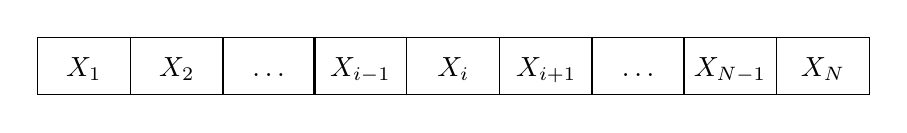
\begin{tikzpicture}[>=latex]
\matrix[mymat,anchor=west,row 1/.style={nodes=draw}]
at (0,0) 
(mat1)
{
X_{1} & X_{2} &  & \ldots &  & X_{i-1} & X_{i} & X_{i+1} & & \ldots &  & X_{N-1} & X_{N} \\
};
\end{tikzpicture}
\caption{\emph{1-D} regionalized variable.}
\label{fig:1DmodelArray}
\end{figure} 


\subsubsection{\texorpdfstring{\emph{1-D}}{1D} Markov Chain}

In the markovian scenario, the probabilistic model exhibits the following spatial dependence: given the present, the future is independent of the past. For the proposed setting, see Fig. \ref{fig:1DmodelArray}, a past-present-future sorting has been imposed from location 1 to the location N.

Let $X_{1}, X_{2}, , \ldots ,  , X_{i-1} , X_{i} , X_{i+1} ,  , \ldots ,  , X_{N-1} , X_{N}$ be a sequence of random variables taking values in a state space ($\mathcal{A} = \left\{ \mathcalligra{a}_{1}, \mathcalligra{a}_{2}, \ldots , \mathcalligra{a}_{ \left| \mathcal{A} \right| } \right\} $). Then, the markovian property states that:


\begin{equation}
\label{eq:Markov_Property}
	 Pr( X_{i} = \mathcalligra{a}_{k} | \  X_{i-1} = \mathcalligra{a}_{l}, X_{i-2} = \mathcalligra{a}_{m}, \ldots , X_{1} = \mathcalligra{a}_{p})  = Pr(X_{i} = \mathcalligra{a}_{k} | \ X_{i-1} = \mathcalligra{a}_{l}) .
\end{equation}


In addition, under the assumption of stationarity and time invariance, the transition probability is given by:

\begin{equation}
\label{eq:Markov_TransProb}
	p_{ l,k } =  Pr(X_{i} = \mathcalligra{a}_{k} | X_{i-1} = \mathcalligra{a}_{l} ) .
\end{equation}

From this transition probability the \emph{1-D} markov chain can be described by its transition matrix:

\begin{equation}
\label{eq:Markov_TransMatrix}
	p = \left|	\begin{array}{cccccc}
			p_{1,1} & p_{1,2} & \ldots & \ & \ldots & p_{1, \left| \mathcal{A} \right| } \\
			p_{2,1} & \ & \ldots & \ & \ldots & \ \\
			\ldots & \ & \ldots & \ & \ldots & \ \\
			\ & \ & \ldots & p_{l, k } & \ldots & \ \\
			\ldots & \ & \ldots & \ & \ldots & \ \\			
			p_{\left| \mathcal{A} \right|,1} & \ & \ldots & \ & \ldots & p_{\left| \mathcal{A} \right|, \left| \mathcal{A} \right| }
	\end{array}  \right|
\end{equation}
with $p_{l,k}$ denoting the probability of transition from $\mathcalligra{a}_{l}$ to $\mathcalligra{a}{k}$,  $ \forall  l,k \in \left\{ 1, \ldots, \left| \mathcal{A} \right| \right\}$. This transition probability is called single step transition because is related with the transition between two consecutive elements of the sequence of random variables, $\left\{X_{i}\right\}$. Extending this idea, the transition probability can be characterized relating elements, in the random sequence, separated by $M$ steps by the multiplication of the single step transition matrix by itself $M$ times. Thus:

\begin{equation}
\label{eq:Markov_TransProbM}
	Pr(X_{i} = \mathcalligra{a}_{k} | X_{i-M} = \mathcalligra{a}_{l}, X_{i-M-1} = \mathcalligra{a}_{m}, \ldots , X_{1} = \mathcalligra{a}_{p} ) =  Pr(X_{i} = \mathcalligra{a}_{k} | X_{i-M} = \mathcalligra{a}_{l} ) = \left(p^{M}\right)_{ l,k } .
\end{equation}


\subsubsection{Joint probability mass of the sequence $\left\{ X_{i} \right\}$}

For a \emph{1-D} markov chain the joint probability mass function can be written as:

\begin{equation}
\label{eq:Markov_PMF}
	p(x_{1},x_{2},\ldots,x_{N}) = p(x_{1}) \cdot \prod_{r=2}^{N}{p(x_{r} | x_{r-1})}
\end{equation}

Then, the Joint Entropy for the sequence $\left\{ X_{i} \right\}$, using the theorem 2.5.1 in \cite{cover_2006}, is described by:

\begin{equation}
\label{eq:Markov_JointH}
	H(X_{1},X_{2}, \ldots , X_{N}) = \sum_{i=1}^{N}{H(X_{i} | X_{i-1}, X_{i-2} \ldots , X_{1})} =  \sum_{i=1}^{N}{H(X_{i} | X_{i-1})}
\end{equation}

The conditional probability can be given from the transition matrix $p$. For the two point joint probability $p(x_{i},x_{i-1})$ , using the fact that $p(x_{i},x_{i-1}) = p(x_{i-1}) \cdot p(x_{i} \ | \ x_{i-1})$. Finally, given the marginal entropy for the initial state $X_{1}$, the remaining marginal can be expressed by:

\begin{equation}
\label{eq:Markov_marginalP}
	p(x_{i}) = \sum_{x_{i-1} \in \mathcal{A}}{ p(x_{i-1}) \cdot p(x_{i} \ |  \ x_{i-1}) }
\end{equation}

\subsubsection{Conditioning to a subset of states}

The main challenge is to apply the proposed \emph{OSP} approach to the \emph{1-D} markov chain. As presented in sec. \ref{sec_adaptive_seq_sensing_PI}, the entropy based \emph{OSP} can be stated in several equivalent ways. First, given a subset of previously measured locations (or at least selected to be measured), the target is to find the non measured location with maximum entropy, $X^{*}_{i} = argmax H(X_{i} \ | \  X_{Measured})$. Alternatively, it can be asked for the location minimizing the posterior entropy for the remaining non measured locations, $X^{*}_{i} = argmin H(X_{NoMeasured \ \setminus \ i} \ | \ X_{Measured, i}) $. These formulations require the joint \emph{pmf}s of the random variables at the unmeasured locations conditioned to the subset of the variables at the measured locations, $p( x_{i} \ | \  x_{Measured})$  or $p( x_{NoMeasured} \ | \  x_{Measured})$,  respectively.

\subsubsection{Conditioning to any arbitrary subset of states}
%To obtain the entropy of a state $X_{i}$, conditioned by the subset of measured locations $X_{Measured}$. The subset can be split in two disjoint subsets denoting the past and the futures variables, $\left\{XB\right\}$ and $\left\{XA\right\}$ respectively, conditioning the state $X_{i}$:

Let $\left\{X_{b_{j}}\right\}$ and $\left\{X_{a_{j}}\right\}$ be two disjoint subsets denoting the past and the futures variables conditioning the state $X_{i}$. Then the measured locations can be represented by $X_{Measured}  =  \left\{X_{b_{j}}\right\} \bigcup \left\{X_{a_{j}}\right\}$, as illustrated in Fig. \ref{fig:1DmodelArray_BA_Subsets}.



\begin{figure}[H]
		\centering
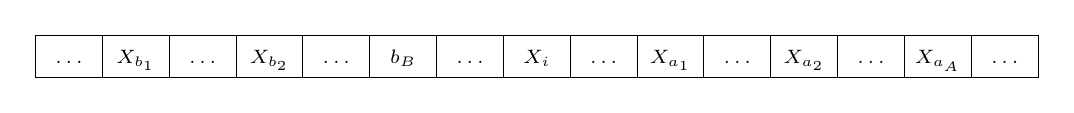
\begin{tikzpicture}[>=latex]
\scriptsize
\matrix[mymat,anchor=west,row 1/.style={nodes=draw}]
at (0,0) 
(mat1)
{
\ldots & X_{b_{1}} & \ldots & X_{b_{2}} & \ldots & b_{B} & \ldots & X_{i} & \ldots & X_{a_{1}} & \ldots & X_{a_{2}} & \ldots & X_{a_{A}} & \ldots \\
};
\end{tikzpicture}
\caption{Measured Variables in separated past and future subsets.}
\label{fig:1DmodelArray_BA_Subsets}
\end{figure} 

Then, the target conditional entropy for the state $X_{i}$, can be defined as:
                   
\begin{align}
\label{eq:Markov_CondAB_H}
	H(X_{i} \ | \ \left\{X_{b_{j}}\right\} & , \left\{X_{a_{j}}\right\}) \nonumber \\
	&= - \sum_{  \left\{x_{b_{j}}\right\} \in \mathcal{A}^{B}  }{ \ \ \sum_{ x_{i} \in \mathcal{A} }{ \ \ \sum_{  \left\{x_{a_{j}}\right\} \in \mathcal{A}^{A}      }{ p(\left\{x_{b_{j}}\right\} , x_{i}, \left\{x_{a_{j}}\right\}) \cdot log \ p(x_{i} \ | \ \left\{x_{b_{j}}\right\} , \left\{x_{a_{j}}\right\})   }}}
\end{align}

Furthermore, it is possible to rewrite 
\eqref{eq:Markov_CondAB_H} by using the definition of the conditional entropy as the expected value of the entropies of the conditional distributions, averaged over the conditioning random variables [Chapter 2.2, \cite{cover_2006}].


\begin{align}
\label{eq:Markov_CondAB_H_MargCond}
	H(X_{i} &  \ | \ \left\{X_{b_{j}}\right\} , \left\{X_{a_{j}}\right\})  \nonumber \\
	& = \sum_{  \left\{x_{b_{j}}\right\} \in \mathcal{A}^{B}  }{}{ \ \ \sum_{  \left\{x_{a_{j}}\right\} \in \mathcal{A}^{A}      }{ p(\left\{x_{b_{j}}\right\} , \left\{x_{a_{j}}\right\}) \cdot H(X_{i} \  | \ \left\{X_{b_{j}}\right\} = \left\{x_{b_{j}}\right\} , \left\{X_{a_{j}}\right\} = \left\{x_{a_{j}}\right\})   }}
\end{align}



In one hand, to evaluate the expression from \eqref{eq:Markov_CondAB_H}, it is required to work in the conditional \emph{pmf} of the state $X_{i}$. Thus, using the relationship of the joint \emph{pmf} and the conditional \emph{pmf}:


\begin{align}\label{eq:Markov_CondAB_pmf}
 p(x_{i} \ | \ \left\{x_{b_{j}}\right\} , \left\{x_{a_{j}}\right\}) & = \frac{p(\left\{x_{b_{j}}\right\} , x_{i}, \left\{x_{a_{j}}\right\})}{p(\left\{x_{b_{j}}\right\} , \left\{x_{a_{j}}\right\})} \nonumber \\
    & = \frac{p(\left\{x_{b_{j}}\right\} , x_{i}, x_{a_{1}}, x_{a_{2}}, \ldots,  x_{a_{A}})}{p(\left\{x_{b_{j}}\right\} , x_{a_{1}}, x_{a_{2}}, \ldots,  x_{a_{A}})} \nonumber \\
		    & = \frac{p(x_{a_{A}} \ | \ \left\{x_{b_{j}}\right\} , x_{i}, x_{a_{1}}, x_{a_{2}}, \ldots,  x_{a_{A-1}}) \cdot p(\left\{x_{b_{j}}\right\} , x_{i}, x_{a_{1}}, x_{a_{2}}, \ldots,  x_{a_{A-1}})}{ p(x_{a_{A}} \ | \   \left\{x_{b_{j}}\right\} , x_{a_{1}}, x_{a_{2}}, \ldots,  x_{a_{A-1}})  \cdot p(\left\{x_{b_{j}}\right\} , x_{a_{1}}, x_{a_{2}}, \ldots,  x_{a_{A-1}})} \nonumber \\
				\text{\tiny{by markovian property}}  & = \frac{p(x_{a_{A}} \ | \  x_{a_{A-1}}) \cdot p(\left\{x_{b_{j}}\right\} , x_{i}, x_{a_{1}}, x_{a_{2}}, \ldots,  x_{a_{A-1}})}{ p(x_{a_{A}} \ | \  x_{a_{A-1}})  \cdot p(\left\{x_{b_{j}}\right\} , x_{a_{1}}, x_{a_{2}}, \ldots,  x_{a_{A-1}})} \nonumber \\
				  & = \frac{ p(\left\{x_{b_{j}}\right\} , x_{i}, x_{a_{1}}, x_{a_{2}}, \ldots,  x_{a_{A-1}})}{ p(\left\{x_{b_{j}}\right\} , x_{a_{1}}, x_{a_{2}}, \ldots,  x_{a_{A-1}})} \nonumber \\
\end{align}

From Eq. \eqref{eq:Markov_CondAB_pmf}, the effect of the most future state, $X_{a_{A}}$,  vanishes for the markovian property and the presence of the closer future state, $X_{a_{A-1}}$. Furthermore, iterating the same principle for the rest of the variables in the subset of future states, it can post that:


\begin{align}\label{eq:Markov_CondAB_pmf_2}
 p(x_{i} \ | \ \left\{x_{b_{j}}\right\} , \left\{x_{a_{j}}\right\}) & = \frac{ p(\left\{x_{b_{j}}\right\} , x_{i}, x_{a_{1}})}{ p(\left\{x_{b_{j}}\right\} , x_{a_{1}})} \nonumber \\
            & = p(x_{i} \ | \ \left\{x_{b_{j}}\right\} , x_{a_{1}}) \nonumber \\
\end{align}


From the above result, for a markovian chain, given a subset of future states, ${x_{a_{j}}}$, conditioning the present state, $X_{i}$, then the present state depends only the nearest future state that is part of the subset. The essence of this result was presented by \cite{Elfeki2001_a} by the formulation of the conditional probability $p(x_{i} \ | \ x_{i-1} ,x_{N} )$.

In Eq. \eqref{eq:Markov_CondAB_pmf_2}, it is required to reduce the dependence related with the subset of past states. Thus,


\begin{align}\label{eq:Markov_CondAB_pmf_3}
 p(x_{i} \ | \ \left\{x_{b_{j}}\right\} , \left\{x_{a_{j}}\right\}) & = \frac{ p(\left\{x_{b_{j}}\right\} , x_{i}, x_{a_{1}})}{ p(\left\{x_{b_{j}}\right\} , x_{a_{1}})} \nonumber \\
                 & = \frac{  p(x_{a_{1}}  \ | \ \left\{x_{b_{j}}\right\} ,   x_{i} ) \cdot p(\left\{x_{b_{j}}\right\} ,   x_{i} )   }{      p(x_{a_{1}} \ | \ \left\{x_{b_{j}}\right\} ) \cdot p(\left\{x_{b_{j}}\right\}  ) } \nonumber \\
				\text{\tiny{by markovian property}}  & = \frac{  p(x_{a_{1}}  \ | \   x_{i} ) \cdot p(\left\{x_{b_{j}}\right\} ,   x_{i} )   }{      p(x_{a_{1}} \ | \ \left\{x_{b_{j}}\right\} ) \cdot p(\left\{x_{b_{j}}\right\}  ) } \nonumber \\
				  & = \frac{  p(x_{a_{1}}  \ | \   x_{i} ) \cdot p(x_{i}  \ | \ \left\{x_{b_{j}}\right\}) \cdot p(\left\{x_{b_{j}}\right\} )   }{      p(x_{a_{1}} \ | \ \left\{x_{b_{j}}\right\} ) \cdot p(\left\{x_{b_{j}}\right\}  ) } \nonumber \\
\end{align}

Then, simplifying and applying the markovian property Eq. \eqref{eq:Markov_CondAB_pmf_3} can be reduced to:


\begin{align}\label{eq:Markov_CondAB_pmf_4}
 p(x_{i} \ | \ \left\{x_{b_{j}}\right\} , \left\{x_{a_{j}}\right\}) & = \frac{  p(x_{a_{1}}  \ | \   x_{i} ) \cdot p(x_{i}  \ | \ \left\{ x_{b_{j}}\right\})  }{      p(x_{a_{1}} \ | \ \left\{x_{b_{j}}\right\} )  }  \nonumber \\
				\text{\tiny{by markovian property}}  & =  \frac{  p(x_{a_{1}}  \ | \   x_{i} ) \cdot p(x_{i}  \ | \ x_{b_{B}})  }{      p(x_{a_{1}} \ | \ x_{b_{B}} )  }  \nonumber \\
\end{align}

In other words,

\begin{equation}
\label{eq:Markov_CondAB_pmf_5}
p(x_{i} \ | \ \left\{x_{b_{j}}\right\} , \left\{x_{a_{j}}\right\}) = p(x_{i} \ | \ x_{b_{B}} , x_{a_{1}})
\end{equation}


Summarizing the last results, conditioning a state $X_{i}$ by any subset of states reduce to conditional bivariate \emph{pmf}s only relating $X_{i}$ to the nearest past and to the nearest future states inside the set of measured variables.

In the other hand, to calculate the required conditional entropy, the joint \emph{pmf} is needed, $p(\left\{x_{b_{j}}\right\} , x_{i}, \left\{x_{a_{j}}\right\})$. Applying Eq. \eqref{eq:Markov_PMF}:

\begin{align}
\label{eq:Markov_JointAB_pmf}
p(\left\{x_{b_{j}}\right\} & , x_{i}, \left\{x_{a_{j}}\right\})   \nonumber \\
& = p(x_{b_{1}}) \cdot \left[ \prod_{h = 2}^{B}{p(x_{b_{h}} \ | \ x_{b_{h-1}})} \right] \cdot p(x_{i} \ | \ x_{b_{B}}) \cdot p(x_{a_{1}} \ | \ x_{i}) \cdot \left[ \prod_{h = 2}^{A}{p(x_{a_{h}} \ | \ x_{a_{h-1}})}  \right]
\end{align}

In short, Eq. \eqref{eq:Markov_CondAB_pmf_4} and Eq. \eqref{eq:Markov_JointAB_pmf} can be expressed in terms of marginal and two points conditional probabilities. At this point, all the information required to efficiently calculate Eq. \eqref{eq:Markov_CondAB_H} is available, and consequently it is possible to solve the \emph{MES} rule. All conditional probabilities, in Eq. \eqref{eq:Markov_CondAB_pmf_4} and Eq. \eqref{eq:Markov_JointAB_pmf}, can be estimated from the transition matrix by the n-step transition probabilities from Eq. \eqref{eq:Markov_TransProbM}. In addition, the marginal probabilities for $p(x_{b_{1}})$ required in Eq. \eqref{eq:Markov_JointAB_pmf}, can be iteratively calculated \citep{cover_2006} by:

\begin{equation}
\label{eq:Markov_Marginal_pmf}
	p(x_{i}) = \sum_{x_{i-1} \in \mathcal{A}}{ p(x_{i-1}) \cdot p(x_{i} | x_{i-1})}
\end{equation}

In brief, as expected for a \emph{1-D} Markov chain, all the conditional entropy characterization relies on the transition matrix and the initial marginal distribution for the state $X_{1}$.

In addition, using Eq. \eqref{eq:Markov_CondAB_pmf_5} the target entropy of the conditional distribution for the state $X_{i}$, can be defined as:
                   
\begin{align}
\label{eq:Markov_CondAB_H_Reduced}
	H(X_{i} \ | \ \left\{X_{b_{j}}\right\} = \left\{x_{b_{j}}\right\} & , \left\{X_{a_{j}}\right\} = \left\{x_{a_{j}}\right\}) \nonumber \\
	& = - \sum_{ x_{i} \in \mathcal{A} }{ p(x_{i} \ | \ \left\{x_{b_{j}}\right\} , \left\{x_{a_{j}}\right\}) \cdot log \ p(x_{i} \ | \ \left\{x_{b_{j}}\right\} , \left\{x_{a_{j}}\right\})   }   \nonumber \\
	    \text{\tiny{by Eq. \eqref{eq:Markov_CondAB_pmf_5}}}  & =  - \sum_{ x_{i} \in \mathcal{A} }{ p(x_{i} \ | \ x_{b_{B}} , x_{a_{1}}) \cdot log \ p(x_{i} \ | \ x_{b_{B}} , x_{a_{1}})   }   \nonumber \\
			 & =  H(X_{i} \ | \ X_{b_{B}} = x_{b_{B}} , X_{a_{1}} = x_{a_{1}})
\end{align}

Then, from Eq. \eqref{eq:Markov_CondAB_H_MargCond} and Eq. \eqref{eq:Markov_CondAB_H_Reduced}, the conditional entropy can be formulated as:

\begin{equation}
\label{eq:Markov_CondAB_H_Reduced_WithMargCond}
	H(X_{i} \ | \ \left\{X_{b_{j}}\right\} , \left\{X_{a_{j}}\right\}) = \sum_{  \left\{x_{b_{j}}\right\} \in \mathcal{A}^{B}  }{ }{ \ \ \sum_{  \left\{x_{a_{j}}\right\} \in \mathcal{A}^{A}      }{ p(\left\{x_{b_{j}}\right\} , \left\{x_{a_{j}}\right\}) \cdot H( X_{i} \ | \ X_{b_{B}} = x_{b_{B}} , X_{a_{1}} = x_{a_{1}})   }}
\end{equation}

A preliminary attempt to reduce the Eq. \eqref{eq:Markov_CondAB_H_Reduced_WithMargCond} consisted in properly separating the conditional variables:

%\tiny

\begin{align}
\label{eq:Markov_CondAB_H_reducing}
	H(X_{i} \ | & \ \left\{X_{b_{j}}\right\} , \left\{X_{a_{j}}\right\})  \nonumber \\
	= & \sum_{  \left\{x_{b_{j}}\right\} \setminus x_{b_{B}} \in \mathcal{A}^{B-1}  }\sum_{  x_{b_{B}} \in \mathcal{A}} \ \ \sum_{  \left\{x_{a_{j}}\right\} \setminus x_{a_{1}} \in \mathcal{A}^{A-1} }\sum_{x_{a_{1}} \in \mathcal{A} } \left[ \right. \nonumber \\
	& \ \ \ \ \ \ \ \ \ \ \ \ p(\left\{x_{b_{j}}\right\} \setminus x_{b_{B}}, x_{b_{B}} , \left\{x_{a_{j}}\right\} \setminus x_{a_{1}}, x_{a_{1}}) \cdot H( X_{i} \ | \ X_{b_{B}} = x_{b_{B}} , X_{a_{1}} = x_{a_{1}})   \left. \right]   \nonumber \\
	\nonumber \\
	\text{\tiny{By Bayes}} = & \sum_{  \left\{x_{b_{j}}\right\} \setminus x_{b_{B}} \in \mathcal{A}^{B-1}  }\sum_{  x_{b_{B}} \in \mathcal{A}} \sum_{  \left\{x_{a_{j}}\right\} \setminus x_{a_{1}} \in \mathcal{A}^{A-1} }\sum_{x_{a_{1}} \in \mathcal{A} } \left[ \right. \nonumber \\
	& \ \ \ \  p(x_{b_{B}} , x_{a_{1}} \ | \ \left\{x_{b_{j}}\right\} \setminus x_{b_{B}} , \left\{x_{a_{j}}\right\} \setminus x_{a_{1}}) \cdot p(x_{b_{B}} , x_{a_{1}})  \cdot H( X_{i} \ | \ X_{b_{B}} = x_{b_{B}} , X_{a_{1}} = x_{a_{1}})     \left. \right]  \nonumber \\
	\nonumber \\
	= & H( X_{i} \ | \ X_{b_{B}}, X_{a_{1}} ) \cdot \sum_{  \left\{x_{b_{j}}\right\} \setminus x_{b_{B}} \in \mathcal{A}^{B-1}  }\sum_{  x_{b_{B}} \in \mathcal{A}} \sum_{  \left\{x_{a_{j}}\right\} \setminus x_{a_{1}} \in \mathcal{A}^{A-1} }\sum_{x_{a_{1}} \in \mathcal{A} } \left[ \right. \nonumber \\
	&  \ \ \ \ \ \ \ \ \ p(x_{b_{B}} , x_{a_{1}} \ | \ \left\{x_{b_{j}}\right\} \setminus x_{b_{B}} , \left\{x_{a_{j}}\right\} \setminus x_{a_{1}})  \left. \right]   \nonumber \\	
		= & H( X_{i} \ | \ X_{b_{B}}, X_{a_{1}} ) 
\end{align}
\normalsize

Only for these two conditioning variables:

\begin{align}
\label{eq:Markov_CondAB_H_Reduced_FullNom_FORTWO}
	H(X_{i} \ | \ X_{b_{B}} , X_{a_{1}}) = & - \sum_{  x_{b_{B}} \in \mathcal{A}  }{ \ \ \sum_{ x_{i} \in \mathcal{A} }{ \ \ \sum_{  x_{a_{1}} \in \mathcal{A}      }{ }}} \left[ \left(   \right. \right.  \nonumber \\
			&	p(X_{b_{B}} = x_{b_{B}}) \cdot p(X_{i} = x_{i} \ | \ X_{b_{B}} = x_{b_{B}}) \cdot p(X_{a_{1}} = x_{a_{1}} \ | \ X_{i} = x_{i})     \nonumber \\
  		& \left. \left.	\right) \cdot log \ p(X_{i} = x_{i} \ | \ X_{b_{B}} = x_{b_{B}} , X_{a_{1}} = x_{a_{1}})  \right]  
\end{align}


Finally, using Eq. \eqref{eq:Markov_CondAB_pmf_4}:

\begin{align}
\label{eq:Markov_CondAB_H_Reduced_FullNom_FORTWO_2}
	H(X_{i} \ | \ X_{b_{B}} , X_{a_{1}}) = & - \sum_{  x_{b_{B}} \in \mathcal{A}  }{ \ \ \sum_{ x_{i} \in \mathcal{A} }{ \ \ \sum_{  x_{a_{1}} \in \mathcal{A}      }{ }}} \left[ \left(   \right. \right.  \nonumber \\
			&	p(X_{b_{B}} = x_{b_{B}}) \cdot p(X_{i} = x_{i} \ | \ X_{b_{B}} = x_{b_{B}}) \cdot p(X_{a_{1}} = x_{a_{1}} \ | \ X_{i} = x_{i})     \nonumber \\
  		& \left. \left.	\right) \cdot log  \  \left(      \frac{  p(x_{a_{1}}  \ | \   x_{i} ) \cdot p(x_{i}  \ | \ x_{b_{B}})  }{      p(x_{a_{1}} \ | \ x_{b_{B}} )  }   \right)     \right]  
\end{align}






































































\newpage
\section{Formulation and Implementation of Noisy Sparse Promoting Solvers}
\label{sec_Meth_aNSR}

Given sampling schemes provided by \emph{OSP}, its comparison with some sparse promoting oriented schemes has been proposed by the modification of classical $L1$ minimizers solver (available in the $L1$ magic and \emph{CVX} software). The contribution has been focused on formulating the signal recovery process as a generalized sampling problem. The idea relies on to take advantage of the sparse nature of channelized structures, the reduced spatial variations of the \emph{2-D} images in the proposed database and the use of a prior statistical model as an additional source of information related with spatial dependencies and pixel uncertainty.  

Therefore, applying principles from \emph{Noisy compressive Sensing} (\emph{NCS}) to the reconstruction of binary channels of permeability for the estimation of the model, it is possible to use \emph{MPS} realizations as a source of statistical data. In particular, it allows the estimation of variance and covariance of the target regionalized variables.

\subsection{\emph{NCS} and \textit{Whitening} process}

The main idea supporting this preliminary work was to consider the noise associated to measurements in the sparse recovery solver. 

The noise associated to measurements has been incorporated in the sparse recovery solver relaxing the search space. In this way, given a small amount of noisy measurements from geologic data ($m$ measures from a field of $N$ variables, with $m << N$), the target is to reconstruct the \emph{actual} channel. While traditional \emph{CS} approaches deal with time-invariant sparse signals without error in measurements, the motivation was supported by the next hypothesis: 1) \emph{NCS} provides a theory of signal recovery from highly incomplete noisy information, and 2) \emph{MPS} could provide information about signal variability required to the noise characterization on \emph{NCS} framework.

Thus, a preliminary framework of \emph{NCS} has been  implemented and validated oriented to improve \emph{MPS} performance. Standard \emph{CS} implementation for channelized binary structures was proposed and implemented for others members of the \emph{IDS} Lab \footnote{Information and Decision Systems Laboratory, \emph{IDS} Lab, at Electrical Engineering Department, Universidad de Chile.}. The reader is referred to \cite{Calderon2015_a} for more details on this approximation. Classical conditions and theory of \emph{NCS} was described in sections \ref{subSecBasicCSFor} and \ref{subSecGeneralNCS}.

%In an initial stage
Here, previous works are extended in order to consider noisy measures, providing a framework to noise characterization. In order to apply the theory of \emph{NCS} a signal model with white noise is required, then a whitening process is needed to use the proposed methods. Thus,the next \emph{sensing model} has been considered: \\

\begin{align}
	 I & = \Phi \cdot Z     \\ 
	 X & = I(:)             \\
	 Y_{Sampled} & = A \cdot X + \xi 
\label{eq_NCS_Model_UsModel}
\end{align}


{with}

			\begin{itemize}
					\item $Z$    ($M$ x $M$)   : Signal in transformed domain (in this case a \emph{2-D} \emph{DCT} coefficients matrix of size $200$ x $200$)
					\item $\Phi$ ($M$ x $M$)   : Transform matrix (inverse \emph{DCT} in this work)

					\item $I$    ($M$ x $M$)   : Image in canonical domain
					\item $X$    ($N$ x $N$)   : Vectorization of signal in image domain ($N$ = $M$ x $M$, in this case $40000$)
					
					\item $A$    ($m$ x $N$) : Sampling matrix (m vectors randomly taken from $N$ x $N$ Identity matrix) 										
															
					\item $Y_{Sampled}$    ($m$ x $1$)   : vector of $m$ measurements (including Hard and Soft Data) 
					\item $\xi$  ($m$ x $1$)   : vector of noise in measurements, with covariance matrix $C_v$ and mean $\xi_{mean}$.
			\end{itemize}
	
At this point the Eq. \eqref{eq_NCS_Model_UsModel} only differs from \cite{Calderon2015_a} approach in the incorporation of noise component. Here, the noise $\xi$ would be a spatially correlated noise, requiring a \emph{whitening} pre-processing.

	
A signal model with zero mean noise has been described by the subtraction of the mean of noise $\xi_{mean}$ obtaining: \\
	
	\begin{align}
			Y_{Sampled} - \xi_{mean} = A \cdot X + \xi - \xi_{mean}
			\label{eq_NCS_Model_UsModel_zeroMean_Full}
\end{align}

Defining zero mean variables and rewriting the expression in Eq. \eqref{eq_NCS_Model_UsModel_zeroMean} is: \\

\begin{align}
			Y_{0} = A \cdot X + \xi_{0}
			\label{eq_NCS_Model_UsModel_zeroMean}
\end{align}
					
From Eq. \eqref{eq_NCS_Model_UsModel_zeroMean} it is required an additional process to obtain a model with a non correlated noise. In order to achieve a sensing model under white noise and assuming the existence of an invertible covariance matrix for $\xi_{0}$ the next formulation has been achieved: \\

	\begin{align}
			C_{v}^{\frac{-1}{2}} \cdot Y_{0} & = C_{v}^{\frac{-1}{2}} \cdot A \cdot X + C_{v}^{\frac{-1}{2}} \cdot \xi_{0} \\
			C_{v}^{\frac{-1}{2}} \cdot Y_{0} & = C_{v}^{\frac{-1}{2}} \cdot A \cdot X + \eta  \\
			\widehat{Y} & = C_{v}^{\frac{-1}{2}} \cdot A \cdot X + \eta	
			\label{eq_NCS_Model_UsModel_whitenoise_Generic}
\end{align}						

Finally, replacing the vectorization process:

	\begin{align}
			\widehat{Y} & = C_{v}^{\frac{-1}{2}} \cdot A \cdot VEC(\Phi \cdot Z) + \eta 	
			\label{eq_NCS_Model_UsModel_whitenoise}
\end{align}						

	
The Eq. \eqref{eq_NCS_Model_UsModel_whitenoise} fits the classical framework of \emph{NCS} for signals under white noise model. The selection of the sampling matrix $A$ satisfies isotropic property, the vectorization process $VEC(\cdot)$ retain spatial dependence in the regionalized field, the basis DCT provides a domain where the signal is compressible, and $C_{v}$ is estimated as the experimental covariance of realizations of \emph{MPS}.






























%\section{Incorporation of Virtual Noisy Measures by \emph{MPS}}
%\label{sec_Meth_iVNM}


%\section{Integration of \emph{OWP} and \emph{NCS}}
%\label{sec_Meth_iOWPandNCS}

%\subsection{Bayesian Methods}

%MAP estmn. using a sparse linear model
%Also a regression problem with sparsity
%promoting penalties (e.g., lp-norm)
%l1-min (BP/LASSO) is a special case

%MAP Estimation
%\begin{align}
%	\[ \mathbf{x}^{*} = argmax_{\mathbf{x}}{p\left( \mathbf{x} | \mathbf{y}   \right) } \]
%	\[ \mathbf{x}^{*} = argmin_{\mathbf{x}}{- log \left( p\left( \mathbf{y} | \mathbf{x}\right) \right) - log \left( p \left( \mathbf{x} \right) \right) } \]	
%	\[ \mathbf{x}^{*} = argmin_{\mathbf{x}}{ \left\| \mathbf{y} - \Phi \cdot \mathbf{x} \right\|_{2}^{2}  + \lambda \cdot \sum_{i = 1}^{N}{g \left( \left| x_{i} \right| \right) }} \]	
%\end{align}

%where $g \left( \left| x_{i} \right| \right)$ represents a Separable Prior.

%For sparse solutions, g(|xi|) should be a concave,
%nondecreasing function
%Example: $g \left( \left| x_{i} \right| \right) = \left| x_{i} \right|^{p}$ with $p \leq 1$
%Lasso is a special case: $p = 1$
%Any local min. of the MAP estmn problem has at
%most M nonzeros (Rao et al., 99)







\subsection{On Noisy Compressive Sensing Performance}
\label{sec_exp_NCS_APP}


\emph{NCS} theory has been a motivation to study the spatial co-dependencies of the regionalized variable of interest. heretofore, how \emph{MPS} can help in achieving this task have been investigated and it generated a preliminary analysis of how the incorporation of spatial dependence improves sparse promoting algorithms.

\subsubsection{Statistical Analysis from \emph{MPS}}

Using the data base of multichannel \emph{$MC_{1}$} model, obtained $200$ \emph{MPS} realizations has been obtained from several sampling rates. For each sampling regime, the second order statistics has been estimated. As shown in fig. \ref{fig:StatsMC1} the field variance in low rate sampling regimes is higher than in regimes with more measurements. In the extreme case of $0.1 \% $ measurements, the variance at most field positions was extremely uncertain. As the measurements increased a reduction of non local variance has been observed, thereby the powerful of spatial conditioning from \emph{MPS} has been validated.

		\begin{figure}[H]
		\centering
		\centerline
		{
			\begin{subfigure}[b]{0.15\textwidth}
				\includegraphics[width=\textwidth]{Figs_Slides/01_Orig.png}
			\end{subfigure}
			\begin{subfigure}[b]{0.15\textwidth}
					\includegraphics[width=\textwidth]{Figs_Slides/05_Orig.png}
			\end{subfigure}
			\begin{subfigure}[b]{0.15\textwidth}
					\includegraphics[width=\textwidth]{Figs_Slides/1_Orig.png}
			\end{subfigure}
			\begin{subfigure}[b]{0.15\textwidth}
					\includegraphics[width=\textwidth]{Figs_Slides/2_Orig.png}
			\end{subfigure}
			\begin{subfigure}[b]{0.15\textwidth}
					\includegraphics[width=\textwidth]{Figs_Slides/3_Orig.png}
			\end{subfigure}
			\begin{subfigure}[b]{0.15\textwidth}
					\includegraphics[width=\textwidth]{Figs_Slides/4_Orig.png}
			\end{subfigure}
			\begin{subfigure}[b]{0.15\textwidth}
					\includegraphics[width=\textwidth]{Figs_Slides/5_Orig.png}
			\end{subfigure}
		}
		\centerline{
			\begin{subfigure}[b]{0.15\textwidth}{\includegraphics[width=\textwidth]{Figs_Slides/01_Mean.png}}
			\end{subfigure}
			\begin{subfigure}[b]{0.15\textwidth}{\includegraphics[width=\textwidth]{Figs_Slides/05_Mean.png}}
			\end{subfigure}
			\begin{subfigure}[b]{0.15\textwidth}{\includegraphics[width=\textwidth]{Figs_Slides/1_Mean.png}}
			\end{subfigure}
			\begin{subfigure}[b]{0.15\textwidth}{\includegraphics[width=\textwidth]{Figs_Slides/2_Mean.png}}
			\end{subfigure}
			\begin{subfigure}[b]{0.15\textwidth}{\includegraphics[width=\textwidth]{Figs_Slides/3_Mean.png}}
			\end{subfigure}
			\begin{subfigure}[b]{0.15\textwidth}{\includegraphics[width=\textwidth]{Figs_Slides/4_Mean.png}}
			\end{subfigure}
			\begin{subfigure}[b]{0.15\textwidth}{\includegraphics[width=\textwidth]{Figs_Slides/5_Mean.png}}
			\end{subfigure}
		}
		\centerline{		
			\begin{subfigure}[b]{0.15\textwidth}{\includegraphics[width=\textwidth]{Figs_Slides/01_Std.png}}
			\end{subfigure}
			\begin{subfigure}[b]{0.15\textwidth}{\includegraphics[width=\textwidth]{Figs_Slides/05_Std.png}}
			\end{subfigure}
			\begin{subfigure}[b]{0.15\textwidth}{\includegraphics[width=\textwidth]{Figs_Slides/1_Std.png}}
			\end{subfigure}
			\begin{subfigure}[b]{0.15\textwidth}{\includegraphics[width=\textwidth]{Figs_Slides/2_Std.png}}
			\end{subfigure}
			\begin{subfigure}[b]{0.15\textwidth}{\includegraphics[width=\textwidth]{Figs_Slides/3_Std.png}}
			\end{subfigure}
			\begin{subfigure}[b]{0.15\textwidth}{\includegraphics[width=\textwidth]{Figs_Slides/4_Std.png}}
			\end{subfigure}
			\begin{subfigure}[b]{0.15\textwidth}{\includegraphics[width=\textwidth]{Figs_Slides/5_Std.png}}
			\end{subfigure}
		}
		
			\caption{Statistics from simulations.}
			\scriptsize{ For scenarios considering 0.1 \%, 0.5 \%, 1 \%, 2 \%, 3 \%, 4 \%, and 5 \% of hard data measures.}
		\label{fig:StatsMC1}	
\end{figure}		

As expected for \emph{MPS}, these preliminary outcomes shown that statistical analysis from \emph{MPS} realizations provides some kind of information about the variability of the value of a non measured pixel from the knowledge of positions and values of hard data measurements. This validate the use of \emph{MPS} realizations as an estimation of the spatial covariance between regionalized variables conforming the stochastic field.

In next subsections several attempts of incorporating information from \emph{MPS} realizations in the \emph{NCS} problem has been explored. The main idea was to provide an estimation of covariance matrix and to use it in whitening process.


\subsubsection{\emph{NCS}. Naive Approach I. what Covariance?}

The most simple assumption was considered that there was no correlation between regionalized variables, and that all variables was modeled incorporating only withe noise with zero mean and the same variance for all the regionalized variables. Under this assumption the variance noise at each individual variable was estimated directly by pixel variance estimation from \emph{MPS} realizations.

At standard \emph{CS} approaches only measurements are considered as input to the reconstruction methods and no one knowledge is given for unmeasured regionalized variables. The incorporation of \emph{MPS} allows no only statistical analysis for global stochastic field, but also the opportunity of considering simulated regionalized variables as noisy virtual measures. 

Here most naive \emph{NCS} approach correspond to consider the model from Eq. \eqref{eq_NCS_Model_UsModel_whitenoise} but with $C_{v}^{\frac{-1}{2}}$ equal to the identity matrix of proper size. Thus, using a mixture of hard data measures and simulated \emph{virtual} measures in standard \emph{CS} does not take advantage of the statistical information provided for the proposed \emph{MPS} analysis because all measurements are considered without uncertainty. The above entails that the \emph{CS} reconstruction would be more close to the specific \emph{MPS} realization than to the real target image. 

		\begin{figure}[H]
		\centering
		\includegraphics[width=0.32	\textwidth]{Figs_Slides/pXY1SNR_NCS.png}
		\includegraphics[width=0.32	\textwidth]{Figs_Slides/pXY2SNR_NCS.png}
		\includegraphics[width=0.32	\textwidth]{Figs_Slides/pXY3SNR_NCS.png}

		\includegraphics[width=0.32	\textwidth]{Figs_Slides/pXY1SSIM_NCS.png}
		\includegraphics[width=0.32	\textwidth]{Figs_Slides/pXY2SSIM_NCS.png}
		\includegraphics[width=0.32	\textwidth]{Figs_Slides/pXY3SSIM_NCS.png}

		\caption[Performance Analysis of Naive Approach of \emph{NCS} by relaxing restrictions]{Performance Analysis of Naive Approach of \emph{NCS} by only relaxing restrictions on soft data.} \scriptsize{ From an initial amount of hard data measurements some level of soft virtual measurements are added from simulations and then \emph{CS} and naive \emph{NCS} approaches are applied. Upper row \emph{SNR} analysis, lower row \emph{SSIM} analysis.From left to right  : initial $1 \%$ of hard data , initial $2 \%$ of hard data, and initial $3 \%$ of hard data.}
		\label{fig:Naive0MC1_Performance}
		\end{figure}
		
As shown in fig. \ref{fig:Naive0MC1_Performance}, partial results on the most naive \emph{NCS} approach present a lower performance than classical \emph{CS}. As reference the performance of \emph{MPS} is shown by the statistics of simulations (mean and variance), \emph{CS} curves consider hard data and soft data as fixed measures while \emph{NCS} allows some uncertainty for these measures. For \emph{SSIM} indicator all reconstructions curves has very close performance, while for \emph{SNR} indicator the classical \emph{CS} achieves a better global performance.  

Without incorporating  spatial correlations on the regionalized variables no advantage from \emph{NCS} theory has been achieved. Including uncertainty on measures only increase the searching space for the optimization algorithms. Thus, the next motivation was to include additional constraints promoting desired features on the regionalized variables. 

The next step has corresponded to incorporate proposed amendments from section \ref{subSecGeneralNCS}. Using alternate recovery models promoting sparsity on signal gradients instead on the signal itself. 

In figure \ref{fig:Naive1MC1}, several configurations of hard and virtual data are presented but considering reconstruction approaches using total variation. In terms of visual inspection is possible to appreciate an improvement in the performance of \emph{NCS}. This behavior is confirmed by analysis of the metrics \emph{SNR} and \emph{SSIM} as shown in fig. \ref{fig:Naive1MC1_Performance}. 

		\begin{figure}
		\centering
		
		\includegraphics[width=0.19	\textwidth]{Figs_Slides/Olds_imTrue.png}
		\includegraphics[width=0.19	\textwidth]{Figs_Slides/Olds_1_1_imNew.png}
		\includegraphics[width=0.19	\textwidth]{Figs_Slides/Olds_1_1_imH8.png}
		\includegraphics[width=0.19	\textwidth]{Figs_Slides/Olds_1_1_imF_DS8.png}
		\includegraphics[width=0.19	\textwidth]{Figs_Slides/Olds_1_1_imF_TV8.png}
		
		\includegraphics[width=0.19	\textwidth]{Figs_Slides/Olds_imTrue.png}
		\includegraphics[width=0.19	\textwidth]{Figs_Slides/Olds_1_10_imNew.png}
		\includegraphics[width=0.19	\textwidth]{Figs_Slides/Olds_1_10_imH8.png}
		\includegraphics[width=0.19	\textwidth]{Figs_Slides/Olds_1_10_imF_DS8.png}
		\includegraphics[width=0.19	\textwidth]{Figs_Slides/Olds_1_10_imF_TV8.png}
		
		\includegraphics[width=0.19	\textwidth]{Figs_Slides/Olds_imTrue.png}
		\includegraphics[width=0.19	\textwidth]{Figs_Slides/Olds_2_7_imNew.png}
		\includegraphics[width=0.19	\textwidth]{Figs_Slides/Olds_2_7_imH8.png}
		\includegraphics[width=0.19	\textwidth]{Figs_Slides/Olds_2_7_imF_DS8.png}
		\includegraphics[width=0.19	\textwidth]{Figs_Slides/Olds_2_7_imF_TV8.png}
				
		\includegraphics[width=0.19	\textwidth]{Figs_Slides/Olds_imTrue.png}
		\includegraphics[width=0.19	\textwidth]{Figs_Slides/Olds_4_4_imNew.png}
		\includegraphics[width=0.19	\textwidth]{Figs_Slides/Olds_4_4_imH8.png}
		\includegraphics[width=0.19	\textwidth]{Figs_Slides/Olds_4_4_imF_DS8.png}
		\includegraphics[width=0.19	\textwidth]{Figs_Slides/Olds_4_4_imF_TV8.png}
						
		\includegraphics[width=0.19	\textwidth]{Figs_Slides/Olds_imTrue.png}
		\includegraphics[width=0.19	\textwidth]{Figs_Slides/Olds_5_5_imNew.png}
		\includegraphics[width=0.19	\textwidth]{Figs_Slides/Olds_5_5_imH8.png}
		\includegraphics[width=0.19	\textwidth]{Figs_Slides/Olds_5_5_imF_DS8.png}
		\includegraphics[width=0.19	\textwidth]{Figs_Slides/Olds_5_5_imF_TV8.png}
								
        \includegraphics[width=0.19	\textwidth]{Figs_Slides/Olds_imTrue.png}
		\includegraphics[width=0.19	\textwidth]{Figs_Slides/Olds_5_10_imNew.png}
		\includegraphics[width=0.19	\textwidth]{Figs_Slides/Olds_5_10_imH8.png}
		\includegraphics[width=0.19	\textwidth]{Figs_Slides/Olds_5_10_imF_DS8.png}
		\includegraphics[width=0.19	\textwidth]{Figs_Slides/Olds_5_10_imF_TV8.png}
										
		\caption{Examples of outcomes for \emph{NCS} without considering spatial dependence.}
		\scriptsize{From left to right: Target field image, hard data plus simulated data (HD+SD level), standard \emph{CS} reconstruction for HD+SD, \emph{NCS} for HD+SD by Dantzig selector approach, \emph{NCS} for HD+SD by Dantzig selector and \emph{TV} approach. Rows: Different levels of hard data and simulated data from \emph{MPS} realizations: 1 \% \emph{HD} plus 0 \% \emph{SD}, 1 \% \emph{HD} plus 9 \% \emph{SD}, 2 \% \emph{HD} plus 8 \% \emph{SD}, 4
	\% \emph{HD} plus 6 \% \emph{SD}, 5
	\% \emph{HD} plus 5 \% \emph{SD}, 5
	\% \emph{HD} plus 10 \% \emph{SD}
		}
		\label{fig:Naive1MC1}
		%\caption{From left to right: Real Data: 1 \% , Total Data: 10 \%. True Image. Sim \& Real Data. CS reconstruction. NCS Dantzig. NCS Dantzig TV.}
		\end{figure}


		\begin{figure}[H]
		\centering
		\includegraphics[width=0.32	\textwidth]{Figs_Slides/pXY1SNR.png}
		\includegraphics[width=0.32	\textwidth]{Figs_Slides/pXY3SNR.png}
		\includegraphics[width=0.32	\textwidth]{Figs_Slides/pXY4SNR.png}

		\includegraphics[width=0.32	\textwidth]{Figs_Slides/pXY1SSIM.png}
		\includegraphics[width=0.32	\textwidth]{Figs_Slides/pXY3SSIM.png}
		\includegraphics[width=0.32	\textwidth]{Figs_Slides/pXY4SSIM.png}

		\caption[Performance Analysis of Naive Approach of \emph{NCS} adding \emph{TV}.]{Performance Analysis of Naive Approach of \emph{NCS} by only relaxing restrictions on soft data adding \emph{TV} as sparsity promoting approach.}
		\scriptsize{From an initial amount of hard data measurements some level of soft virtual measurements are added from simulations and then \emph{CS} and naive \emph{NCS} approaches are applied. Upper row \emph{SNR} analysis, lower row \emph{SSIM} analysis.From left to right  : initial $1 \%$ of hard data , initial $3 \%$ of hard data, and initial $4 \%$ of hard data.}
		\label{fig:Naive1MC1_Performance}	
	\end{figure}



\subsubsection{\emph{NCS}. Naive Approach II. Spatial Independence }

Here, regionalized variables are considered independent but for each pixel the noise variance is estimated from the empirical variance by the values simulated at this pixel. Thus far only qualitative results has been obtained at this point which account for an apparent improvement in the method's ability to capture something of the structure of original image (figs. \ref{fig:Naive2MC1_Performance_1}, \ref{fig:Naive2MC1_Performance_2}, \ref{fig:Naive2MC1_Performance_3} and \ref{fig:Naive2MC1_Performance_4}).

		\begin{figure}[H]
			\centering
			\includegraphics[width=0.24	\textwidth]{Figs_Slides/SC_1_imTrue.png}
			\includegraphics[width=0.24	\textwidth]{Figs_Slides/SC_1_imCS_BP_R_1.png}
			\includegraphics[width=0.24	\textwidth]{Figs_Slides/SC_1_imCS_QC_R_1.png}
			\includegraphics[width=0.24	\textwidth]{Figs_Slides/SC_1_imCS_DS_R_1.png}			
		\caption[Example of \emph{NCS} reconstruction under independence: SC1]{Example of \emph{NCS} reconstruction under assumption of independence: SC1.}
		\scriptsize{Hardata 0.1 \%. True Image. Standard \emph{CS}. \emph{NCS} by quadratic constraints. NCS by Dantzig selector.}
				\label{fig:Naive2MC1_Performance_1}	
		\end{figure}



		\begin{figure}[H]
			\centering
			\includegraphics[width=0.24	\textwidth]{Figs_Slides/MC_1_imTrue.png}
			\includegraphics[width=0.24	\textwidth]{Figs_Slides/MC_1_imCS_BP_R_1.png}
			\includegraphics[width=0.24	\textwidth]{Figs_Slides/MC_1_imCS_QC_R_1.png}
			\includegraphics[width=0.24	\textwidth]{Figs_Slides/MC_1_imCS_DS_R_1.png}			
		\caption[Example of \emph{NCS} reconstruction under independence: MC1]{Example of \emph{NCS} reconstruction under assumption of independence: MC1.}
		\scriptsize{Hardata 0.1 \%. True Image. Standard CS. NCS by quadratic constraints. NCS by Dantzig.}
				\label{fig:Naive2MC1_Performance_2}		
		\end{figure}


		\begin{figure}[H]
			\centering
			\includegraphics[width=0.24	\textwidth]{Figs_Slides/MC_2_imTrue.png}
			\includegraphics[width=0.24	\textwidth]{Figs_Slides/MC_2_imCS_BP_R_1.png}
			\includegraphics[width=0.24	\textwidth]{Figs_Slides/MC_2_imCS_QC_R_1.png}
			\includegraphics[width=0.24	\textwidth]{Figs_Slides/MC_2_imCS_DS_R_1.png}			
		\caption[Example 1 of \emph{NCS} reconstruction under independence: MC2]{Example 1 of \emph{NCS} reconstruction under assumption of independence: MC2.}
		\scriptsize{Hardata 0.1 \%, Soft data 29.9 \%. True Image. Standard CS. NCS by quadratic constraints. NCS by Dantzig selector.}
				\label{fig:Naive2MC1_Performance_3}		
		\end{figure}


		\begin{figure}[H]
			\centering
			\includegraphics[width=0.24	\textwidth]{Figs_Slides/MC_2_01_4_4_imTrue.png}
			\includegraphics[width=0.24	\textwidth]{Figs_Slides/MC_2_01_4_4_imCS_BP_R_1.png}
			\includegraphics[width=0.24	\textwidth]{Figs_Slides/MC_2_01_4_4_imCS_QC_R_1.png}
			\includegraphics[width=0.24	\textwidth]{Figs_Slides/MC_2_01_4_4_imCS_DS_R_1.png}			
		\caption[Example 2 of \emph{NCS} reconstruction under independence: MC2]{Example 2 of \emph{NCS} reconstruction under assumption of independence:  MC2}
		\scriptsize{Hardata 0.1 \%, Soft data 3.9 \%. True Image. Standard CS. NCS by quadratic constraints. NCS by Dantzig selector.}
				\label{fig:Naive2MC1_Performance_4}		
		\end{figure}



\subsubsection{\emph{NCS}. Approach III. Full Covariance}

Here, regionalized variables are considered with its full spatial dependence. The spatial dependence requires a dense covariance matrix of size $N$ by $N$ demanding more computational resources. Thus far only qualitative results has been obtained which account for an apparent improvement in the method's ability to capture both global structure and deltails of original image from low sampling regimes (figs. \ref{fig:Naive2MC2_Performance_1} and \ref{fig:Naive2MC2_Performance_2}).

		\begin{figure}[H]
			\centering
			\includegraphics[width=0.24	\textwidth]{Figs_Slides/Full_01_4_4_imTrue.png}
			\includegraphics[width=0.24	\textwidth]{Figs_Slides/Full_01_4_4_imCS_BP_R_1.png}
			\includegraphics[width=0.24	\textwidth]{Figs_Slides/Full_01_4_4_imCS_QC_R_1.png}
			\includegraphics[width=0.24	\textwidth]{Figs_Slides/Full_01_4_4_imCS_DS_R_1.png}			
		\caption{Example 1 of \emph{NCS} with full covariance estimation: MC2.}
		\scriptsize{Hardata 0.1 \%, Soft data 3.9 \%. True Image. Standard CS. NCS by quadratic constraints. NCS by Dantzig selector.}
				\label{fig:Naive2MC2_Performance_1}			
		\end{figure}


		\begin{figure}[H]
			\centering
			\includegraphics[width=0.24	\textwidth]{Figs_Slides/MC_2_Comp_StandarNCS.png}
			\includegraphics[width=0.24	\textwidth]{Figs_Slides/MC_2_Comp_StandarNCS.png}
			\includegraphics[width=0.24	\textwidth]{Figs_Slides/MC_2_Comp_QCNCS.png}
			\includegraphics[width=0.24	\textwidth]{Figs_Slides/MC_2_Comp_DSNCS.png}			
		\caption{Example 2 of \emph{NCS} with full covariance estimation: MC2.}
		\scriptsize{Hardata 1 \%, Soft data 99 \%. True Image. Standard CS. NCS by quadratic constraints. NCS by Dantzig selector.}
				\label{fig:Naive2MC2_Performance_2}					
		\end{figure}



\clearpage
%\chapter{Bibliography}
\addcontentsline{toc}{chapter}{Bibliography}
%\bibliographystyle{spbasic}    % Basics
%\texttt{}

\bibliography{References/main_owp}


%\input{glosario.tex} % opcional
\clearpage
\addcontentsline{toc}{chapter}{Nomenclature}
\printnomenclature[2cm] % <-- change the value here
%\printglossary[title=Special Terms, toctitle=List of terms]
\clearpage
\printglossary[style=mylong,type=\acronymtype,title=Special Terms, toctitle=List of terms]

\end{document}
